\chapter{Monte-Carlo Simulations of the SPM} 
\label{sec:numerics}
We now have numerical results for SPM systems using TRM analysis; however, this only allows us to study
relatively small systems. In order to study larger ones, we have used Monte-Carlo methods. In this
chapter, we will discuss the methods we used, the results they yielded, and their meaning, with 
particular emphasis on what they tell us about the suspected transition between low and high-$\lambda$
behaviours.
\section{Numerical Simulations of Continuous-Time Markov Processes}
Here we will discuss the theory behind the Monte-Carlo methods used to simulate continuous-time Markov
processes. We will assume throughout that we have the computational means to produce pseudorandom
floating-point numbers in a way which which closely approximates the uniform real distribution over $(0, 1)$.
\subsection{Purpose of Monte-Carlo Methods}
We should first describe what we mean by a Monte-Carlo method. In essence, Monte-Carlo methods
refer to numerical routines in which we attempt to characterise an unknown distribution, generated 
via known rules, by using
pseudorandom numbers in order to produce sample data which is hopefully faithful to the original 
distribution, at least in terms of the statistics we are trying to calculate. A good example of a
commonly-used Monte-Carlo method in Physics is the Metropolis-Hastings algorithm~\cite{metHastAlg}, which in its original
form is used to calculate statistics for equilibrium statistical mechanics systems.

In our situation, we wish to be able to mimic a continuous-time discrete-state Markov process.
As we saw in Ch. \ref{sec:transRateChapter}, the state space for a TRM system of size $L$
scales as
$\mathcal{O}(2^L$); thus we quickly run out of memory if we try to consider exact probability distributions, which correspond to
vectors in $\mathbb{R}^{L^2}$. We can, however, store individual configurations, which only occupy
$\mathcal{O}(L)$ space. Therefore, we need to find a way to produce trajectories through the discrete
state space which sample the actual space of system trajectories well enough to allow us to access the
statistics we want. Of course, there isn't a unique ``best'' way to do this. We have considered two
different approaches, which differ primarily in the way in which they convert the original continuous 
time into discrete steps which we can use in an algorithm.

\subsection{Evenly-Spaced Timesteps} \label{sec:evenTimesteps}

If we wished to numerically approximate an ODE system, one might use the Euler forward~\cite{biswas2013} or 
Runge-Kutte~\cite{zingg1999} methods. These both involve discretising time simply by dividing it into evenly-sized
pieces, and then converting the ODE into a discrete form by using finite differences to
approximate derivatives. We need to be careful to choose a small enough timestep for
the approximation to the derivative to remain good, but otherwise it is a very simple and 
effective approach.

We can do a very similar technique with continuous time Markov processes. In our SPM system,
if we ignore the boundaries, there are two rates, $1$ and $\lambda$, and our system is 
homogeneous. Let us represent the system with a binary array of length $L+2$, with $L$ sites for the bulk
and a site each representing the boundaries. Therefore, in order to simulate the action of the SPM as
defined in Sec. \ref{sec:modelDefn}, we can use the following recipe:
\begin{enumerate}
 \item \textbf{START}. Advance time by $\Delta t$. Pick a site, which we will call
 Site,
 (of which there are $L+2$) at random. If the site chosen is one of the boundaries with density $\rho$,
 reset the site to be occupied with probability $\rho$ and unoccupied with probability $1-\rho$.
 \item If Site is occupied, pick one of the two adjacent sites, which we will call Target, at random with equal probability.
 This will be the site we attempt to move into. If Site is not occupied, go back to \textbf{START}.
 \item \textit{If Site is not on the boundary}: If Target is occupied, go to \textbf{START}. Otherwise, consider the other adjacent site,
 which we will refer to as Rear. If Rear is empty, move the particle in Site into Target 
 randomly with
 probability $\frac{1}{1+\lambda}$; otherwise, move the particle with probability
 $\frac{\lambda}{1+\lambda}$. Return to \textbf{START}. 
 \newline \textit{If Site is on the boundary}: If Target is outside the system, go to \textbf{START}.
 If Target is occupied, go to \textbf{START}. Assign an occupation value for Rear randomly, occupied
 with probability $\rho$, unoccupied with probability $1-\rho$, where $\rho$ is the density of the relevant
 boundary. Now, if Rear is empty, move the particle in Site into Target 
 randomly with  probability $\frac{1}{1+\lambda}$; otherwise, move the particle with probability
 $\frac{\lambda}{1+\lambda}$. Return to \textbf{START}.
\end{enumerate}
We define $\Delta t$ via 
\begin{equation}
 \Delta t = \frac{\tau_0}{(L+2) (1+\lambda)}.
\end{equation}
In terms of the algorithm's ability to produce reasonable trajectories, we simply need note that
the rates at which particular transitions should occur are in the correct proportions, and that the boundaries result in the correct densities in equilibrium;
then, we just need
to verify that the rate at which free particles move is the correct one in absolute terms, which it is,
and we're done. 

For Monte-Carlo methods, we generally rate their performance by the amount of computational
power required to explore a given amount of the probability space. In methods in which we
are exploring this space by advancing though time (and invoking ergodicity) we desire methods
which move us quickly through time whilst maintaining good sampling and performing little computation.

The advantage of this method is that it is very simple; thus, there aren't too many opportunities
for error when writing the code, it uses very little memory (all calculations can be performed
in-place), and each iteration should be very fast as there are very few overheads. It should also
produce trajectories which are good samples of the original probability distribution we are 
trying to replicate.


If $\lambda$
is close to $1$, the probability of rejection (i.e. a step which results in no overall change to
the system) is $\sim\frac{1}{2}$, and this is the situation in which the algorithm really shines; similarly
it also performs well for large or small $\lambda$ if the system density is very high or very low
respectively. For extreme $\lambda$ and generic densities,
performance drops off considerably,
as
we are often performing lots of calculations and advancing time very little, and thus not sampling
much of the distribution per computation step.

We could have made this code marginally more efficient by making the more likely moves certain, and
correspondingly adjusting the timestep size $\Delta t$ to account for this; however, this only
improves efficiency by a factor of around $2$ , whilst making the code more complicated, so as
we only used this method to verify the results of our main code it didn't seem worthwhile.
It is possible for us to get
around this issue by advancing time in a variable fashion, although this comes at the cost of
a little more computation per iteration.

\subsection{The N-Fold Way, or Gillespie Algorithm} \label{sec:nFoldWay}
A popular way to produce trajectories for a continuous-time Markov process is the N-Fold Way, also known as the
BKL or Gillespie Algorithm~\cite{Bortz1975, Prados1997, voterKMC}. It evolves us through time as follows:
\begin{enumerate}
 \item \textbf{START}: Make a list of all states which can be transitioned to in a single move from the 
 current state, and the associated rates at which this occurs.
 \item Weight each successor state by the transition rate into it, and then select a successor state by
 random selection from a uniform distribution over the weighted possible successors. Change the system
 state to the chosen successor. \label{weightingChoose}
 \item Now advance time by an increment chosen from an exponential distribution whose decay rate 
 is the sum of all of the rates of the possible transitions to a successor. Go back to \textbf{START}. \label{timestepChoose}
\end{enumerate}
Now we just need to supply the rates that define the SPM 
(Sec. \ref{sec:modelDefn}), 
along with some additional rates describing processes at the boundary. Specifically, we use the method described 
in~\ref{sec:CTMPBoundaries} to do this, whereby we have a double layer of ``blinking'' boundary sites
and sites in the internal layer undergo the same transitions as in the bulk. However, unlike in our TRM
calculations, we should not set the incoming and outgoing rates to be extremely high, as then these rather
trivial processes come to dominate the calculation and cause the timesteps to be on average extremely small, wasting our computing time. Instead, we set them to
be proportional to the geometric mean of $1$ and $\lambda$, and thus in the language of~\eqref{eq:blinkRates}
this corresponds to setting $B_0 = \sqrt{\lambda}$. This way the boundaries refresh often, but not too
often, and should still act as suitable reservoirs, which we can test by comparing small systems with 
Chapter~\ref{sec:transRateChapter} and comparing with code in Sec. \ref{sec:evenTimesteps}.

We will get into the fine details about how the software we use implements KMC in Sec. \ref{sec:kmcLib}.
Let us first discuss how we obtain the required probability distributions using the uniform distribution
on $(0, 1)$, $U(0, 1)$:
\begin{itemize}
 \item We can randomly choose the successor state required in step~\ref{weightingChoose} by
 creating a list of weighted partial sums. If the transition rate from the current state the $i^\mathrm{th}$
 potential successor state is $k_i$, then let us define $k_\mathrm{Tot.} = \sum_{i}^n k_i$, 
 where $n$ is the
 number of potential successors. Create the list of partial sums via $s_i = \sum_j^i k_j$, then generate
 the random number $u = r k_\mathrm{tot}$ where $r$ is drawn from $U(0, 1)$. We can then use a binary
 search to find $i: s_{i-1} \le u \le s_i$, and then this $i$ indicates the successor state which has been
 chosen. This process is illustrated more visually in Fig. \ref{fig:weightChoice}.
 \item In step~\ref{timestepChoose}, we need to generate random numbers in an exponential distribution
 with decay rate $k_\mathrm{tot}$. We can do this by generating $r$ from $U(0, 1)$, and then 
 $w = -\frac{1}{k_\mathrm{tot}} \log{r}$
 follows the desired distribution.
\end{itemize}
\begin{figure}[h!]
 \caption[Illustration of the method for choosing successor states in the n-fold way.]{\label{fig:weightChoice} 
 An illustration of the suggested method for choosing a successor state in the n-fold way. Reproduced
 from~\cite{voterKMC}.
 }
  \begin{center}
 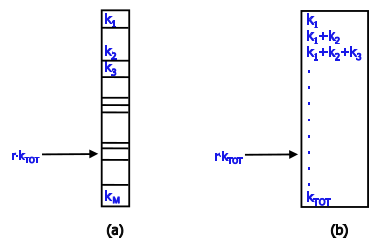
\includegraphics[width=0.7\textwidth]{numerics/images/nFoldWayRates}
  \end{center}
\end{figure}

I will defer to Voter (see in particular Sec. 5 of~\cite{voterKMC}) for the ``proof of correctness'' of the
method. The primary advantage of this method is that we are certain to advance time every step, so we are
not potentially
``wasting'' steps as
when we use even 
timestepping; this comes at the cost of having to compute which transitions are possible from the current
state. For our SPM, a given state has $\mathcal{O}(L)$ possible transitions, thus the time complexity
of a single timestep is $\mathcal{O}(L)$; note that our method with evenly-spaced timesteps has constant
time complexity, but the size of each timestep scales as $\mathcal{O}(L^{-1})$; thus we're not actually
losing as much as it appears by using variable timesteps. Furthermore, there is the possibility that the
process by which we calculate which transitions are possible could be performed in parallel, and so
the walltime cost of a single timestep in the n-fold way can end up comparatively cheap. The process of
choosing a successor state once the options are found involves performing the equivalent of a search, and
therefore takes $\mathcal{O}(\log{L})$ time and so should be insignificant.


\section{Implementation of Monte Carlo Methods}
\subsection{Our Implementation of a Metropolis-Hastings Algorithm with Evenly-Space Timesteps}
We have written a Fortran code which implements the algorithm in Sec. \ref{sec:evenTimesteps}. This is
stored in \cite{hellier2019a} in \texttt{evenTimesteps/evenTimesteps.f}. This programme initialises the system to have a particle density
equal to the average of the two desired boundary densities, and then proceeds in a manner extremely
faithful to the simple accept/reject algorithm.


\subsection{\texttt{KMCLib}} \label{sec:kmcLib}
The vast majority of our Monte-Carlo calculations have been performed using the n-fold way, described in
Sec. \ref{sec:nFoldWay}. This is implemented for continuous-time Markov processes on crystalline lattices
(of which the SPM is an example) in a software package called \texttt{KMCLib}, documented 
at~\cite{leetmaa2014KMCLib} developed by Dr Mikael Leetmaa.

\texttt{KMCLib} is a Python-wrapped C++ package. This means that the frontend, where one specifies the
system to be simulated, the data to be recorded, and how the simulation is run, is written in a Python
script; then, when this script is run, it executes C++ code in order to represent the system and
actually carry out the desired operations. Furthermore, \texttt{KMCLib} can perform calculations in
parallel if so desired. Whilst there exist examples~\cite{hoffmann2014kmos, spparks} of kinetic
Monte-Carlo codes other than \texttt{KMCLib}, we chose to use that one due to our familiarity with all
of the languages involved, and preference for a Python frontend.

Of course, setting up different calculations which vary different parameters or measure different things
require different scripts. Going through every script we wrote individually would not be particularly instructive;
therefore we have instead chosen to focus
upon a single set of codes designed to perform a particular calculation, which we have annotated and 
included in~\cite{hellier2019a} in \texttt{kmc/1d/currentCalc}; the intention is that a reader wishing to reproduce any of our results could do
so by performing a few simple modifications to the code listed there. A more comprehensive codebase is
stored at~\cite{hellier2019b}, but this is sparsely annotated working code, and so might not be as helpful.

A code which provides Python input for \texttt{KMCLib} is contained within 
\texttt{concFlow.py}. This script takes in several command line inputs. These provide the parameters for
a simulation of the SPM, with the desired value of $\lambda$, system size and boundary conditions. It 
then sets up the representation of the system configuration and the means to enumerate possible
transitions and their associated rates, as is necessary to implement the n-fold way.
The initial configuration is generated by randomly inserting particles into the system until its density
is equal to $\frac{1}{2}\left(\rho_0 + \rho_L \right)$; we then perform $N_{\mathrm{eq}}$ KMC steps in order to 
equilibrate the system (in case the initial configuration we chose was highly deviant from the norm
for the prescribed parameters). The actual measurements are performed by time-averaging values for system
quantities (e.g. the number of particles entering the system at one end) over $N_{\mathrm{meas}}$ steps,
relaxing the system (in other words, performing steps but taking no measurements) for $N_{\mathrm{req}}$ steps,
and then repeating this process $N_{\mathrm{pass}}$ times. This way, we can generate $N_{\mathrm{pass}}$ time-separated 
observations of, say, the total current through the system, and because we are relaxing the system 
between measurement runs we should not have to worry too much about the results being unduly correlated
with each other, (assuming we set $N_{\mathrm{req}}$ high enough).
Thus, we supply \texttt{concFlow.py} with the following parameters as 
command line inputs:
\begin{enumerate}
 \item The particle reservoir concentration at one end of the domain, $\rho_0$.
 \item The particle reservoir concentration at the other end of the domain, $\rho_L$.
 \item The value of $\lambda$ to use in the simulation.
 \item The system size, $L$.
 \item The interval between measurements performed by the analysis
 routines, $N_{\mathrm{anal}}$. This should be set to $1$ in order to measure the current.
 \item The number of equilibration steps, $N_{\mathrm{eq}}$.
 \item The number of analysis steps per pass, $N_{\mathrm{meas}}$.
 \item The number of reequilibration steps per pass, $N_{\mathrm{req}}$.
 \item The total number of passes, $N_{\mathrm{pass}}$, which give separate
 sets of observations, performed during this calculation.
 \item A timescale, $\delta t$, which indicates how often to evaluate,
 and to what accuracy to record, times, when measuring the number of 
 particles in the system. We recommend that this be small compared to the expected KMC timestep size.
\end{enumerate}

In terms of the output of the code, it produces a short file summarising the input parameters,
some trajectory dump information (usually redirected to \texttt{/dev/null} in order to save hard
memory, which is often in short supply), as well as data taken by measurement routines. We nominate,
from a suite of possible routines, which measurements we would like it to take during analysis phases.
Note that in our calculations, we do not use any quantity's value during particular KMC steps;
rather, we always average our quantities over some amount of time. This is partly because some of the
quantities we are interested in do not really have any value during a single timestep (e.g. the flux of
particles through one of the boundaries), and also because the amount of time spent in particular
configurations could potentially vary wildly between configurations. The amount of time spent in a
particular configuration in the n-fold way is drawn from an exponential distribution with decay rate
$k_{\mathrm{tot}}$, as we saw in Sec. \ref{sec:nFoldWay}; thus, one could easily imagine a
situation in which the transition time varies wildly. For example, say we have a system with very low 
$\lambda$. If this system was quite full, there would be few transitions possible, and those possible
transitions would likely occur with low rates, therefore the KMC timesteps would tend to be very long.
However, later during the same simulation we could find ourselves in a situation where the system is
less full, and so more transitions can occur, and generally with much higher rates, leading to much
shorter timesteps. Thus, we shouldn't really treat particular quantities derived from these 
configurations with an equal footing, as the amounts of time the system spends in each are so very 
different.

The precise nature of our time-averaging depends a little on the measurement in question. The types
of measurements we usually perform are the following, where $T$ is the total time elapsed during
our $N_\mathrm{anal}$ step measurement run:
\begin{itemize}
 \item \textbf{Current} We count the total number of particles which enter or leave a given boundary
 over the course of the measurement run. Let the number of particles entering and 
 exiting at the $0$ boundary be $u_0$ and $w_0$ respectively, and likewise for the $L$ boundary with
 $u_L$ and $w_L$. Then
 \begin{equation}
  J = \frac{u_0+w_L-u_L-w_0}{2T}
 \end{equation}
should be a good estimate of the total current through the system during that time period.
\item \textbf{Block Size Distribution} In one dimension, we can look at a configuration and count how
many contiguous runs (``blocks'') of particles there are of different sizes (e.g. size 1 means a single
particle sandwiched between adjacent vacancies). We can find the distribution of block sizes, weight it
by the length of the associated KMC timestep, and then add this to a running total. If we do this over
our $N_\mathrm{meas}$ analysis steps and then normalise, we can build a histogram of the block sizes
during that time period.
\item \textbf{Particle Density} Similarly, we can count the total number of particles in the system,
weight it by the length of the KMC timestep, and then use this to build another histogram of the
system particle density. By keeping track of particles entering and leaving the system, it would be
possible to code this very efficiently to take $\mathcal{O}(1)$ time; however, as our routine to detect
block sizes scans through the system and counts as it goes along, we have just opted for a simple
$\mathcal{O}(L)$ scan of the whole system for our density measurement as well.
\end{itemize}
Using these analysis routines, we can generate time-averaged values for particle density histograms,
the block size distribution and the current. By calculating $N_\mathrm{pass}$ separate instances of 
these observables, we get $N_\mathrm{pass}$ samples from the relevant distributions, and from there
we can probe the statistics of these variables.


\subsection{Managing \texttt{KMCLib} Calculations in Parallel} 
Of course, it is one thing to have a code which can run on a laptop to produce the output of a 
particular simulation over the course of a day. It is quite another undertaking to run thousands of
separate calculations in order to map out parameter spaces and compute derived quantities such as the
diffusion coefficient. 

We have been running our calculations on Edinburgh University's \texttt{Eddie3} computing cluster.
This machine does not boast the high level of processor interconnection density of \texttt{ARCHER}
or the extremely high working memory of \texttt{DiRAC}; however, for the purposes of our calculations
it turns out that we need neither. The KMC algorithm only stores a single state of the system under
simulation at any given time, therefore its space complexity only scales as $\mathcal{O}(L)$.
Furthermore, whilst \texttt{KMCLib} can be run in parallel mode in order to take advantage of
a multithreaded environment, this isn't actually an advantage when we wish to run very large numbers
of separately-parametrised calculations, as the total amount of CPU time required remains the same,
whilst incurring additional overheads associated with parallelism.
Therefore, we have used a single-threaded environment for all of the calculations featured in this
thesis.

In order to set up a batch of calculations, we use the following procedure, implemented by the codes
stored in \texttt{kmc/1d/} within~\cite{hellier2019a}:
\begin{enumerate}
 \item Create a batch of input files, in the subdirectory \texttt{jobInputs/}. In our setup, we
 require that files titled
 \texttt{testInput.}$i$ are generated, with $i \in [1, n]$ where $n$ is the total number of 
 calculations to be performed. These input files are typically generated by a code such as 
 \texttt{lambdaFlucCreator.py}; parameters which determine the overall structure
 of the system (e.g. $L$, the system size) will usually be held constant across calculations, whilst
 parameters such as the stickiness or the boundary densities will be varied between them. These input files contain a single line of code, which will be appended to \texttt{python } and called in the command line.
 \item In order to actually perform the calculations, we submit them as \texttt{gridengine} batch
 jobs. We  run the script \texttt{kmcSubmit.sh}, which submits the nominated tasks whose input
 files are in \texttt{jobInputs/}, using the scripts \texttt{kmcJobArray.sh} and 
 \texttt{initKmc.sh} for intermediate steps. \texttt{kmcSubmit} is also the place where we specify
 calculational parameters, such as maximum memory usage, maximum runtime, etc; these will be taken
 into consideration by \texttt{gridengine} when it comes to scheduling these calculations, so it
 is important that the maxima be relatively tight upper bounds, otherwise the calculation priority
 will be extremely low, assuming that the cluster in question is being simultaneously used for many other
 calculations.
 \item The jobs will then be executed, in their own time. The results will be placed in the location
 nominated by the input files.
 \item Once the run is complete, and the data has been saved, we are then ready to process it into a
 more useful format, in our case a data file which can be interpreted by Mathematica, the programme
 we used for most of our analysis and graphing. This is done using a script such a 
 \texttt{lambdaPostProc.py}. Note that such
 a script needs to be able to handle the fact that data may not be produced for some of the 
 calculations (around 5\% in our experience). The most likely source of the
 problem seems to be an issue with type conversion between Python and C++, which only seems to 
 become a significant issue in larger calculations.
\end{enumerate}
Throughout our calculations, we have stored data in a human-readable format, instead of
in a more compressed binary format. This is because we believe that the benefit of having a 
human-readable format, and therefore a much greater ability to look through data and check the 
output, outweighs the associated memory cost (around a factor of $10$ or so), 
especially given that any memory reduction attained due to such a format change wouldn't alter
what was feasible in terms of what we can afford to store.


\section{1D Calculation Results} \label{sec:1dMonteCarlo}
Most of the calculations we have performed are for the $1$-dimensional version of the SPM. As we 
have already performed calculations relating to $1$D behaviour in Ch. \ref{sec:analChap}
and Ch. \ref{sec:transRateChapter}, we already have results which can be compared directly to our
Monte Carlo calculations; thus, we will be plotting them together wherever we feel it is
appropriate.

In terms of what to calculate, we can use our previous calculations to motivate our future ones.
Using Monte Carlo, we can calculate the quantities we already investigated, such as current and 
particle density. In addition, we can also look at the time-evolution of particular configurations,
to gain insight into the mechanisms by which particles are transmitted during flow. This is
something our MFT says essentially nothing about, and our TRM calculations are too small to see 
anything meaningful in this regard.

\subsection{Flow Patterns} \label{sec:flowPatternVis}

First, let's talk about these flow patterns. Of the two methods available, we have only implemented
the visualisation of flow using the KMC calculations. This is because the n-fold way produces
a more ``realistic'' trajectory for the SPM, in the sense that the trajectory is an exact 
reproduction of the behaviour of the continuous-time Markov system; our other method, the simpler
accept-reject algorithm, should reproduce correct behaviour when long-term time averages are taken,
but might behave badly over small times. For example, in this method, there is a \textbf{minimum} timescale
over which \textbf{any} particle can move, which is not the case for KMC, with its random timestepping.

Whilst this random timestepping makes for a more formally correct trajectory, it does make it a
little more difficult to produce visualisations of particle trajectories. Our method for overcoming
this is as follows:
\begin{enumerate}
 \item Calculate a trajectory, with whatever choice of system parameters we like. The most 
 condensed way to do this in terms of hard memory during calculation runs is to keep track of which
 slots' occupancies change state at each 
 timestep, and retaining the timestamp of each timestep.
 \item From this occupancy data, we can use linear interpolation in order to assign a continuous
 occupancy variable to all sites at all times. Between timesteps, all sites not directly involved
 with a transition would have an occupancy of $1$ or $0$, and those involved in the transition
 would smoothly switch from occupancies of $0$ to $1$ and vice-versa.
 \item We can now make a new, evenly-stepped grid of space and time.
 We can integrate the interpolated KMC data over the time spacings of the new grid in order to
 find average occupations over the specified timeframe. 
\end{enumerate}
Thus, we can produce a spacetime diagram which shows the motion of particle density through the 
system over time. Clearly this method depends upon supplying a timescale $\delta t$ over which we
perform our averaging; a large $\delta t$ will ignore most of the specifics of the motion, whereas
a very small value will reveal a system in which only one particle is moving at any given time.

\subsubsection{Flow Visualization for Sticky Particles} \label{sec:1DStickyPlots}
We have performed calculations which illustrate the behaviour of an SPM system in $1$ dimension, displayed
in Fig. \ref{fig:1DStickyPlots}. These plots were generated by simulating SPM systems with $L=512$
and boundary conditions $(\rho_0 , \rho_L) = (0.75, 0.25)$, with $\lambda \in \{ 0.05, 0.15, 0.35 \}$.
We simulated over differing numbers of KMC steps, $N_\mathrm{steps}$, in the end performing
$N_\mathrm{steps} \in \{ 8192, 262144, 2097152, 8388608 \}$ steps respectively. Once the data was collected,
we could lookup the total elapsed time in each simulation, $T$, and then divide that time by $512$ in order
to obtain a discretization timescale $\delta t$, as required by our method for visualising flow patterns
described above in~\ref{sec:flowPatternVis}. In this way, we can visualise what the flow looks like over
different timescales for different values of $\lambda$. Note that the average size of a KMC step \textbf{does}
depend
implicitly on the value of $\lambda$; thus, the timescales portrayed in Fig. \ref{fig:1DStickyPlots}
are not consistent between the plots, as the timesteps are multiples of lengths 
$\sim \{ 6, 2, 1 \}\times 10^{-2} \mathrm{s}$ for $\lambda \in \{ 0.05, 0.15, 0.35 \} $ respectively. In
all of these plots, dark tones represent low time-averaged particle occupation, whilst light tones
represent high time-averaged particle occupation.
\begin{figure} \caption[The flow pattern of sticky particles in $1$D]{Spacetime plots of the particle flow
in 1 spatial dimension, as described in~\ref{sec:1DStickyPlots}. In each case, the $x$-axis represents \textbf{time}
and the $y$-axis \textbf{space}. The higher-density boundary is the one at the top of each image. Dark tones 
indicate low particle density, light tones high.} \renewcommand{\arraystretch}{-0.5}
\label{fig:1DStickyPlots}
\begin{center}
\begin{tabular}{c @{\hskip -0.5em} c| c @{\hskip -0.5em} c @{\hskip -0.5em} c} 
 & $\lambda$ & 0.05 & 0.15 & 0.35 \\
 $\frac{N_\mathrm{steps}}{8912}$ & & & &  \\ 
 \hline
 \rule{0pt}{0.1\normalbaselineskip} & & & & \\
 \raisebox{5em}{1}  &  & 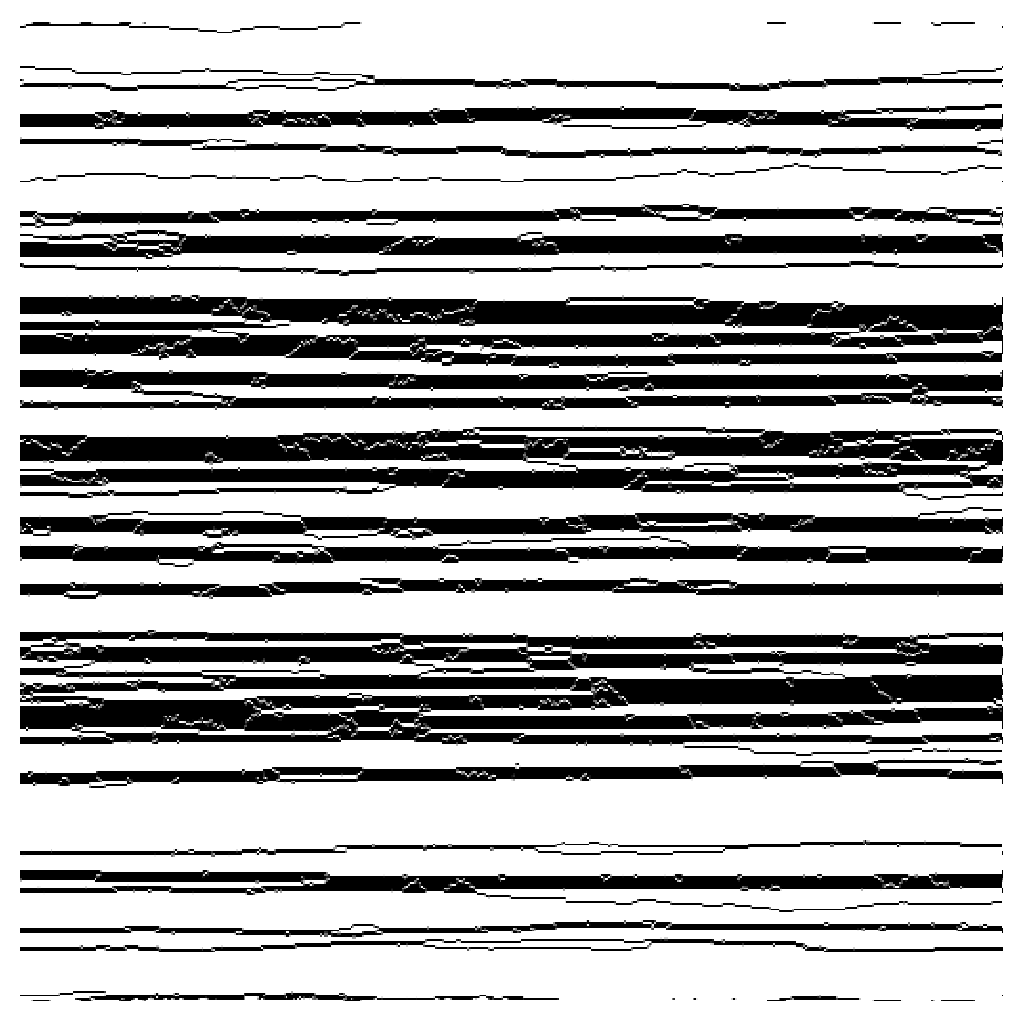
\includegraphics[width=0.31\linewidth]{numerics/images/stickyParticleFlows/flowImpL0p05T1p32.png}
 & 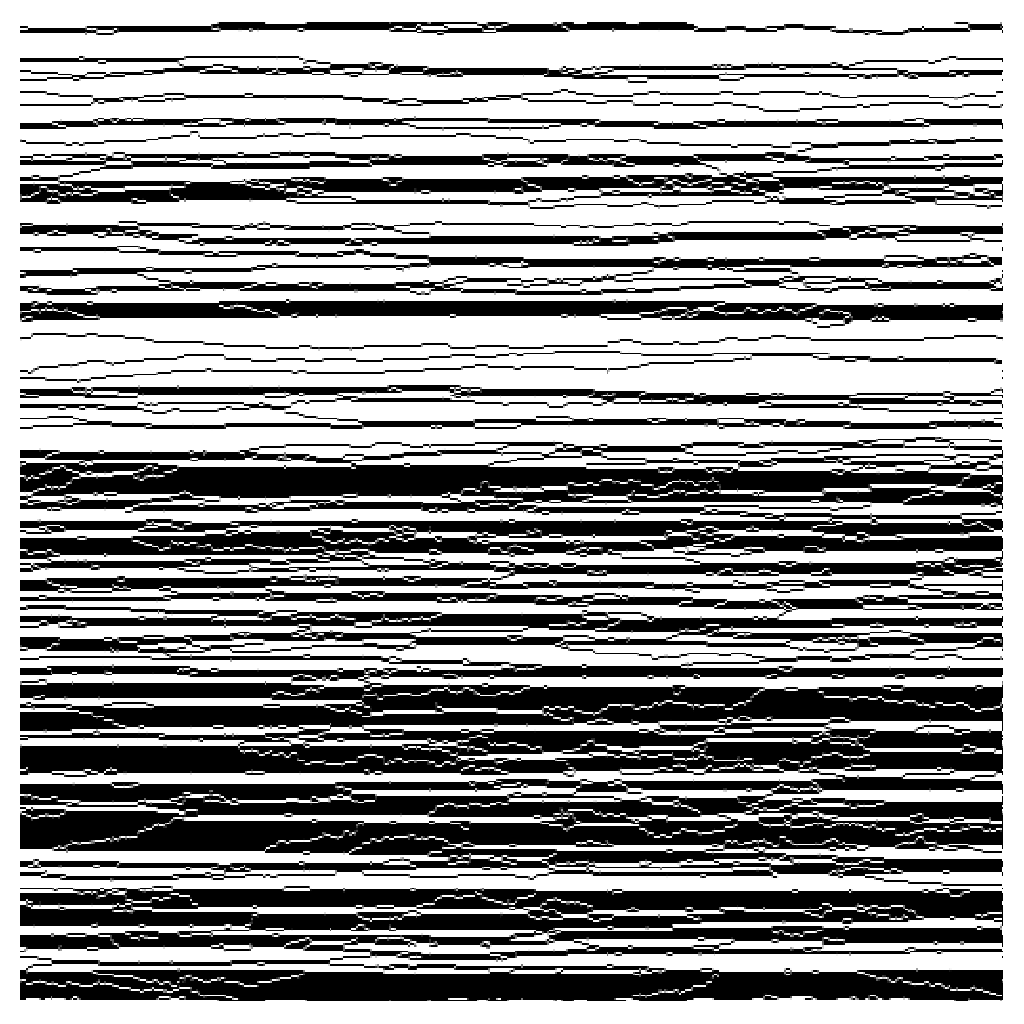
\includegraphics[width=0.31\linewidth]{numerics/images/stickyParticleFlows/flowImpL0p15T1p32.png} 
 & 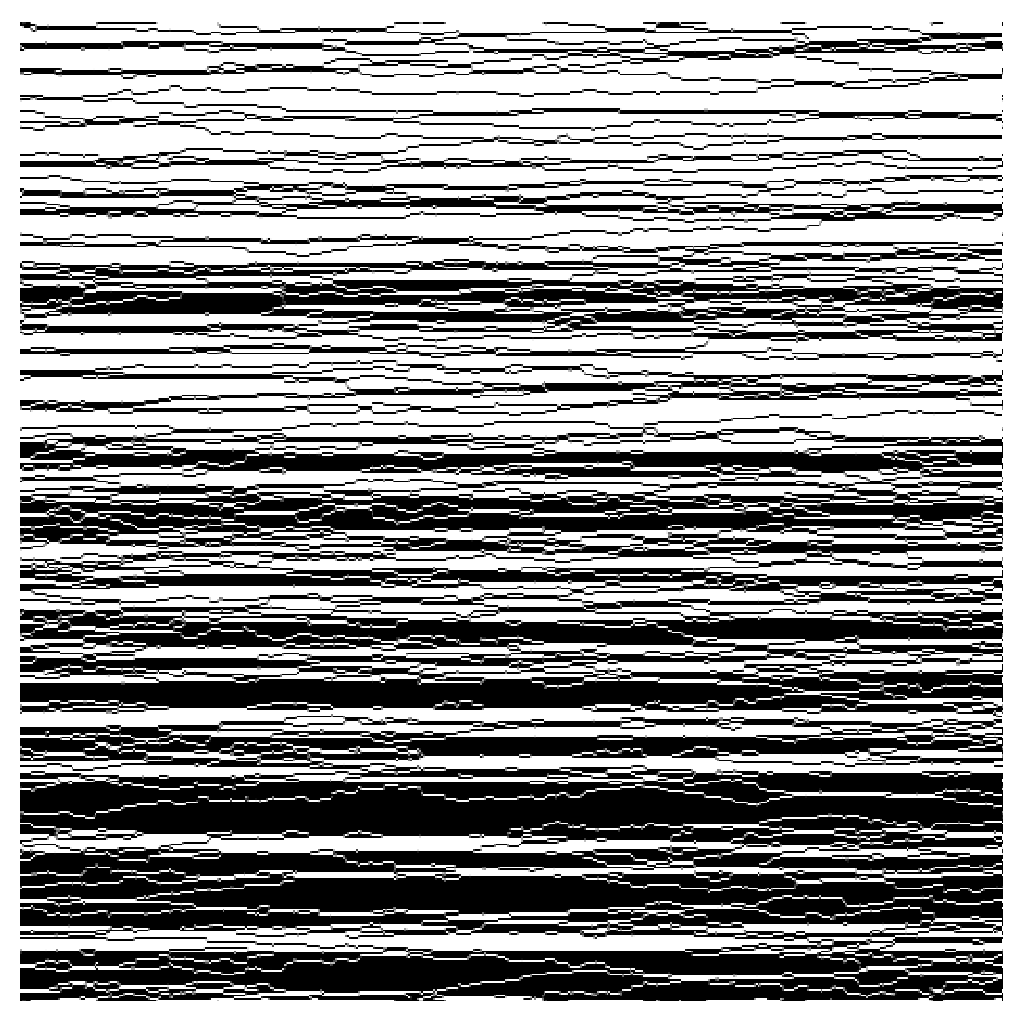
\includegraphics[width=0.31\linewidth]{numerics/images/stickyParticleFlows/flowImpL0p35T1p32.png} \\ 
\raisebox{5em}{32} & & 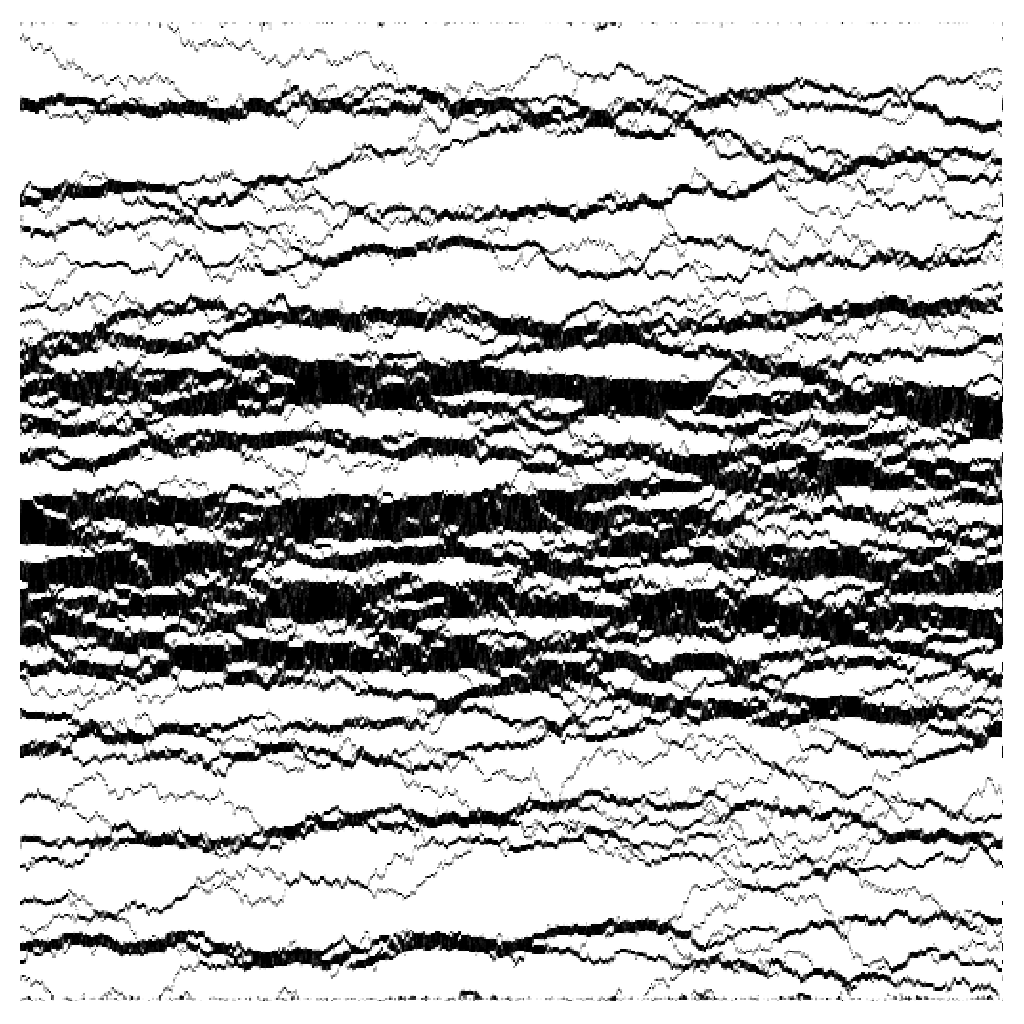
\includegraphics[width=0.31\linewidth]{numerics/images/stickyParticleFlows/flowImpL0p05T1p0.png} 
 & 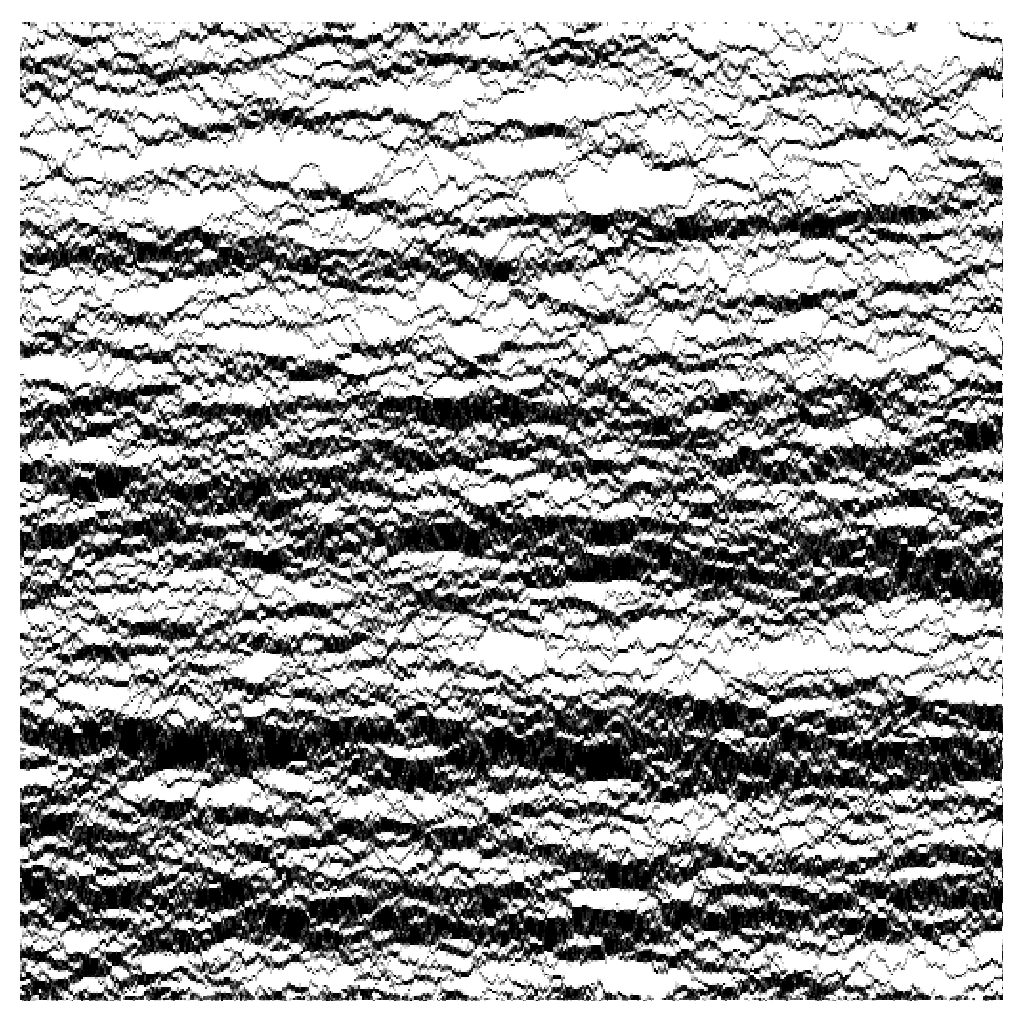
\includegraphics[width=0.31\linewidth]{numerics/images/stickyParticleFlows/flowImpL0p15T1p0.png} 
 & 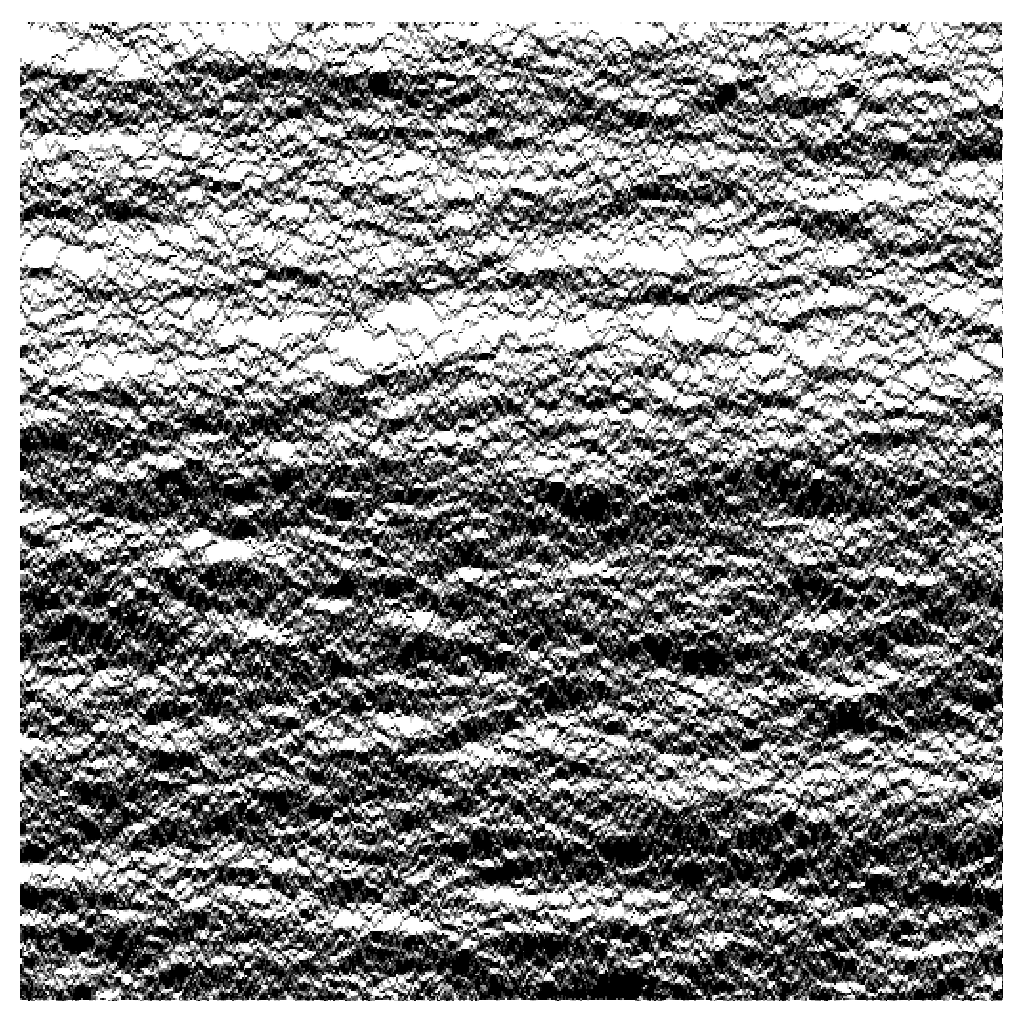
\includegraphics[width=0.31\linewidth]{numerics/images/stickyParticleFlows/flowImpL0p35T1p0.png} \\
\raisebox{5em}{256} & & 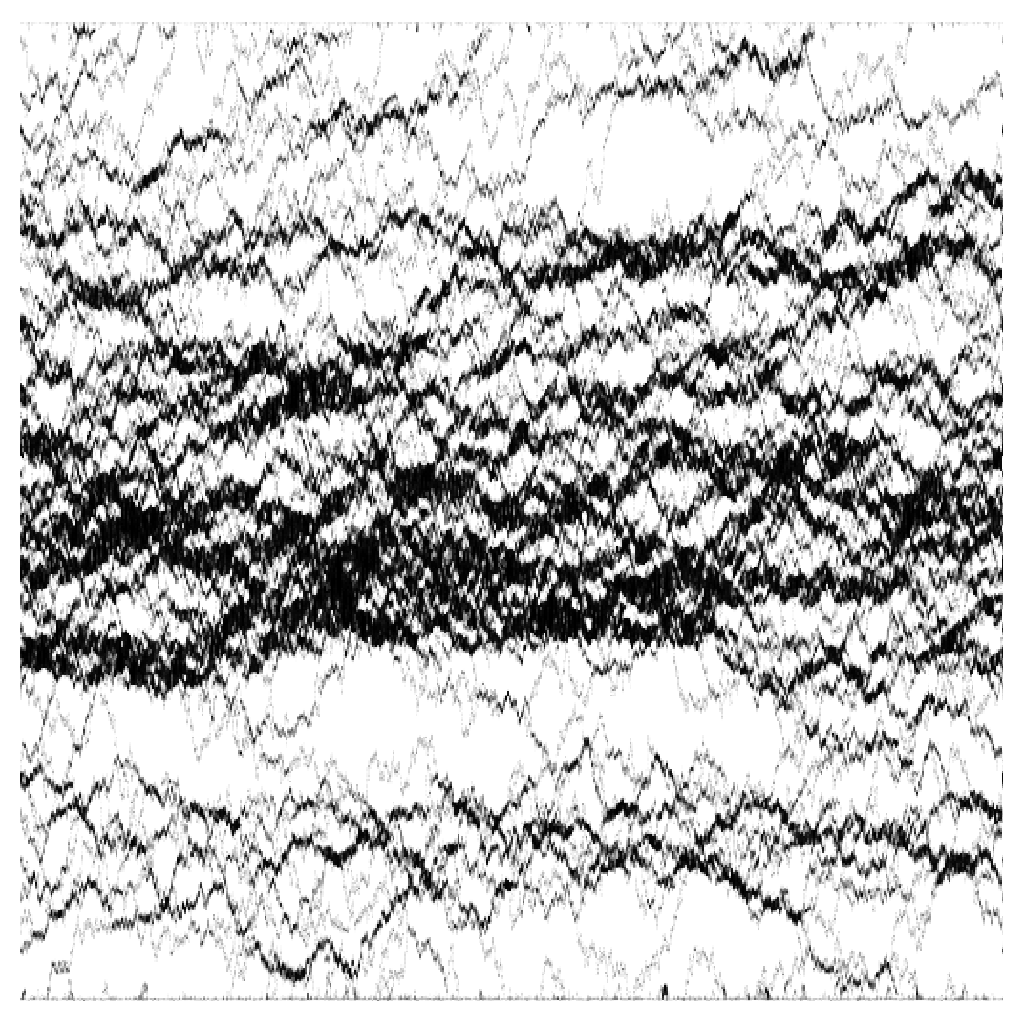
\includegraphics[width=0.31\linewidth]{numerics/images/stickyParticleFlows/flowImpL0p05T8p0.png} 
 & 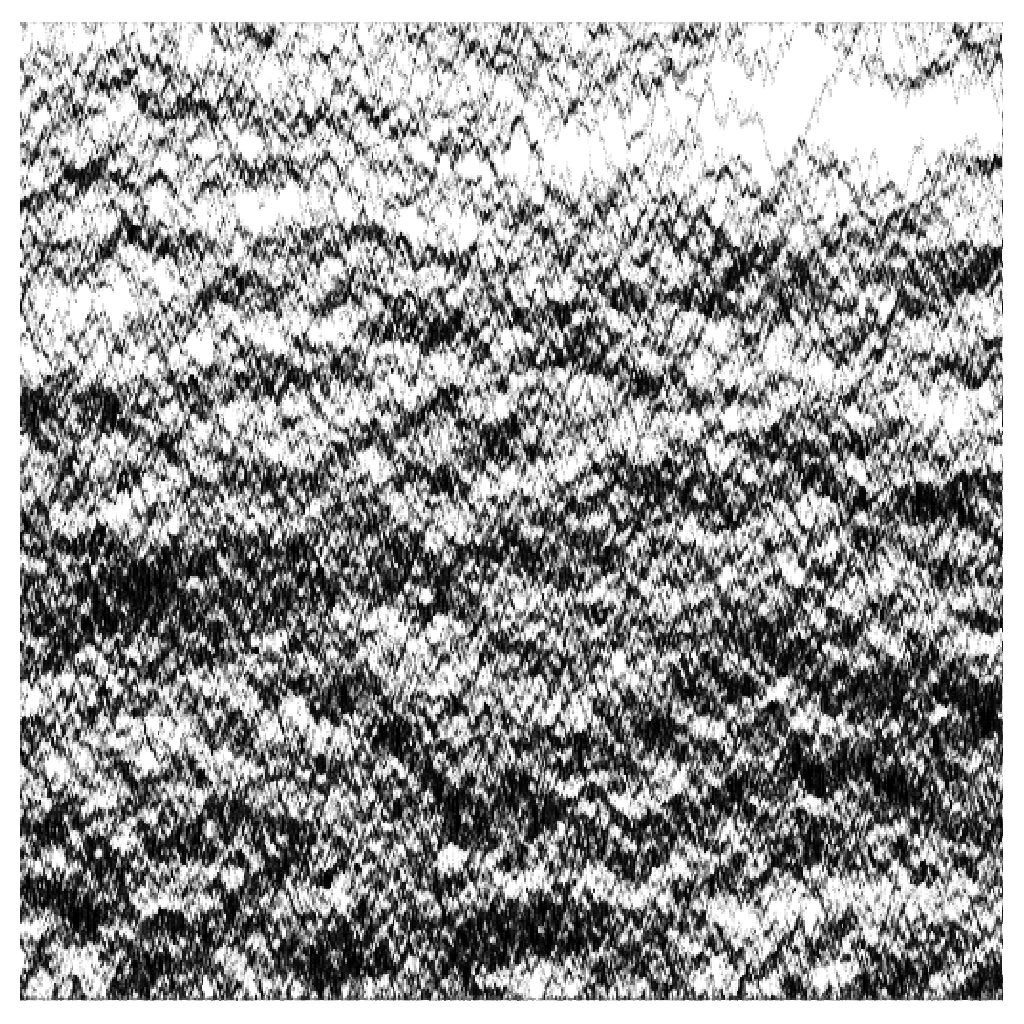
\includegraphics[width=0.31\linewidth]{numerics/images/stickyParticleFlows/flowImpL0p15T8p0.png} 
 & 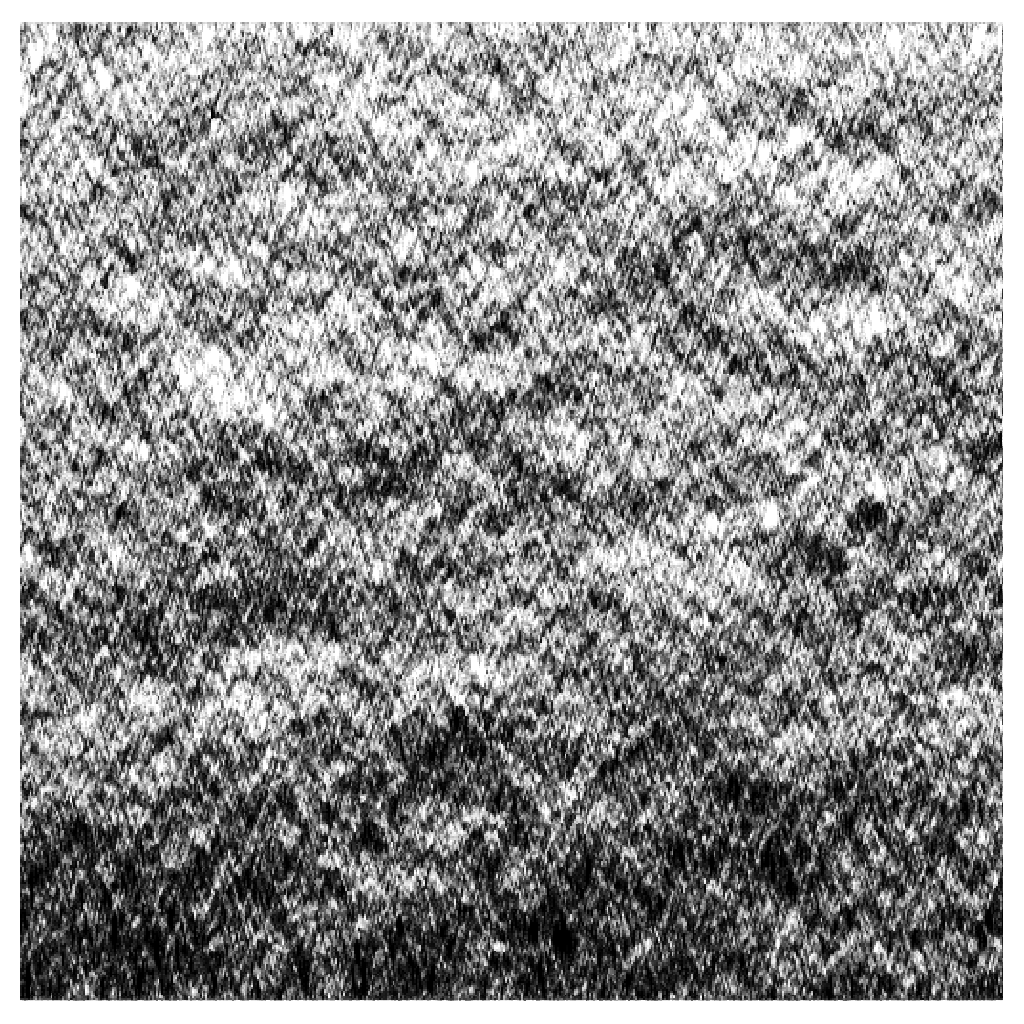
\includegraphics[width=0.31\linewidth]{numerics/images/stickyParticleFlows/flowImpL0p35T8p0.png} \\ 
\raisebox{5em}{1024} & & 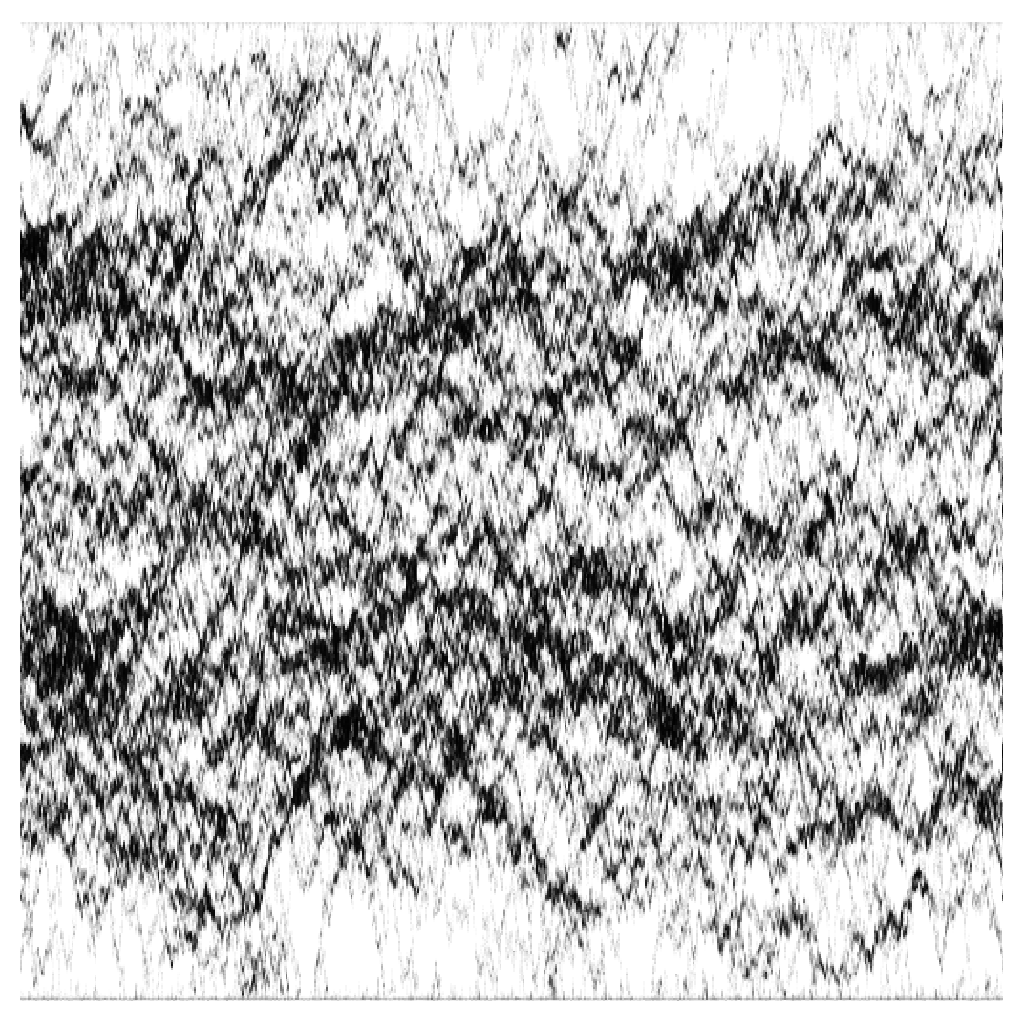
\includegraphics[width=0.31\linewidth]{numerics/images/stickyParticleFlows/flowImpL0p05T32p0.png} 
 & 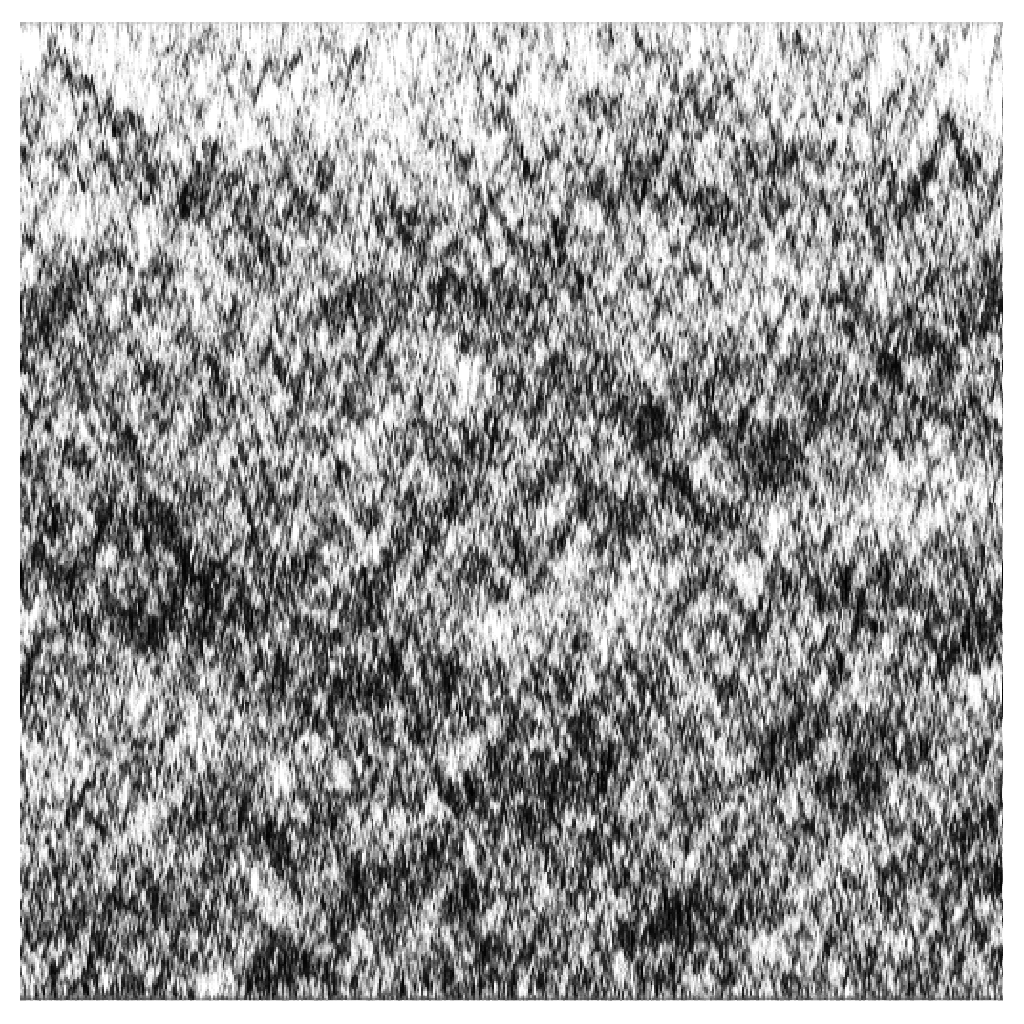
\includegraphics[width=0.31\linewidth]{numerics/images/stickyParticleFlows/flowImpL0p15T32p0.png}
 & 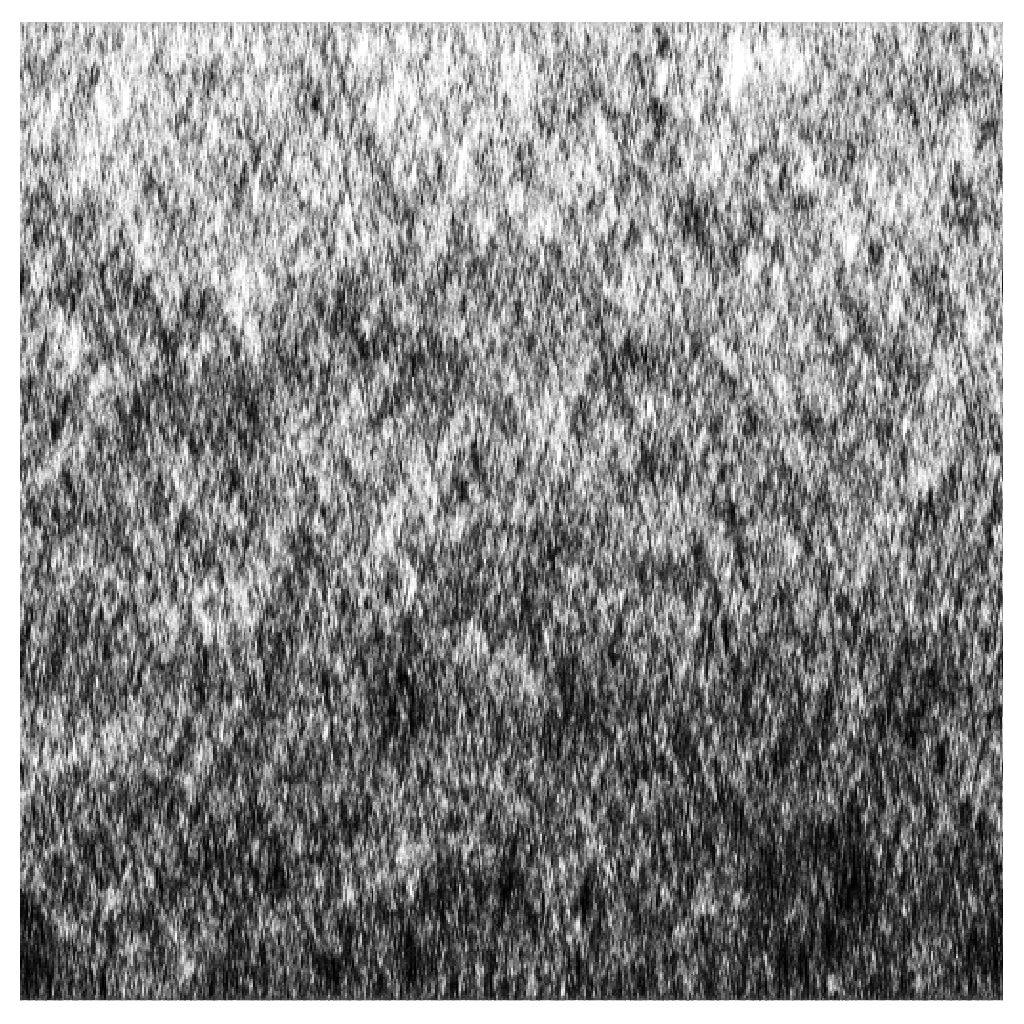
\includegraphics[width=0.31\linewidth]{numerics/images/stickyParticleFlows/flowImpL0p35T32p0.png} \\ 
\end{tabular}
\end{center}
 \end{figure}
 
Each of the systems here show the behaviour of particles with low-$\lambda$, so we are in the sticky regime;
however, all of our previous results indicate that there should be rather large differences in behaviour
as we switch from relatively weak stickiness (here embodied by $\lambda=0.35$) to strong stickiness
(portrayed by the $\lambda = 0.05$ situation). The images used to create Fig~\ref{fig:1DStickyPlots} are
relatively high-definition, which should enable readers using the digital copy to zoom in order to see the fine 
details. Our principle observations are as follows:
\begin{itemize}
 \item At the shortest timescale, one can quite clearly see the motions of individual particles. As one
 might expect, they are less likely to be seen unbound from neighbours in the lower-$\lambda$ systems than
 the higher-$\lambda$ ones. In the low-$\lambda$ regime, we are much more like to see big blocks of 
 particles, possibly containing a low concentration of mobile vacancies. Between these blocks we have a dilute
 ``gas'' of usually individual particles.
 \item Focussing now on the $32\times$ longer intermediate timeframe, we can see that in the extremely 
 low-$\lambda$
 situation we have blocks of particles separated by voids of vacancies. These voids contain a dilute gas
 of particles. Over these longer timescales, we see that the blocks of particles do in fact slowly migrate
 around the system, occasionally breaking apart or reforming during their travels. Also notice that the 
 voids are more likely to be found towards the centre of the system than adjacent to the boundaries.
 The chemical potential
 (Fig~\ref{fig:spmChemPot}) for small-$\lambda$ is minimised for high density, thus a boundary held at any
 density should be expected to in practise generate a high local density regardless of the density it is
 set to emulate; as we move away from the boundary its correlations with the interior weaken, so we think
 that the accumulation of particles on the boundary is an edge effect with a certain depth, and that the
 situation towards the centre of the system is more representative of the preferred bulk behaviour.
 \item Meanwhile for higher-$\lambda$, we see a ``tissue paper'' pattern over these intermediate
 timescales; the system is similar to a gas of randomly-walking particles, but there is a little bit more
 short-range correlation than that, hence the observed texture in the image.
 \item Now looking over longer timescales, we see that for the lowest-$\lambda$ it is in fact the case that 
 the voids towards the centre of the system do in fact appear and disappear over time. Given that we know 
 that there are still (small) flows occurring in this regime (see Sec. \ref{sec:lambdaScans}), it is
 likely that when these voids are created and destroyed, there are small overall biases in terms of
 which void boundaries more particles are extracted from or shed into. We suspect that
 this is the primary mechanism by which transport across the system is achieved in this regime. Meanwhile,
 the higher-$\lambda$ systems are becoming something closer to a continuous grey gradient from the top
 boundary to the bottom, suggesting that the overall transport is more diffusive in nature.
\end{itemize}



\subsubsection{Repulsive Particles}
Of course, we can do similar calculations with repulsive particles, for which $\lambda > 1$. Of the most
interest is the extreme case in which $\lambda >> 1$, when we should expect that particles have an almost 
explosive tendency to separate if brought together. We have performed such a calculation, with results
displayed in Fig~\ref{fig:1DRepulsePlots}, with a system
of length $L=1024$, $\lambda = 10^6$ and $(\rho_0 , \rho_L) = (0.99, 0.01)$, for which we performed $40960$
KMC steps. The time slices used in the plot are of size  $2 \times 10^{-7} \mathrm{s}$.
\begin{figure} \caption[The flow pattern of repulsive particles in $1$D.]{Spacetime plot for a system of 
repulsive particles. As before, time increases along the $x$-axis
and space along the $y$-axis. The top plot displays the time-dependent density using the normal shading scheme
(white is full, black is empty, grey indicates partial occupation). In the bottom plot, we invert the shading scheme
every other site; thus, regions populated with alternating particles and vacancies are now displayed as solid blocks,
with the moving boundaries between those blocks being domain walls.} 
\label{fig:1DRepulsePlots}
\begin{center}
\begin{tabular}{c} 
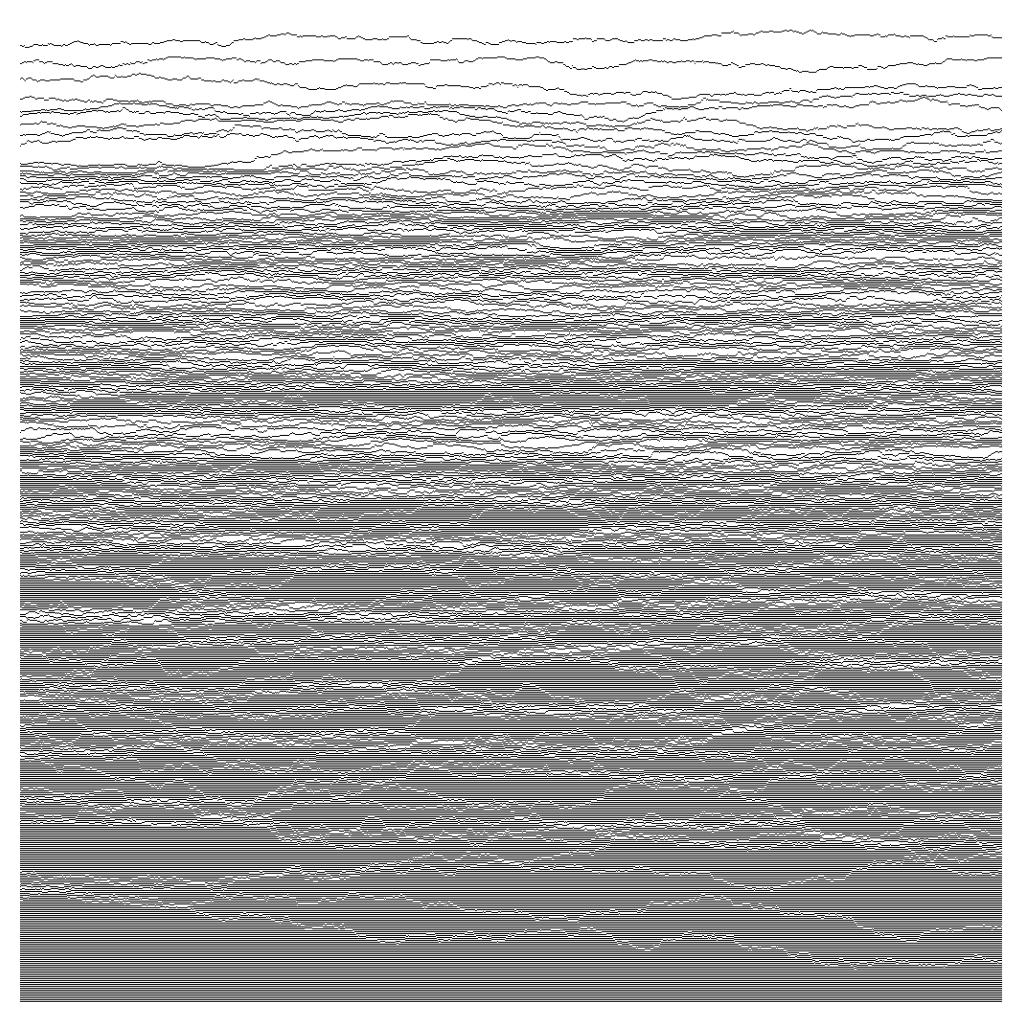
\includegraphics[width=0.65\linewidth]{numerics/images/stickyParticleFlows/aprilFlowStraight.png} \\
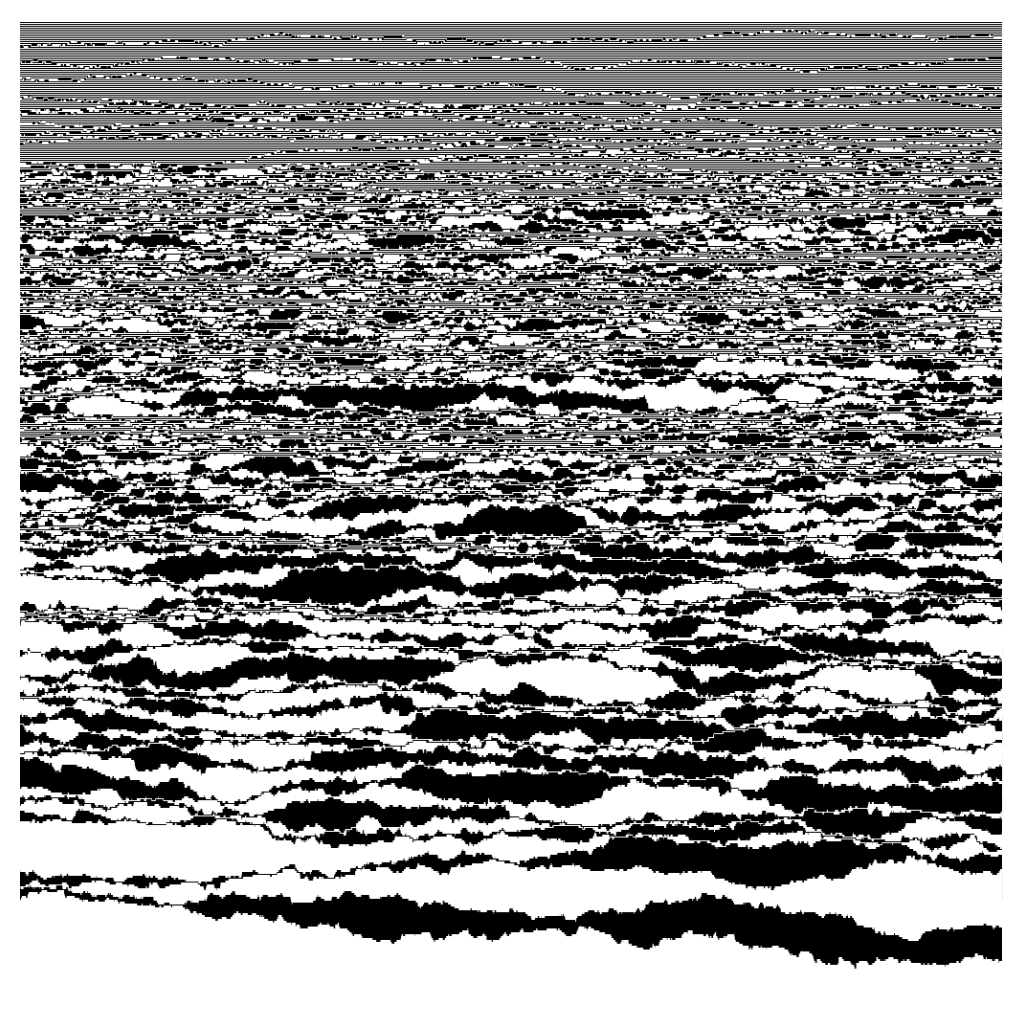
\includegraphics[width=0.65\linewidth]{numerics/images/stickyParticleFlows/aprilFlowDomains.png} \\
\end{tabular}
\end{center}
 \end{figure}
 
As before, time goes from left to right, space from top to bottom. 
The top plot displays the time-averaged density shaded the normal way (light being dense, dark being empty).
The bottom plot displays the same information, only this time we have applied the function $f(x) = 1-x$
to the density at every other site as we move along the spatial axis; thus we reveal that in this limit
our system is partitioned into domains, in the same way that an antiferromagnet might be. The boundaries
between these domains can move quite rapidly, and the motion of such a domain wall corresponds to the
transport of a particle; thus we think that it is this domain boundary motion which controls the rate
of transport in this regime.
 
 
\subsection{Scans Through $\lambda$ with Constant Boundary Densities} \label{sec:lambdaScans}
We can perform calculations in which we hold all things constant except $\lambda$, analogous to our 
existing calculations done using our TRM and MFT results. In these calculations, we computed the properties of systems with boundary densities $(\rho_0 , \rho_L )=(0.3, 0.1)$, $(0.75, 0.25)$ and 
$(0.9, 0.7)$, using both the evenly-timestepped Monte Carlo method and KMC. In this case, our KMC calculations used systems of size $L = 64$, whilst our other method used systems of size $L=100$.
To account for the different system sizes used, we have rescaled the current and its moments, whilst
leaving most other quantities such as particle density as they are. In the case of current, we have
multiplied by $L$ in order to achieve this normalisation; this is because a normal diffusive current is
driven by concentration gradient, therefore if we use the same concentration difference we should expect 
the resulting current to vary as $J \sim L^{-1}$. Note that for our KMC calculations we performed initial
equilibration runs of $4000000$ steps, followed by $1000$ of our alternating analysis/relaxation passes
of $16000$ steps each way; thus, this should provide us with decent quality data, at least until $\lambda$
becomes so small that particles can barely move through the system. Our evenly-timestepped calculations
were performed with $10000$ equilibration steps followed by a single measurement run of $100000000$ steps,
so we aren't calculating the other moments of the current using that method.

\subsubsection{Mean Current}
\begin{figure} \caption[The current flowing through systems as we vary $\lambda$ with constant boundaries,
$1$D]{The mean current observed to flow from a boundary with greater particle density to lesser particle 
density in $1$D. Here the boundary densities are held constant throughout, whilst $\lambda$ is varied.
The lower plot is the same data as the upper one, but with logarithmic axes instead of linear ones.
The dashed lines
correspond to the MFT predictions, the joined circles to TRM-computed results, the triangles to results
computed using evenly-timestepped Monte Carlo and the crosses to KMC calculations. Note that we do not have reliable
error estimates for the evenly-timestepped Monte Carlo calculations.} 
\label{fig:1DlambdaScans}
\begin{center}
\begin{tabular}{c} 
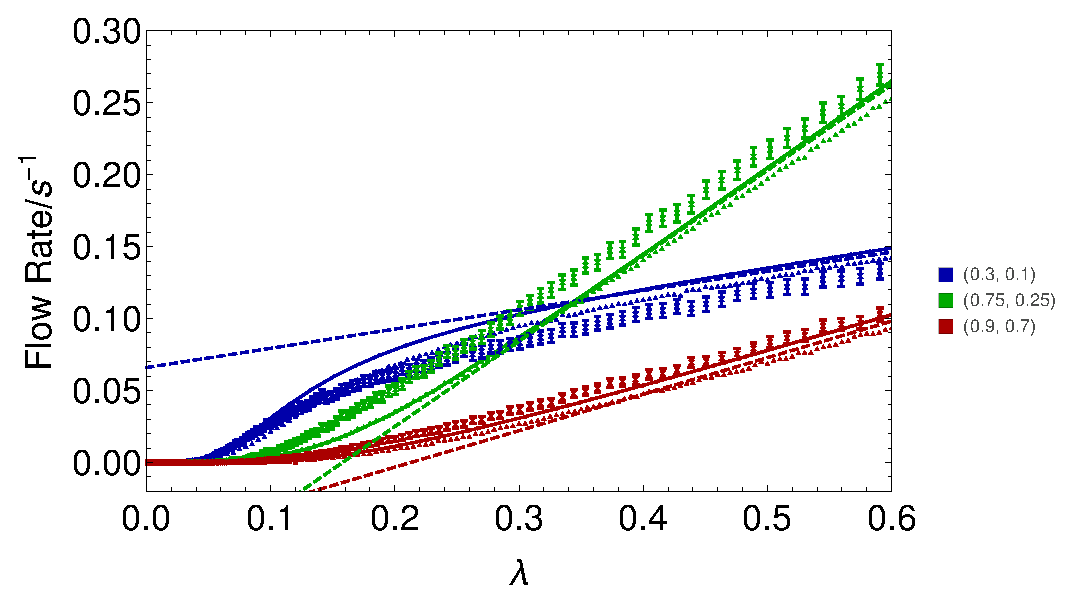
\includegraphics[width=1.1\linewidth]{numerics/images/lambdaScan/correctionsCombinedLinear} \\
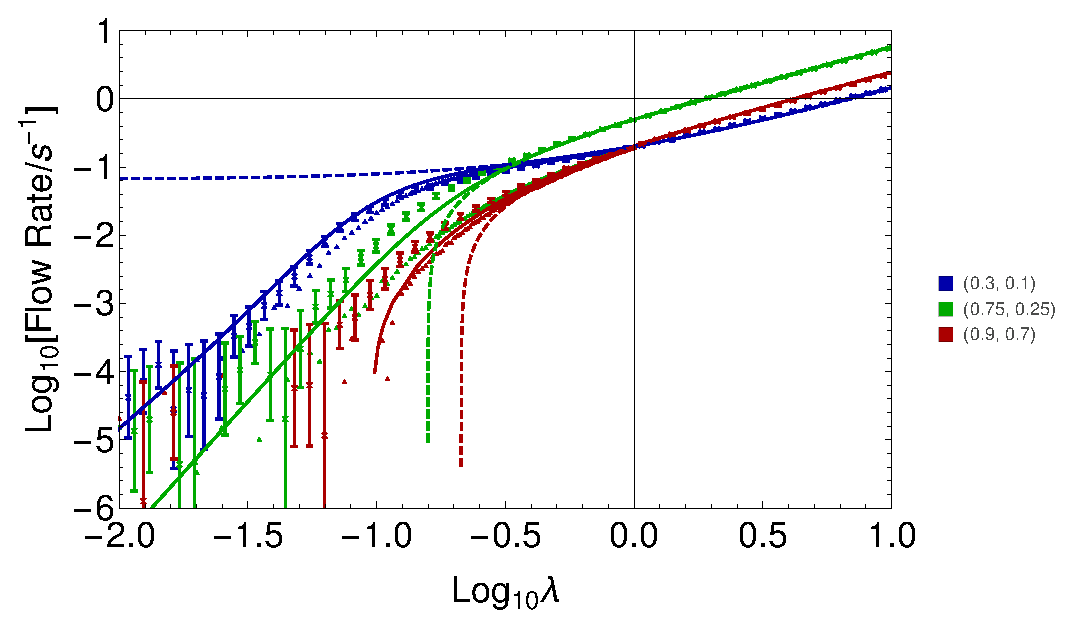
\includegraphics[width=1.1\linewidth]{numerics/images/lambdaScan/correctionsCombinedLogSmall} \\
\end{tabular}
\end{center}
\end{figure}

Fig. \ref{fig:1DlambdaScans} displays the variation of the current with $\lambda$. Here, the dashed lines
correspond to the MFT predictions, the joined circles to TRM-computed results, the triangles to results
computed using evenly-timestepped Monte Carlo and the crosses to KMC calculations.
Fig. \ref{fig:1DlambdaScansLogged} displays the same data, but over a wider range of $\lambda$ values.
We have already discussed the TRM results and their relation to the MFT results back in 
Sec. \ref{sec:TRMLambdaScan}. Our main observations about the current are as follows:
\begin{itemize}
 \item At large $\lambda$ the current seems to vary in proportion to $\lambda$, in agreement with our
 TRM and MFT results. The actual constants of proportionality don't quite match, which is a common issue
 in all of these results. We have seen in Sec. \ref{sec:flowPatternVis} that there is usually a boundary
 layer of excess particles or vacancies next to both boundaries, thus it is possible that this issue
 arises from this boundary layer causing the current to not scale with $L$ in quite the way we
 expect. However, this is something we can check by varying the system size and checking the current
 variation with $\lambda$, as we have done in Figs.\ref{fig:lambdaScanRepeats}.
 \item For $\lambda \in (0.01, 0.3)$, the current undergoes power law variation with $\lambda$, again in 
 agreement with our TRM calculations, with $J \propto \lambda^{3}$.
 \item For smaller values of $\lambda$, the observed mean current starts to become noisy, at least in the
 logarithmic plots, and essentially saturates to a low value. Our interpretation of this is that for these
 extreme low values of $\lambda$ the current signal becomes extremely weak, as it begins to depend on the
 motions of extremely small overall numbers of particles during the measurement period; thus, in that 
 regime the current is dominated by a form of shot noise, and so it becomes difficult to measure the current accurately in this regime.
\end{itemize}

\begin{figure} \caption[As Fig. \ref{fig:1DlambdaScans} but over a much wider range of $\lambda$-values.]{As the logarithmic plot in Fig. \ref{fig:1DlambdaScans} but over a  much wider range of $\lambda$-values.} 
\label{fig:1DlambdaScansLogged}
\begin{center}
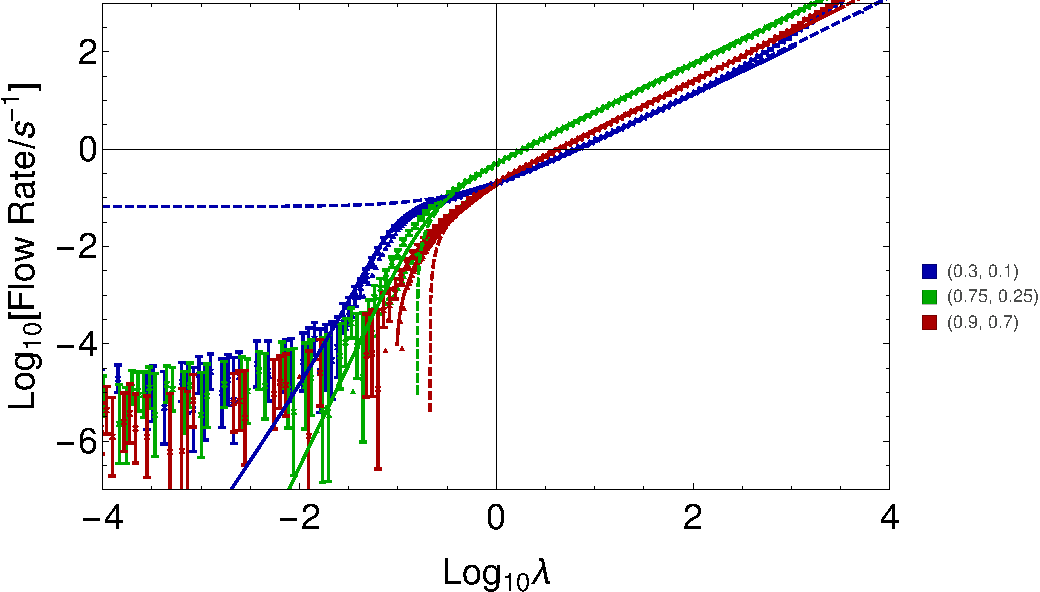
\includegraphics[width=0.9\textheight, angle=270]{numerics/images/lambdaScan/correctionsCombinedLogLarge}
\end{center}
\end{figure}

\begin{figure} \caption[Comparison of the variation of the mean current with $\lambda$ for different system sizes.]{As
Fig \ref{fig:1DlambdaScans}, but we are now comparing Monte Carlo results from systems of different size instead of 
the other calculation methods. Here, \textbf{circles}, \textbf{squares} and \textbf{triangles} represent systems of 
size $L=32$, $64$ and $128$ respectively. The currents computed have been normalised via multiplication by $L$.
Note that all error bars are present; when invisible, this suggests that they are smaller than symbol size. We believe
that the errors for the extreme low-$\lambda$ regime are underestimates, due to the systems not having had time to
fully equilibrate. MFT results are displayed for comparison as solid curves.} 
\label{fig:corrLambdaScans1d}
\begin{center}
\begin{tabular}{c} 
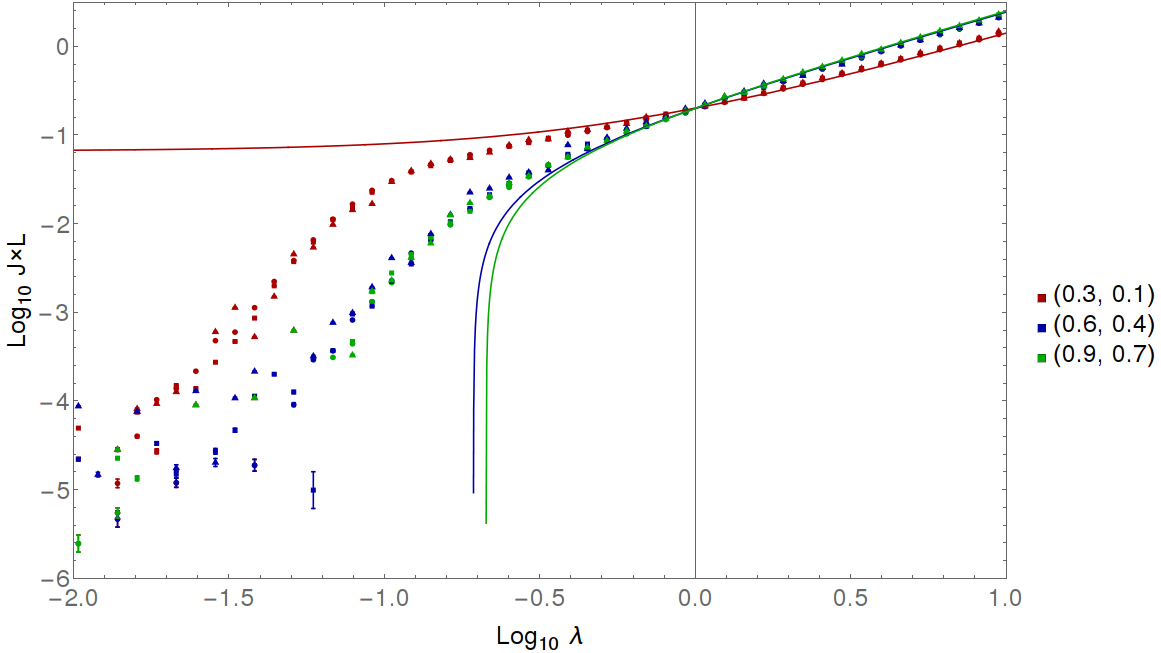
\includegraphics[width=1.1\linewidth]{numerics/images/lambdaScan/correctionsLambdaScan1dSmall} \\
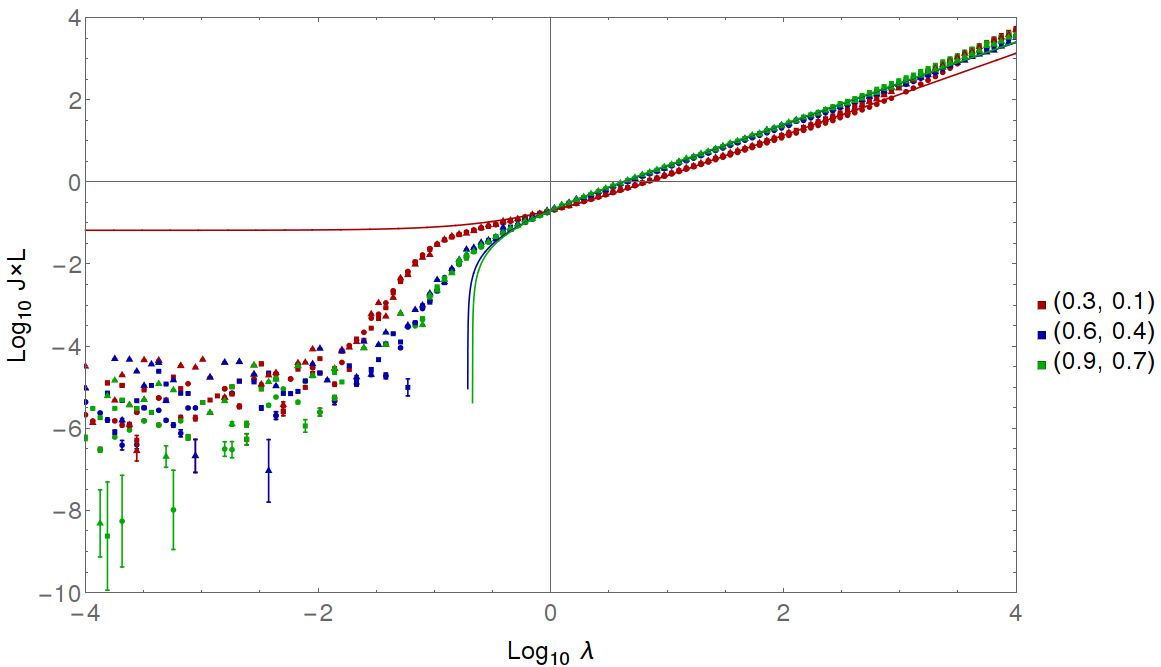
\includegraphics[width=1.1\linewidth]{numerics/images/lambdaScan/correctionsLambdaScan1dLarge} \\
\end{tabular}
\end{center}
\end{figure}

Thus, we still seem to see the same ``transition'' we saw when analysing TRM results. To ensure that this
behaviour in the current isn't just an artefact of system size, we can vary the system size whilst
measuring the current, as we have done in Figs. \ref{fig:corrLambdaScans1d} and \ref{fig:lambdaScanRepeats}.
\begin{figure} \caption[Calculations of the dependence of current upon $\lambda$, repeated with different system sizes.]{Calculations of the dependence of current upon $\lambda$, repeated using KMC with different system sizes as indicated. Here we have focussed on the boundary setup 
$(\rho_0, \rho_L) = (0.75, 0.25)$ and region $\lambda \in (0.04, 0.25)$, which constitutes the
bend in our supposed transition. Standard errors in the current were computed using observed current 
variances. The fact that the errors seem to increase with system size suggests that the larger systems are fluctuating
more due to poorer equilibration.} 
\label{fig:lambdaScanRepeats}
\begin{center}
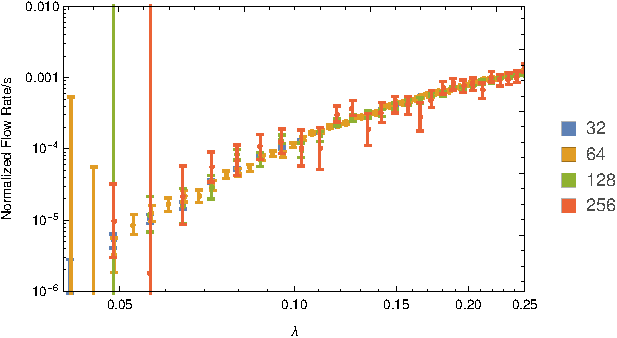
\includegraphics[width=0.8\textheight, angle=270]{numerics/images/lambdaScan/lambdaScanRepeatFlows}
\end{center}
\end{figure}

Here we see that our method for normalising currents for different system sizes actually seems
to work quite well, at least over the system sizes we are looking at. It also indicates that our choice of
$L=64$ behaves well until $\lambda < 0.05$, at which point the fluctuations start to become very large 
compared to the observed mean current.

An important thing to note here is that the critical $\lambda$ at which the ``transition'' occurs does
\textbf{not} seem to be sensitive to the system size. Similarly, the $\lambda$ at which the results ``plateau''
and reduction in $\lambda$ no longer meaningfully reduces the current also depends very weakly upon system size,
if at all. This plateau is presumably due to the flow becoming so slow that the number of particles moving in
and out of the system over a given timeframe is becoming so small that it becomes very susceptible to noise,
and so when we plot logarithmically we see the plateau with many results scattered under it.

\subsubsection{Current Higher Moments}
Using our KMC calculations, we can also compute the higher moments of the current. As we do not have any 
particular theory which predicts these higher moments, we do not have very much to say about these
results, other than simply stating what we see. It is worth noting that we don't detect divergences
in these moments around the bend of our ``transition'', therefore it does not seem to be a transition
in the traditional phase transition sense, as there we would expect to see discontinuities in observables,
and here current is the kind of observable we should expect to manifest that kind of behaviour.
These moments, up to and including the current kurtosis, are displayed in 
Fig. \ref{fig:lambdaScanHigherMoments}. Note that no units for skewness and kurtosis are listed
as they have already been normalised using the scale set by the variance.
\afterpage{
\begin{figure} \caption[Higher moments of the current, in 1$D$]{The higher moments of the current, 
measured using KMC in the same setup as used in Fig. \ref{fig:1DlambdaScans}. Note that we do not have reliable error estimates
for these quantities, as their computation would require good knowledge of these same higher moments; given the 
already dubious quality of the skewness and kurtosis readings (which one can assess visually from the spreading of  
nearby points on the graph), we can't make a proper assessment of the error in the variance.} 
\label{fig:lambdaScanHigherMoments}
\begin{center}
\begin{tabular}{c} 
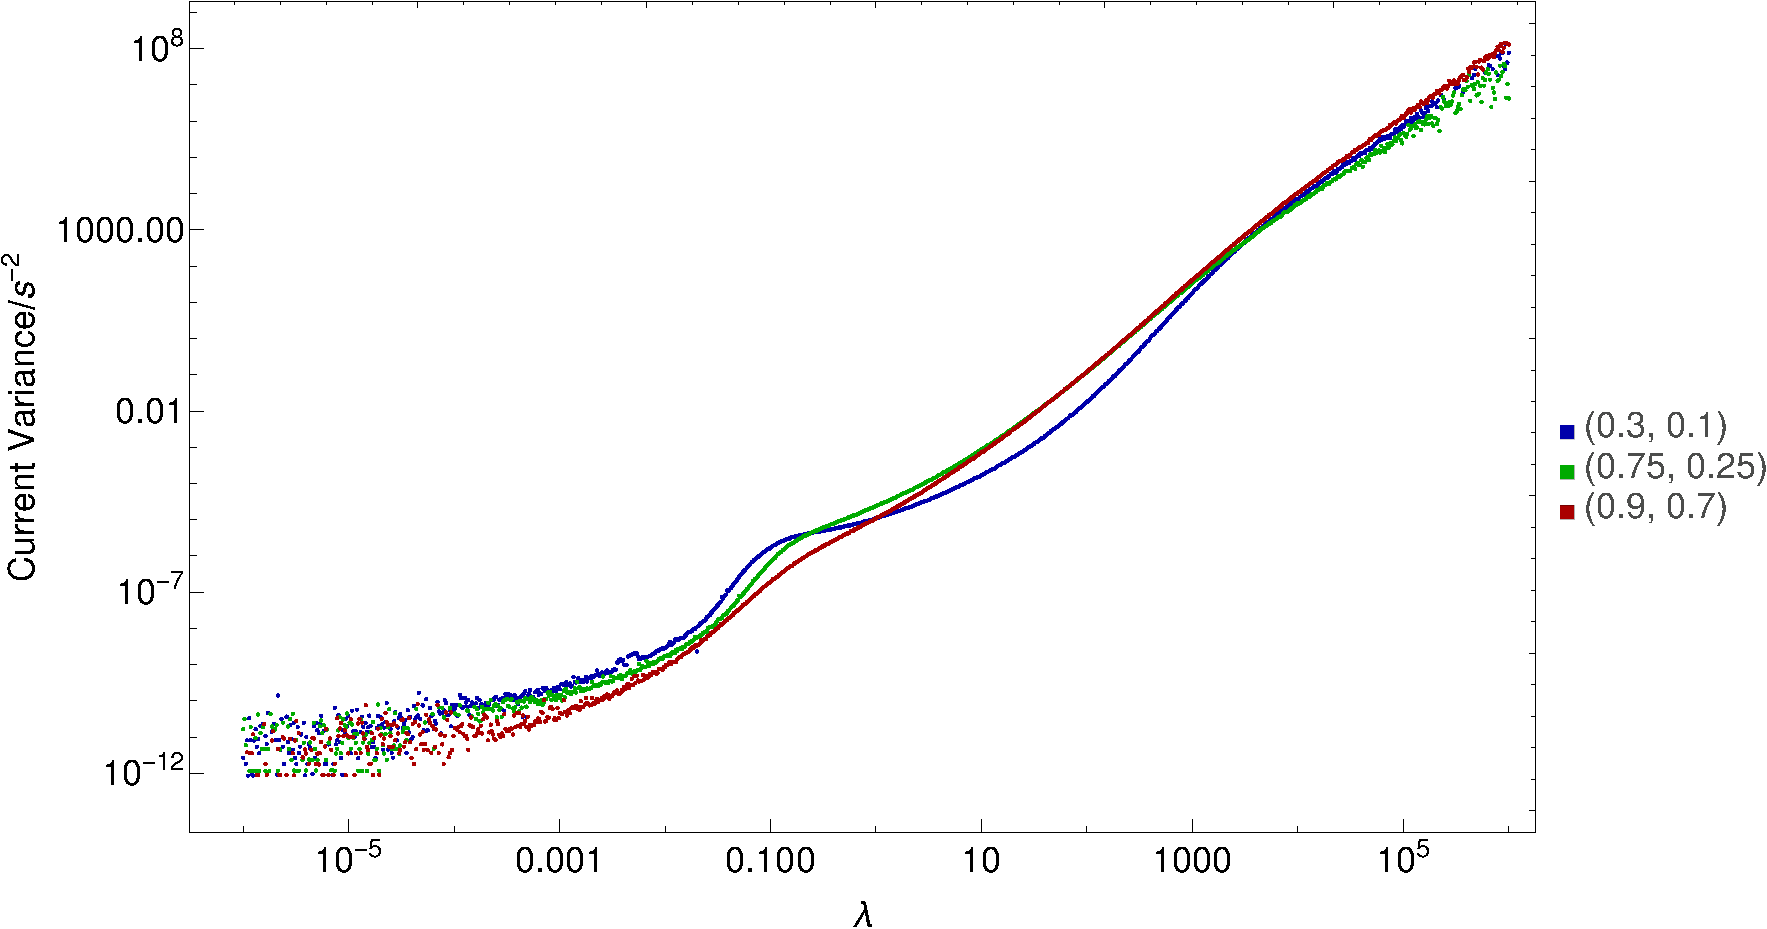
\includegraphics[width=0.8\linewidth]{numerics/images/lambdaScan/lambdaScanVar} \\
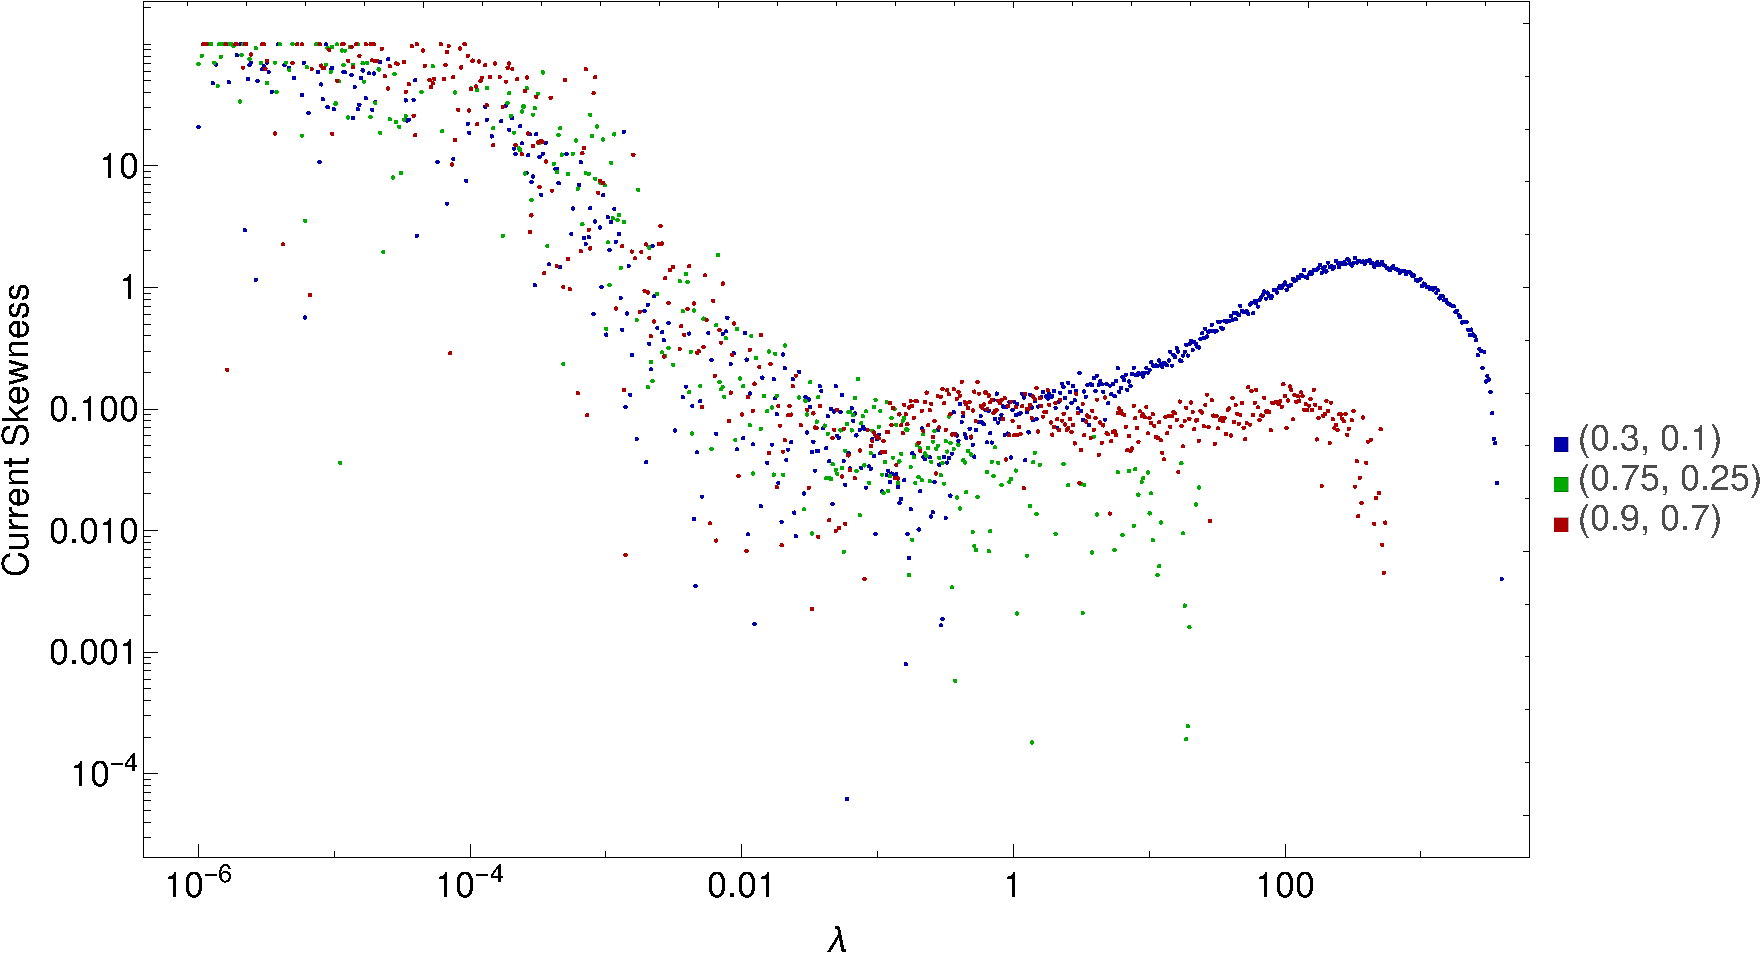
\includegraphics[width=0.8\linewidth]{numerics/images/lambdaScan/lambdaScanSkew} \\
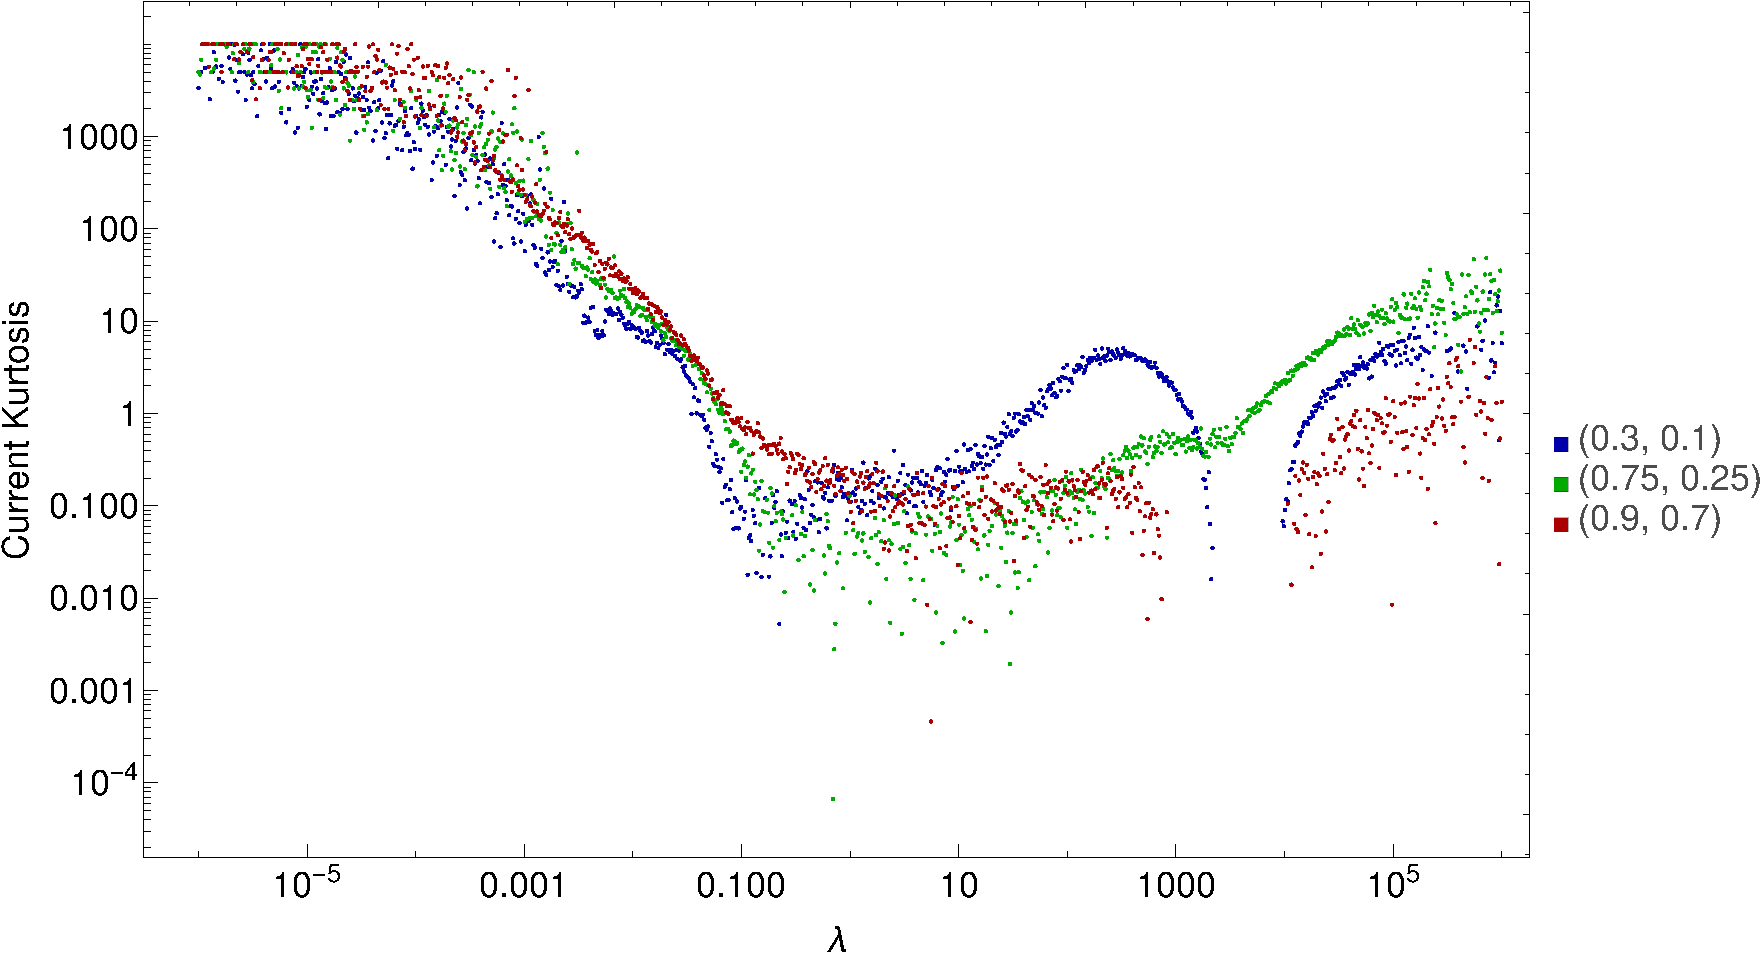
\includegraphics[width=0.8\linewidth]{numerics/images/lambdaScan/lambdaScanKurt} \\
\end{tabular}
\end{center}
\end{figure}
\clearpage
}

There's a little bit of a bend in the variance as we go through the transition, but nothing major.
Skewness is typically positive but fluctuates a lot, and goes negative past certain thresholds at
large $\lambda$. Kurtosis is bounded and possibly negative for $\lambda$ above the transition threshold,
then starts growing large and positive as we go through the suspected transition.
Thus, we have several different pieces of weak evidence of something happening in the transition region,
but nothing clear and conclusive like a spike or discontinuity.


\subsubsection{Overall Density}
\label{sec:ovDens}
In addition to measuring current and its moments, we can measure the mean overall density of particles in
the system. We did this using the same system parameters as in Fig. \ref{fig:1DlambdaScans}; the 
variation in this mean density with $\lambda$ for different boundary conditions is displayed in 
Fig. \ref{fig:lambdaScanDensityMean}.
\afterpage{
\begin{figure} \caption[The variation of the overall mean density of the SPM system with $\lambda$ for different boundary conditions, in $1$D.]{The variation of the overall mean density of the SPM system with $\lambda$ for different boundary conditions, in $1$D. 
Setup is the same as in Fig. \ref{fig:1DlambdaScans}.} 
\label{fig:lambdaScanDensityMean}
\begin{center}
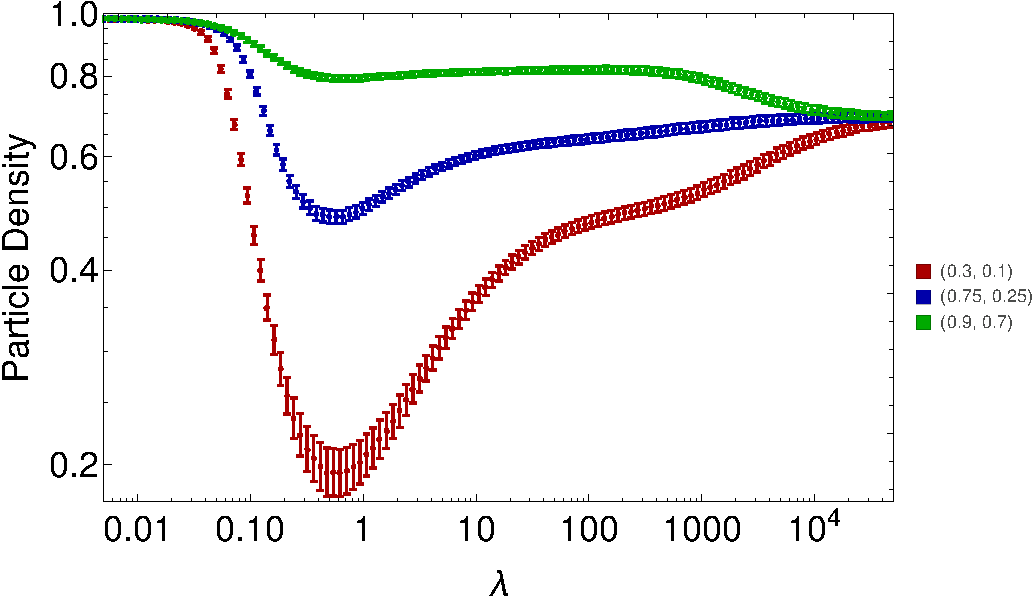
\includegraphics[width=0.95\textheight, angle=270]{numerics/images/lambdaScan/correctionDecWideDensProfiles}
\end{center}
\end{figure}
\clearpage
}

The most striking feature here is how the densities converge for extreme values of $\lambda$
regardless of the actual boundary conditions used, converging to $1$ for extremely small $\lambda$ and to
around $\frac{2}{3}$ for extremely large $\lambda$. The behaviour seen here is in accordance with our 
existing computations as seen in \ref{sec:TRMDensityCurrent}, and our theory about this is as expressed 
there: in short, that at small $\lambda$, high density is favoured for ``energetic'' reasons (the
attempted minimisation of equilibrium  free energy), whilst at very large $\lambda$  our system self-
organises to have a density of $\sim \frac{2}{3}$ in order to enable maximal flow to occur due to a
stability argument.

We can also measure the variance of the densities we observed, and use this to gauge the size of the
density fluctuation, $\Var(\rho) = \Var(N)/L$, where $N$ is the number of particles in the system.
In the results displayed in Fig. \ref{fig:lambdaScanDensityFluc}, we have
computed the density fluctuation in our $1$D SPM system with boundary conditions
$(\rho_0, \rho_L) = (0.6, 0.4)$, using the evenly-timestepped Monte-Carlo method. Here we have
calculated this fluctuation for systems of various different sizes, and then normalised the fluctuation
via multiplication by system size. Note that we have two datasets for $L=400$ as we used two different
numbers of timesteps to see what impact it had; it would appear that this impact was quite negligible.
\begin{figure} \caption[The variation of the variance of the  density of the SPM system with 
$\lambda$ for different boundary conditions, in $1$D.]{The variation of the fluctuation of the density
observed in the SPM system with $\lambda$ for different boundary conditions, in $1$D. Error estimates are not 
available due to our inability to reliably calculate higher moments. This variance is normalised via multiplication
by the system size $L$.} 
\label{fig:lambdaScanDensityFluc}
\begin{center}
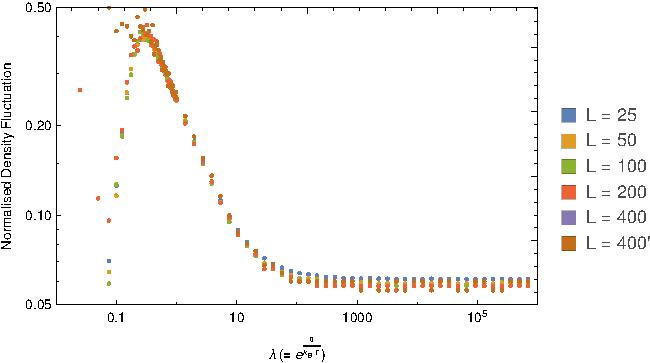
\includegraphics[width=0.95\textheight, angle=270]{numerics/images/lambdaScan/normDenFluc}
\end{center}
\end{figure}

As this causes the points to generally align for $\lambda>0.3$, this suggests that in that regime the 
dependence of $L \times \Var (\rho)$ upon $L$ is pretty weak; therefore,
the density fluctuation scales as $\mathcal{O}(L^{-1})$, implying that the number of particles in the
system fluctuates as $\mathcal{O}(1)$, which makes perfect sense when you consider that the system
allows particles to enter and leave the system only at the two boundaries, which do not change with the
system size in any sense. We also observe that there is a visible bump as we pass through the suspected
transition, but as with our higher current moments it is not a spike or discontinuity. We also
observe that for the smaller systems the fluctuation comes back under control as $\lambda$ keeps getting
smaller, whilst for larger ones the fluctuations remain large. We suggest that this is due to the fact
that we have observed the fluctuations over some timescale; thus if the system is undergoing long, slow
fluctuations over timescales longer than our observation frame, we will underestimate these fluctuations.
This is in essence a ``time to equilibration'' error, in the sense that the system's equilibration
timescale is longer than our observation timescale, and this informs us that we should be dubious about
our larger-$L$ results once we get into the extremely small $\lambda$ regime.

\subsubsection{Time-Averaged Density Profiles}
If we use the same methodology as in Sec. \ref{sec:ovDens}, but instead take long-term time averages, we can
compute the time-invariant average occupation of particular sites for a system with given $\lambda$ and boundary
conditions. In Fig. \ref{fig:densityProfiles} we show how this density profile changes with $\lambda$ for fixed 
boundary densities $(\rho_0, \rho_L) = (0.6, 0.4)$.
\begin{figure} \caption[Time-averaged density profiles for systems with fixed boundary densities, over a range of 
$\lambda$.]{Time-averaged density profiles for systems with fixed boundary densities $(\rho_0, \rho_L)=(0.6, 0.4)$, 
over a range of $\lambda$. Here the system size used is $L=100$. The top plot shows the density profile with a 
selection of $\lambda$ values coded by colour. The bottom plot shows a coloured density plot showing the continuous
variation of the time-averaged profile with $\lambda$. Note that the standard errors on these densities are very small
compared to $1$ (the maximum density), so error bars are not displayed.}
\label{fig:densityProfiles}
\begin{center}
\begin{tabular}{c} 
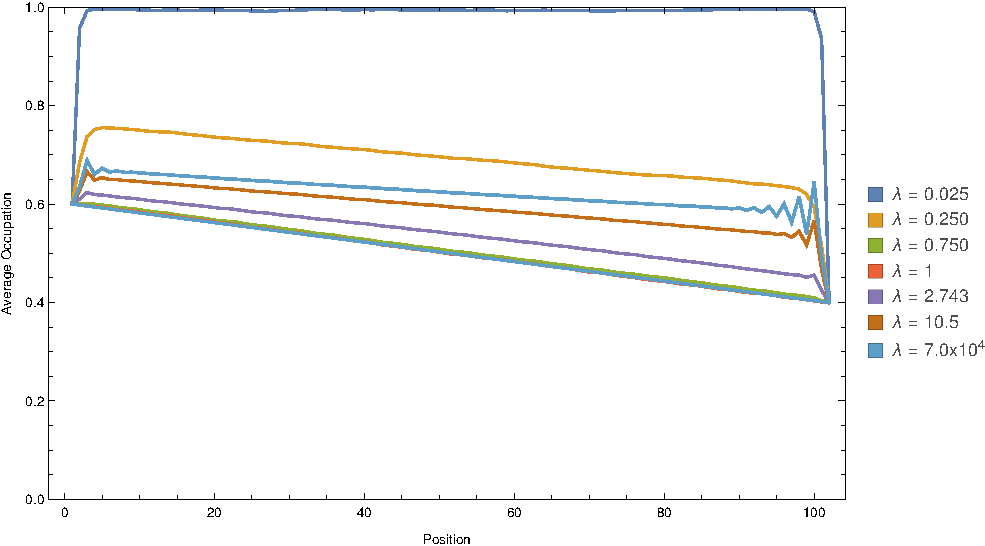
\includegraphics[width=0.9\linewidth]{numerics/images/diffCoeff/densityInstances} \\
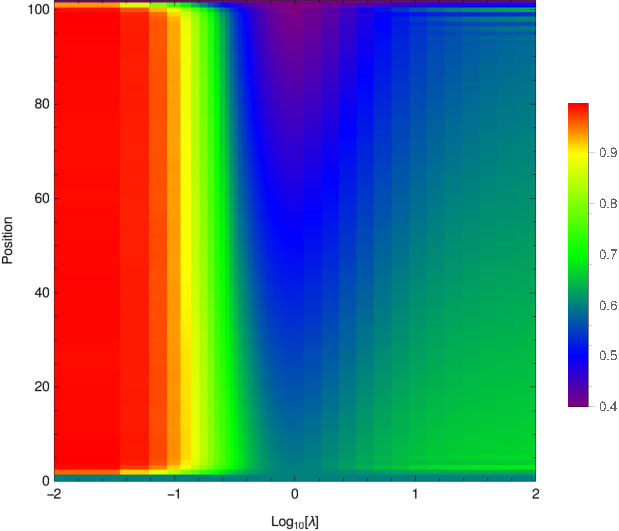
\includegraphics[width=0.9\linewidth]{numerics/images/diffCoeff/graemeDensityProfile} \\
\end{tabular}
\end{center}
\end{figure}
We see some general trends:
\begin{itemize}
 \item For $\lambda=1$ and other nearby values, the density profile is a smooth, flat descent from the high density to
 the low density.
 \item For very small $\lambda$, the system nearly fills, except for just around the boundaries (where particles
 are still quite free to move in and out of the system).
 \item For very large $\lambda$, the system adopts another flat gradient in the bulk, but this time interpolating
 between densities higher than the boundary densities we used in this case. In addition, there are also oscillations
 observed near to the boundaries. Due to the small standard errors estimated, we are quite sure that these are not
 calculational artefacts, and are in fact caused by a combination of the extremely repulsive nature of the particles
 and the order which is being imposed by the boundaries themselves. This effect is consistent with our TRM results
 displayed in Fig. \ref{fig:analDensProf}.
\end{itemize}


\subsubsection{Block Size Distribution}
The final type of measurement we have recorded in this ``$\lambda$-scan'' series of calculations is
the distribution of block sizes. By this we mean that we observe how many contiguous runs of $1$, $2$ 
and so on particles there are and add these to a time-weighted histogram, as per our method outlined in
Sec. \ref{sec:kmcLib}. If we do this, again using our run parameters from
Fig. \ref{fig:lambdaScanDensityFluc}, we find that the mean block size and its standard error vary
as shown in Fig. \ref{fig:blockSizeDistn}.
\begin{figure} \caption[The mean block size and its standard error.]{The mean block size, calculated using KMC 
with the same run parameters as we did for Fig. \ref{fig:1DlambdaScans}. Note that the error estimates here are 
plotted, and are presumably underestimates for extremely small $\lambda$.} 
\label{fig:blockSizeDistn}
\begin{center}
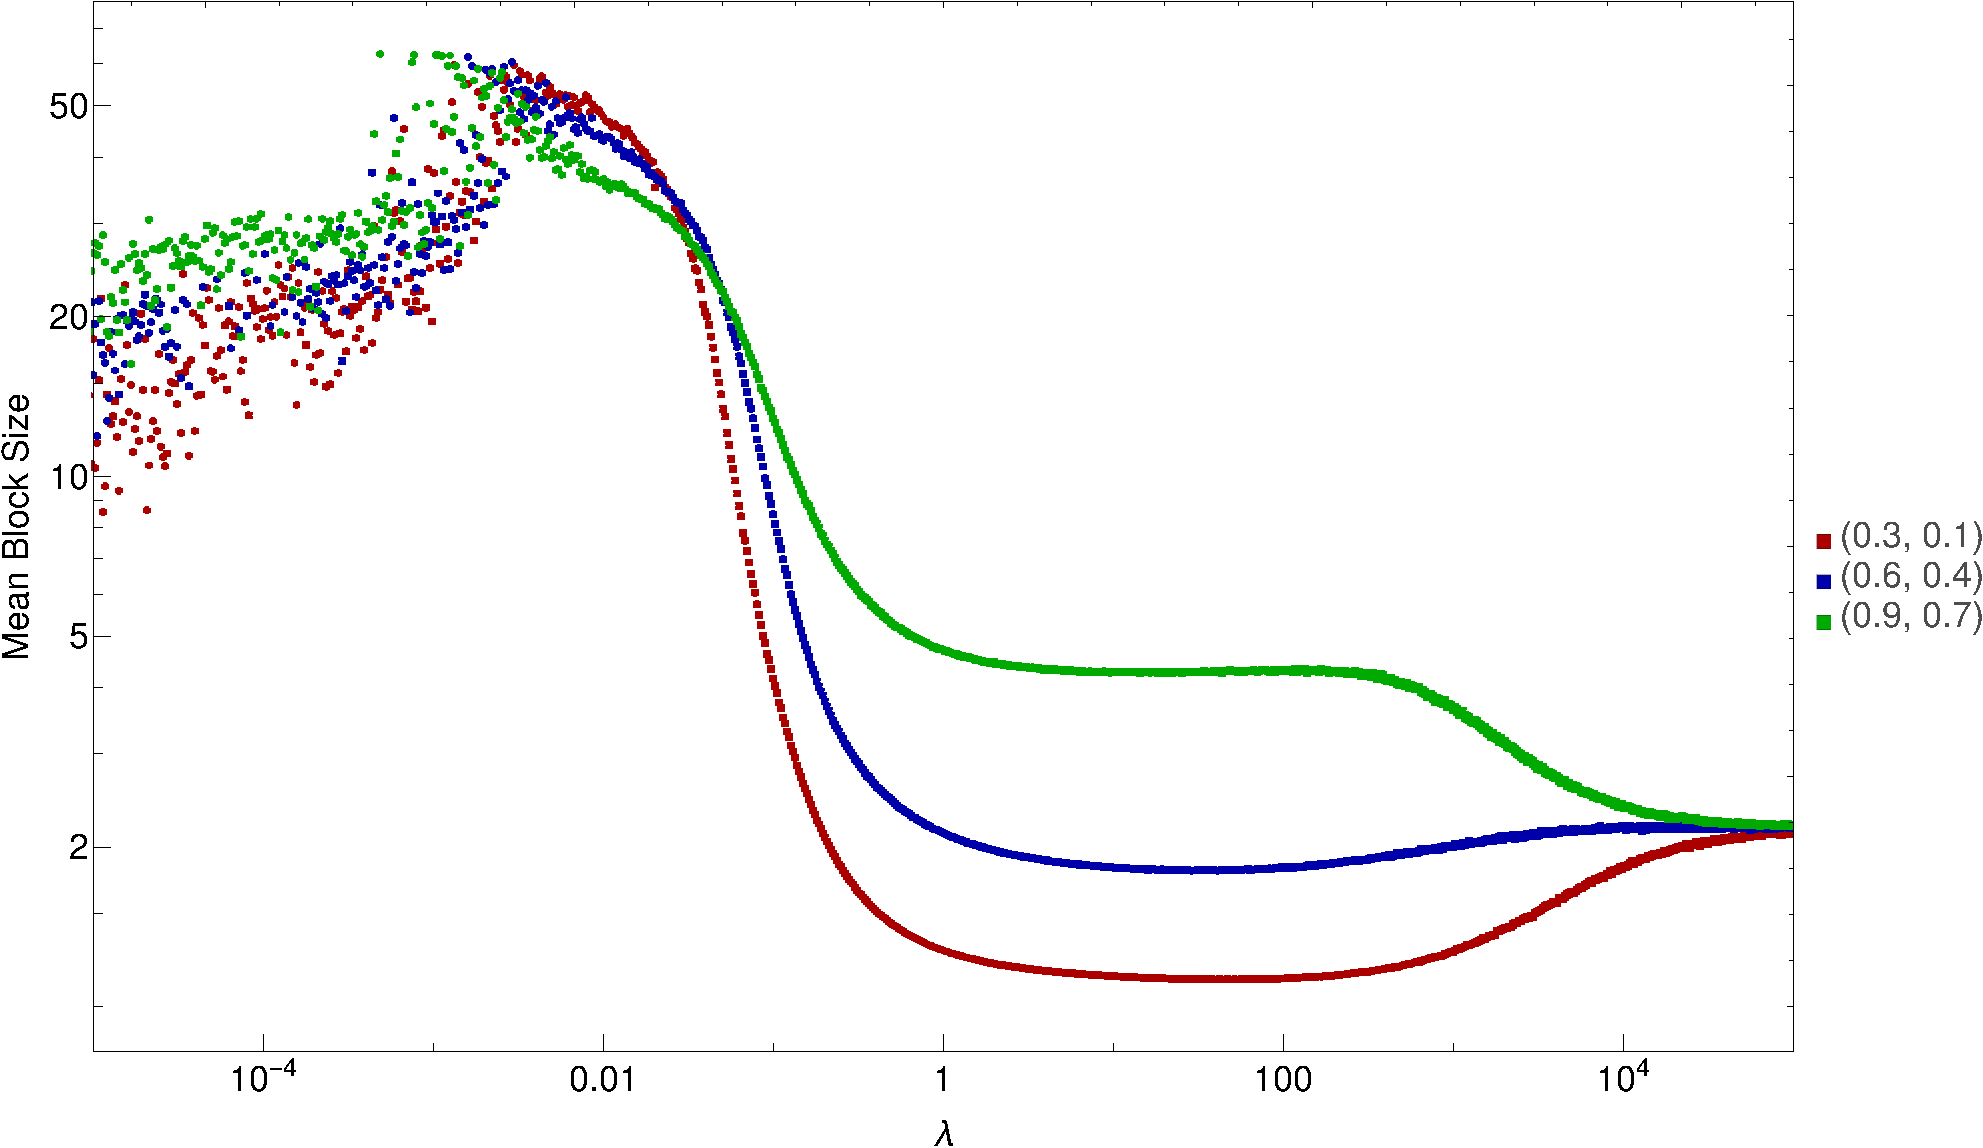
\includegraphics[width=0.95\textheight, angle=270]{numerics/images/lambdaScan/correctionBlockSizes}
\end{center}
\end{figure}

Here we once again see that we have convergence in the large-$\lambda$ limit, to an average block
size very close to $2$ which is in line with our ideas about maximal transport with a density of 
$\frac{2}{3}$. As we go towards $\lambda=1$, we find that the block size distribution reverts to
that which we'd expect by just randomly arranging particles with given densities, which is essentially
what is happening in SEP. As we go through the transition, the mean block size suddenly takes off,
whilst the fluctuation in the block size peaks, before once again starting to reduce. Once we get to 
very small $\lambda$, we lose the signal in noise, in a similar way to how we see all our results become
noise-dominated in the extremely small $\lambda$ regime.


\subsection{Varying $\lambda$ and Boundary Density Difference Together} \label{sec:constDens}
Another type of calculation we can perform is one in which we hold the average of the boundary 
densities constant, whilst varying their difference and $\lambda$; we can do this by using boundary
conditions $(\rho_0, \rho_L)=(\rho + \frac{1}{2} \delta \rho , \rho - \frac{1}{2} \delta \rho)$ and 
varying $\delta \rho$ whilst keeping $\rho$ constant. In our calculations
of this style, we set $\rho=\frac{1}{2}$, $L=64$, performed $400000$ 
equilibration steps and then $1000$ alternating measurement and relaxation
runs of $16000$ and $1000$ steps respectively. From this we calculated
the same kinds of quantities as in Sec. \ref{sec:lambdaScans}; the 
principle results are displayed in Fig~\ref{fig:constDens}.
\begin{figure} \caption[Results obtained by fixing the average of the boundary densities and varying their difference and $\lambda$]{The main results obtained 
when we have boundary densities 
$(\rho_0, \rho_L)=(\rho + \frac{1}{2} \delta \rho , \rho - \frac{1}{2} \delta \rho)$ and vary $\lambda$ and $\delta \rho$.
Here $\rho=\frac{1}{2}$. Clockwise from top left, we have: The mean current, the current variance,
the mean block size, and the mean overall system density. Note that in our mean block size
computation, many calculations failed; this explains the sparsity of the data in the right
of the image.} 
\label{fig:constDens}
\begin{center}
\begin{tabular}{c c} 
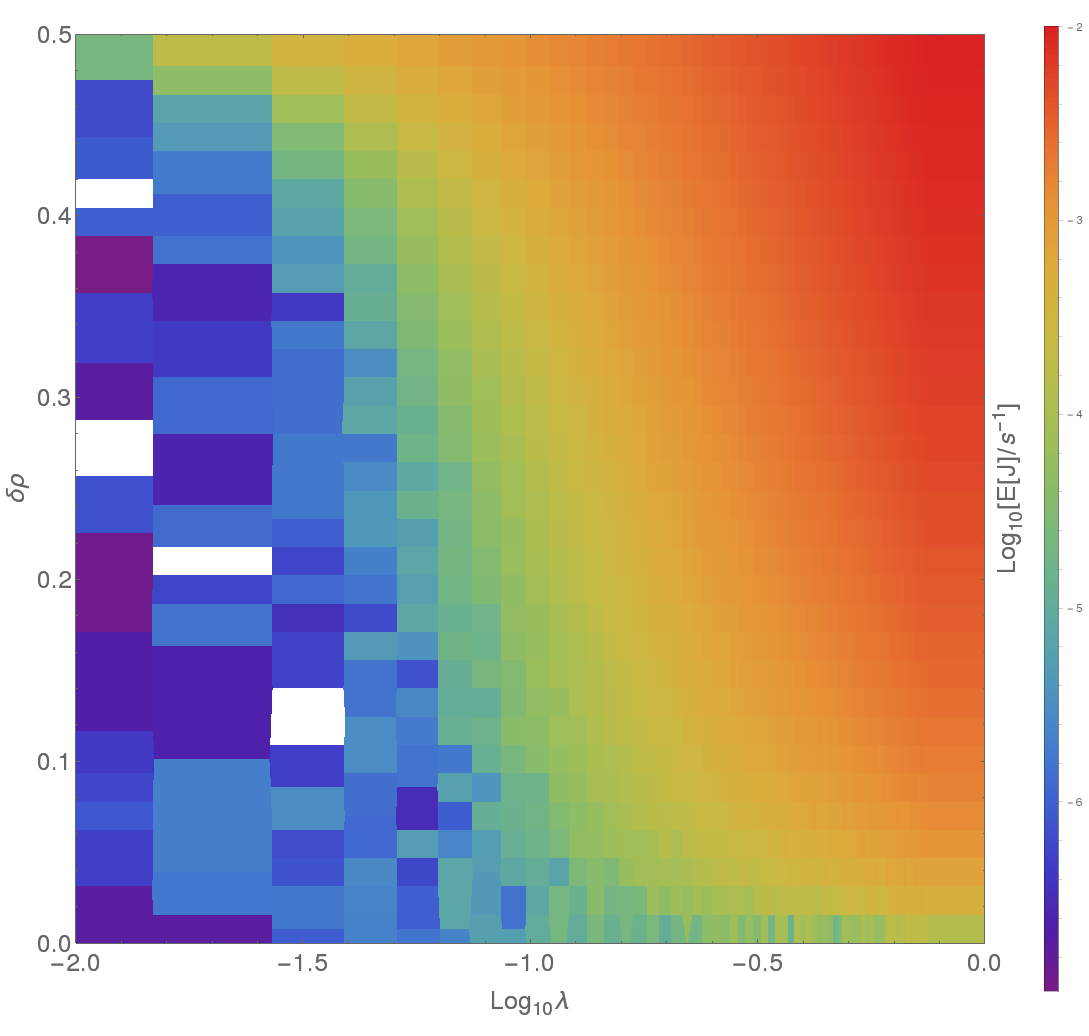
\includegraphics[width=0.49\linewidth]{numerics/images/lambdaConcDiff/current} & 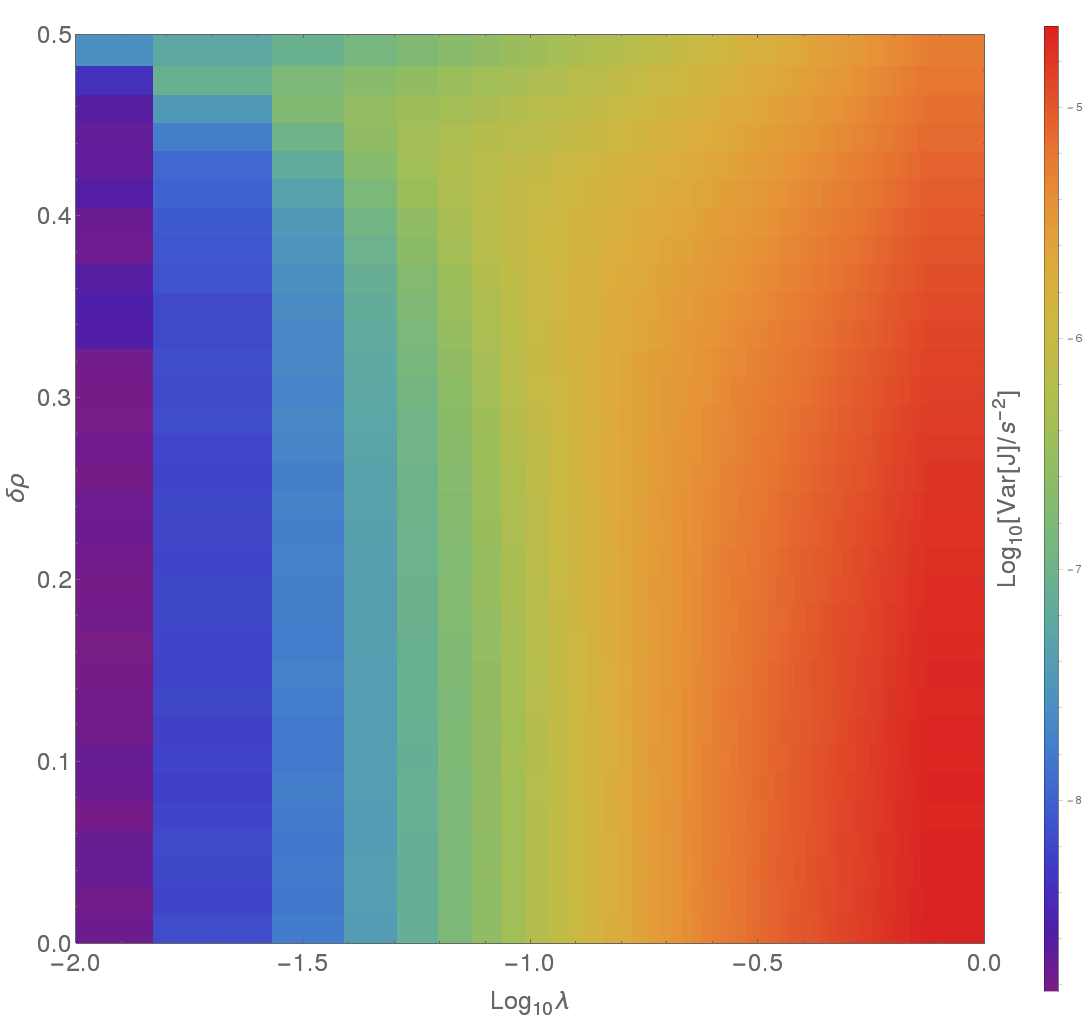
\includegraphics[width=0.49\linewidth]{numerics/images/lambdaConcDiff/currentVar} \\
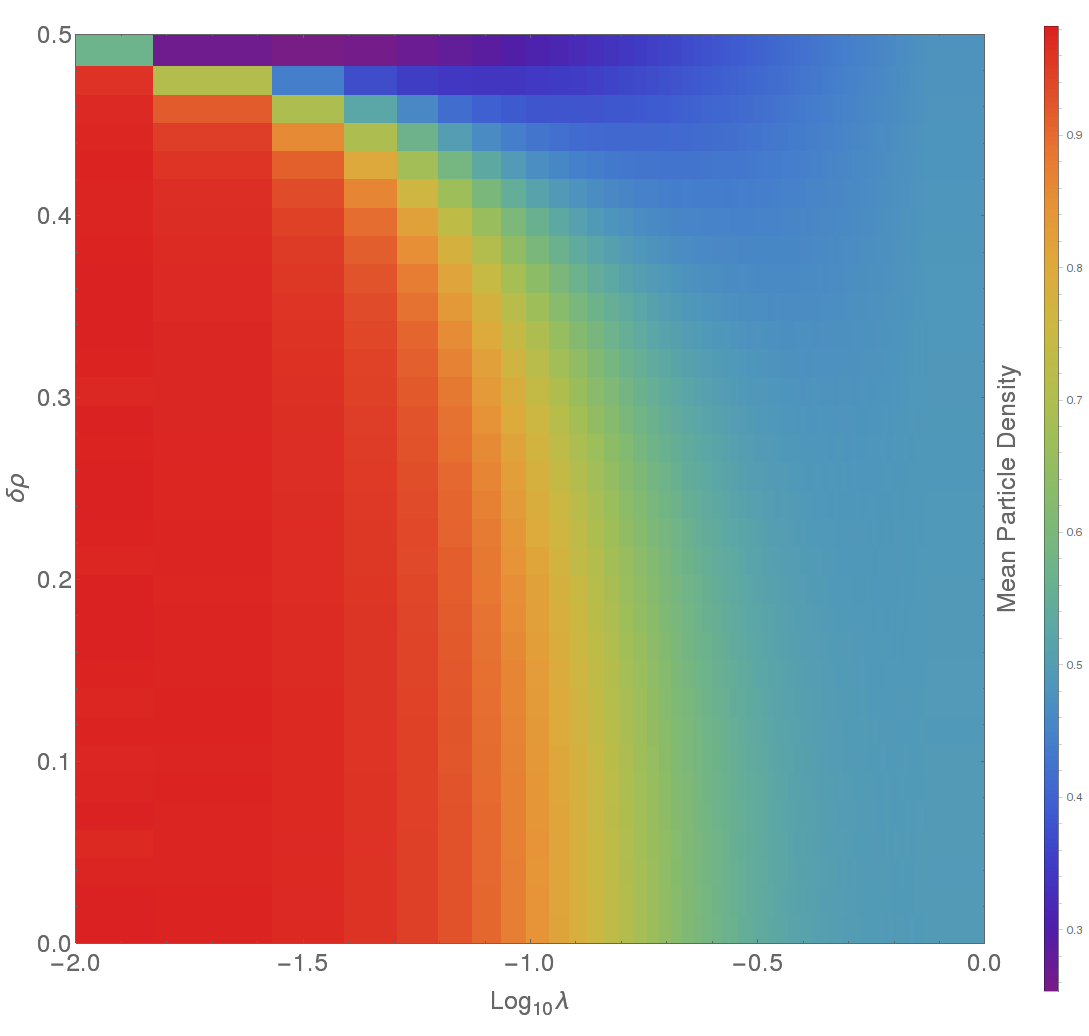
\includegraphics[width=0.49\linewidth]{numerics/images/lambdaConcDiff/density} &
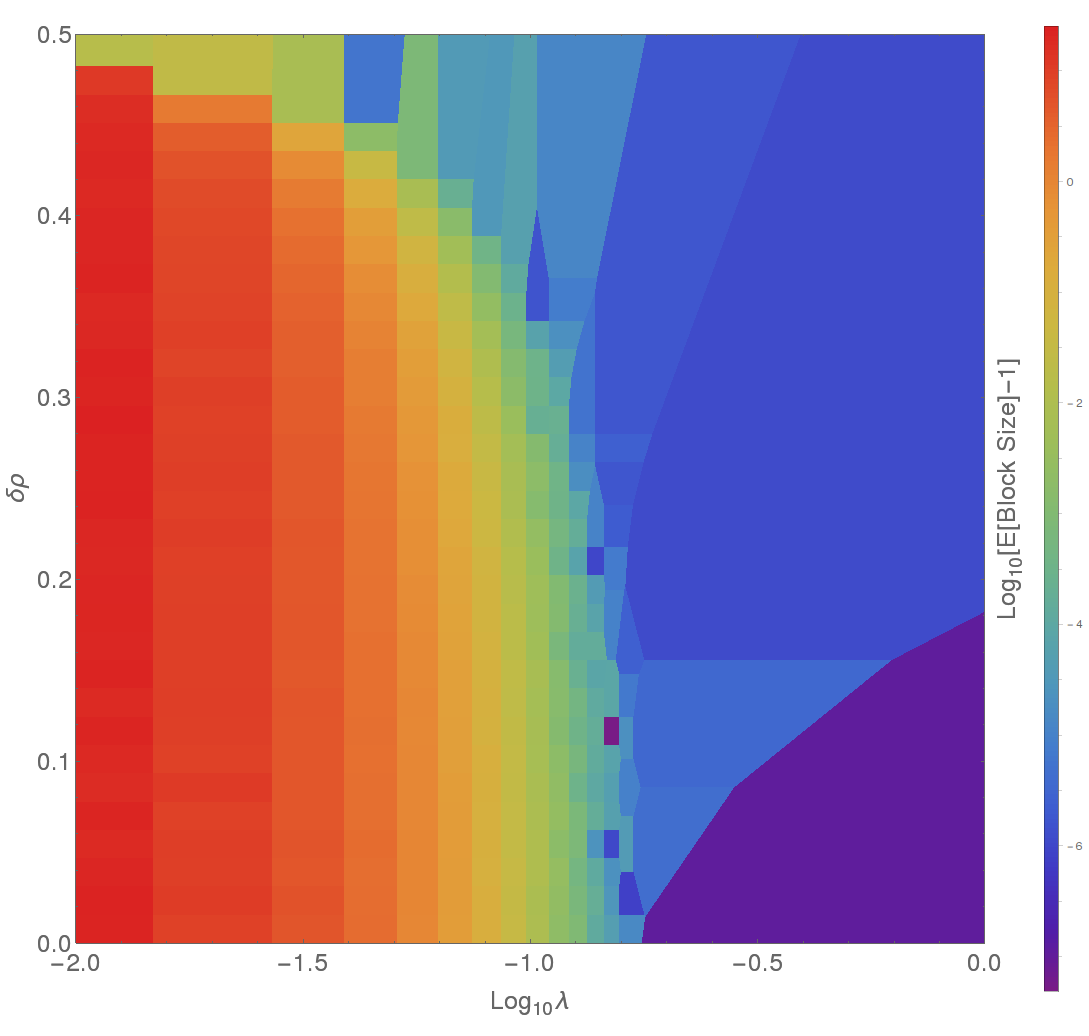
\includegraphics[width=0.49\linewidth]{numerics/images/lambdaConcDiff/blockSize} \\
\end{tabular}
\end{center}
\end{figure}

In each of these results, we see that we essentially partition the domain into two regimes:
small $\lambda$ with small $\delta \rho$, and another regime where $\lambda$ is larger, or 
$\delta \rho$ is bigger. In other words, when $\lambda$ becomes small the system gains density,
block size, and flow slows; however, a large boundary difference can still force through current
and keep density and block size lower, so there is a tradeoff between these competing forces.

\subsection{Varying the Boundary Densities with Constant $\lambda$}
Instead of varying $\lambda$, we can instead choose to hold it constant whilst we vary the two
boundary densities. We have done this with a series of different $\lambda$; the mean current results
are displayed in Fig. \ref{fig:boundaryVarCurr}, and the mean densities displayed in 
Fig. \ref{fig:boundaryVarDens}. Here we used $L=124$, with $160000000$ equilibration steps and then
$1000$ sets of analysis runs of $1600000$ KMC steps interspersed with relaxation runs of 
$1000$ steps.
\begin{figure} \caption[Mean currents observed when varying the boundary densities, fixing $\lambda$,
for different $\lambda$]{Here we have varied $\rho_0$ and $\rho_L$ separately for several different 
values of $\lambda$, and measured the resulting mean current. Note that here we have plotted the 
absolute value of the current, as it should be antisymmetric about $\rho_0 = \rho_L$, which would
not take kindly to having its logarithm taken. White patches indicate measurements
which are out of bounds, generally because they were too large, whose
incorporation would have negatively affected the usefulness of the graph.} 
\label{fig:boundaryVarCurr}
\begin{center}
\begin{tabular}{c c} 
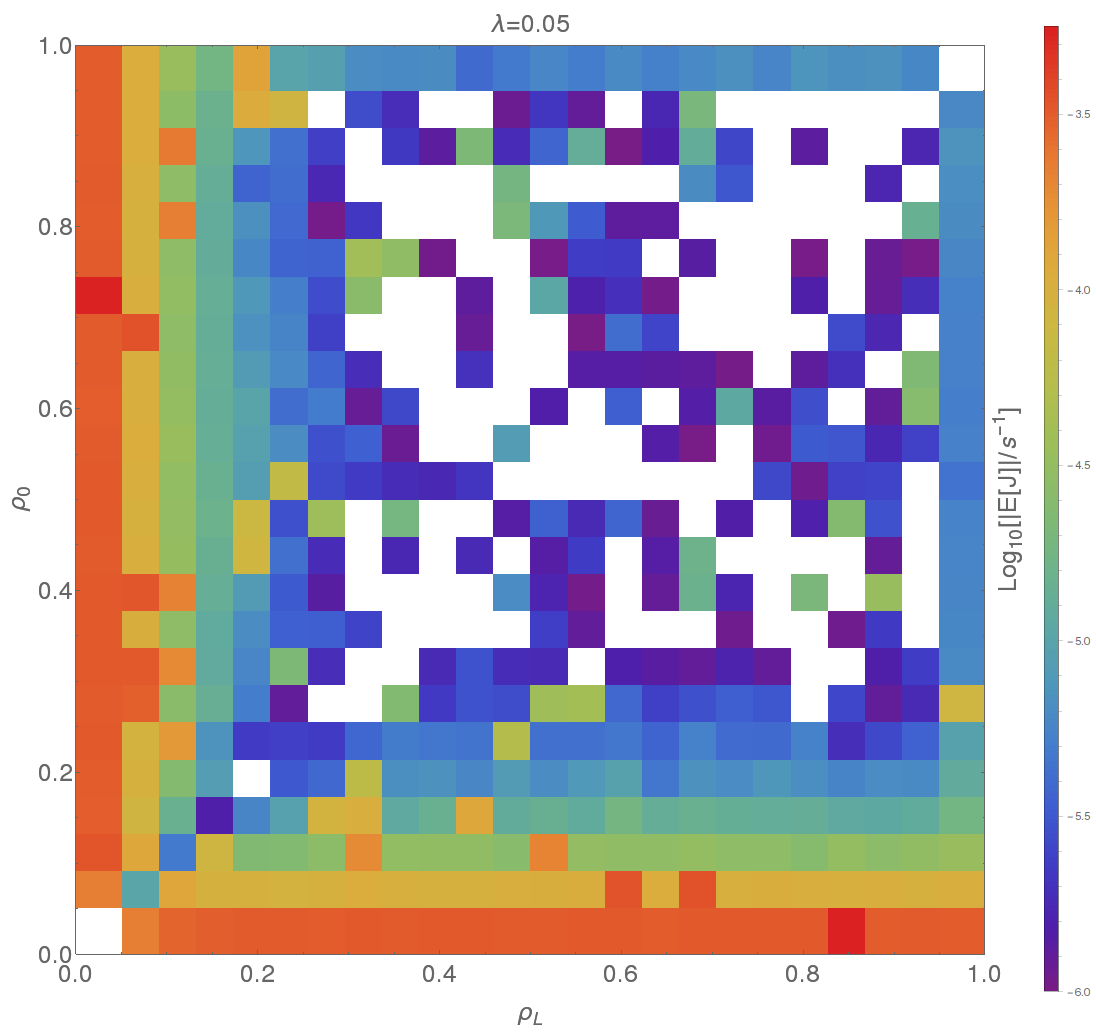
\includegraphics[width=0.45\linewidth]{numerics/images/concFrames/concDataCurr0p05.png} &
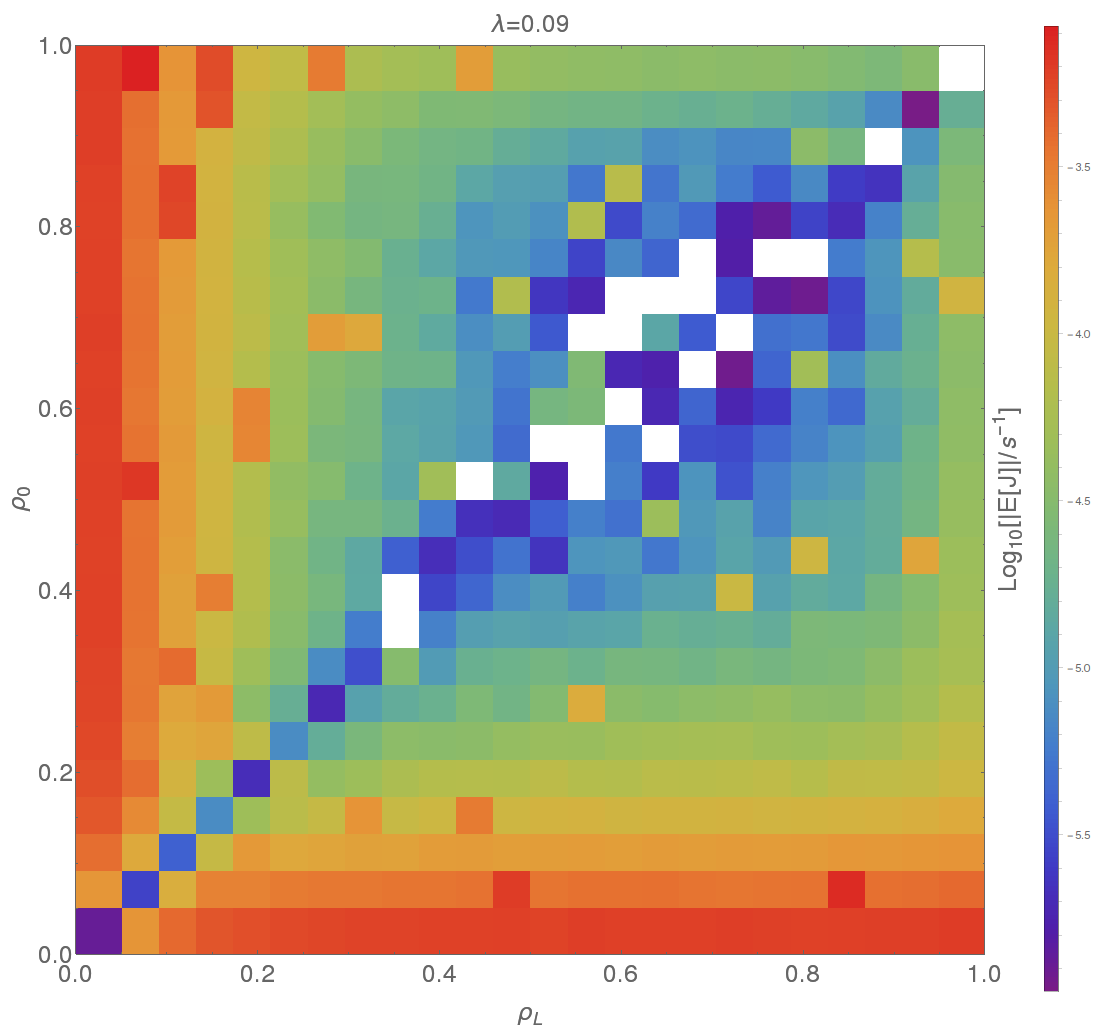
\includegraphics[width=0.45\linewidth]{numerics/images/concFrames/concDataCurr0p09.png} \\
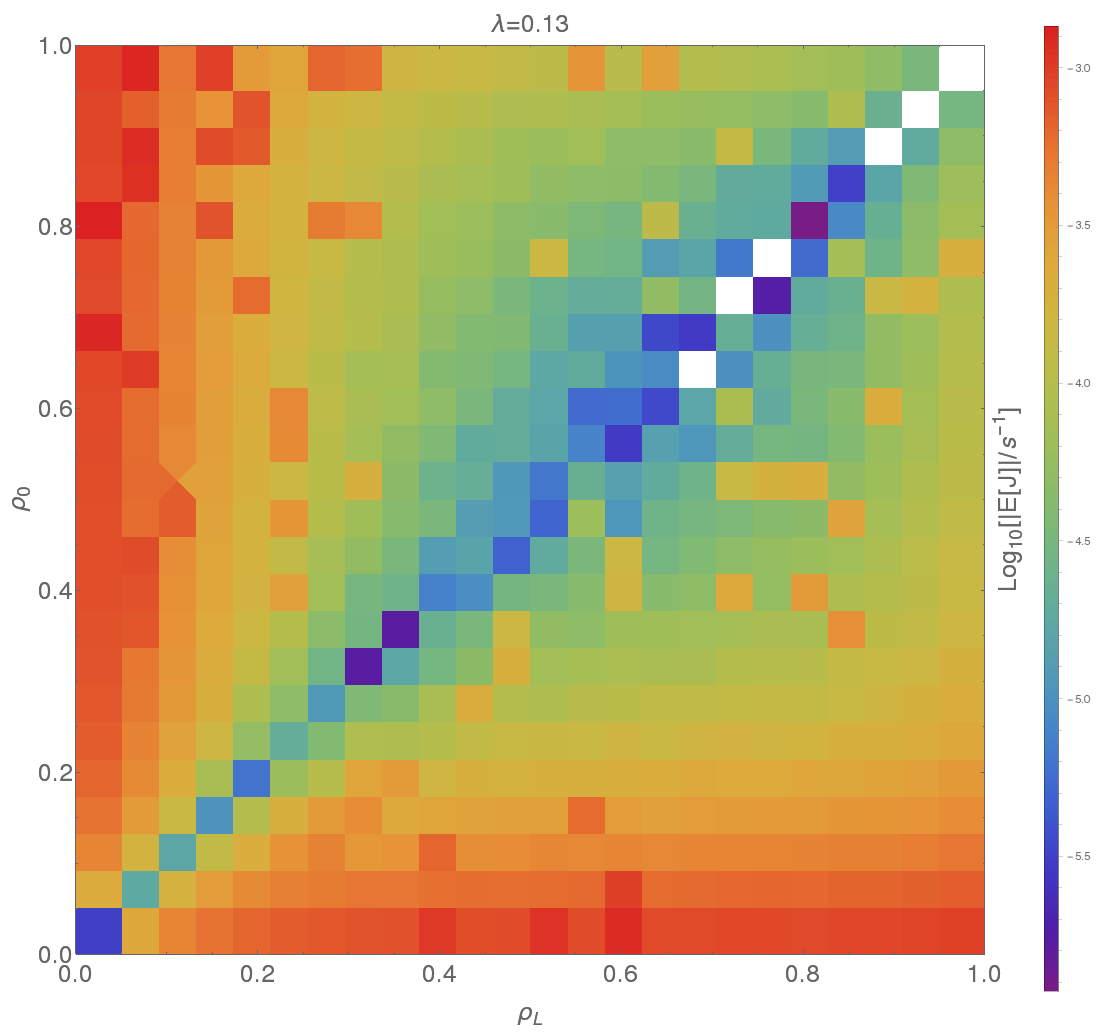
\includegraphics[width=0.45\linewidth]{numerics/images/concFrames/concDataCurr0p13.png} & 
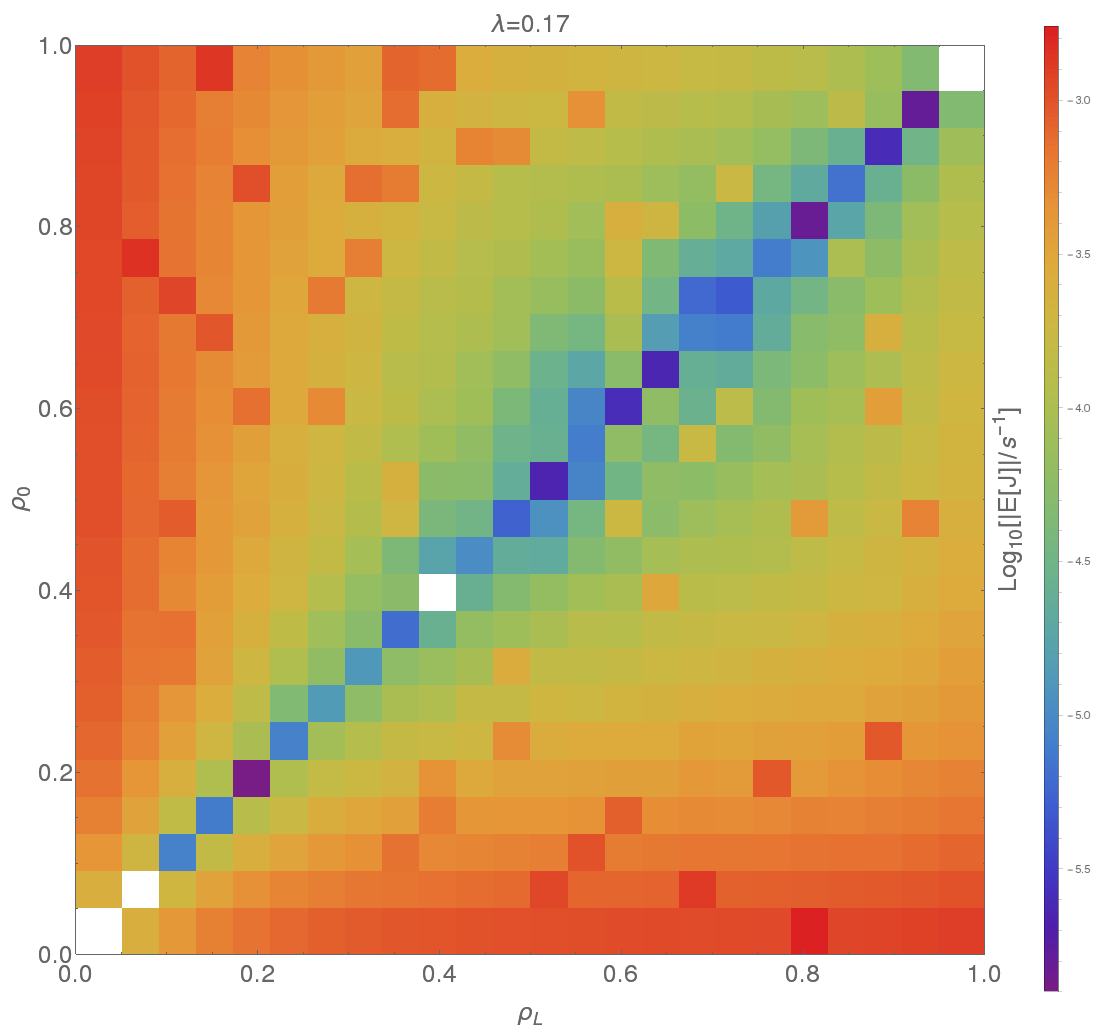
\includegraphics[width=0.45\linewidth]{numerics/images/concFrames/concDataCurr0p17.png} \\
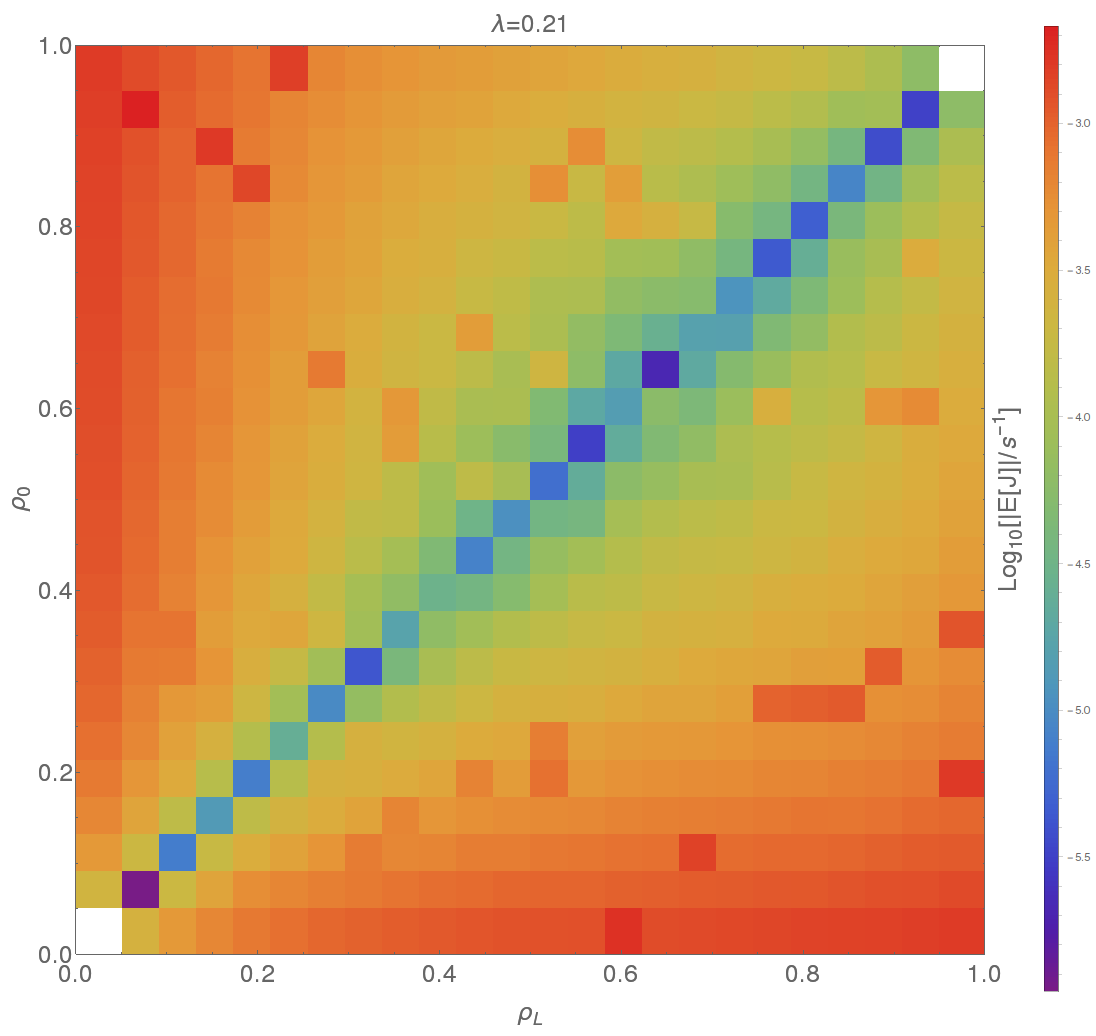
\includegraphics[width=0.45\linewidth]{numerics/images/concFrames/concDataCurr0p21.png} &
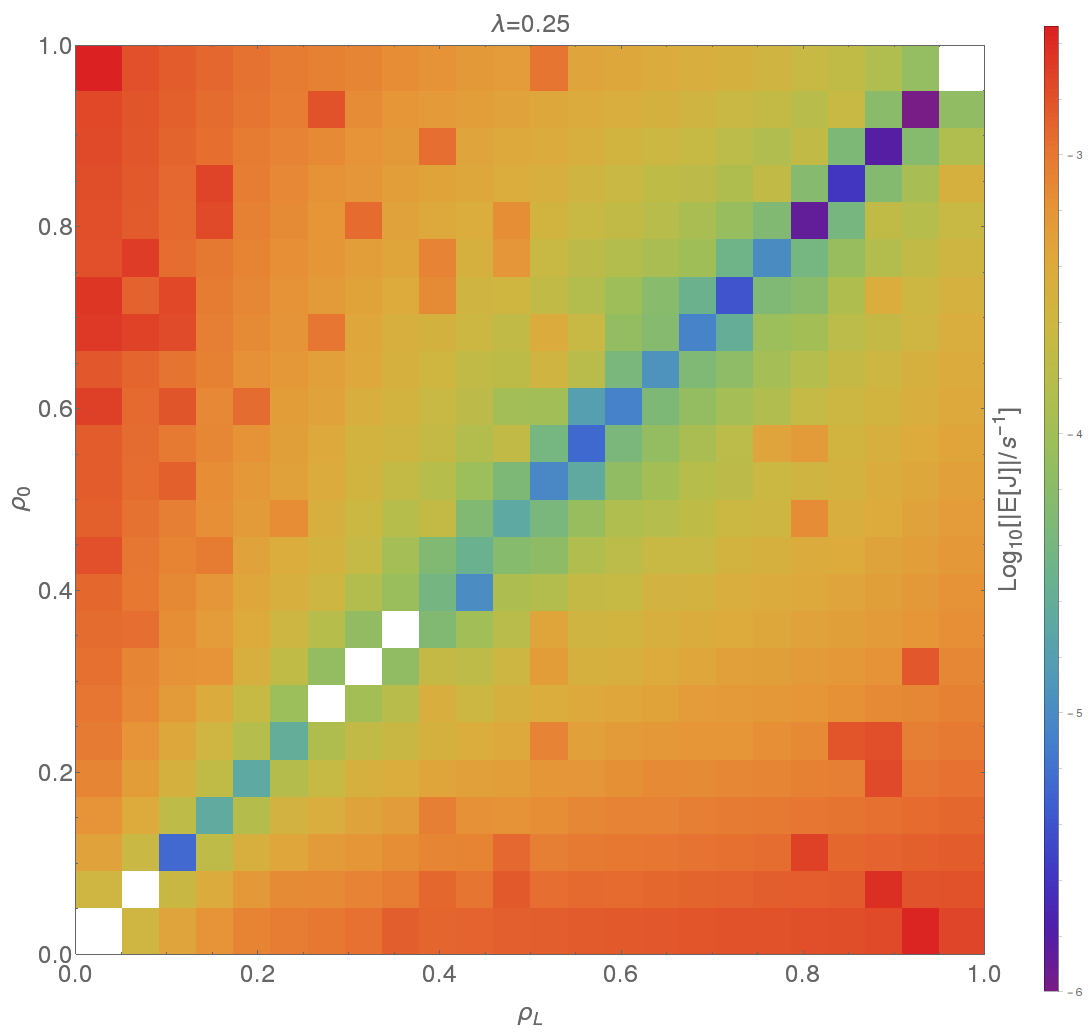
\includegraphics[width=0.45\linewidth]{numerics/images/concFrames/concDataCurr0p25.png} \\
\end{tabular}
\end{center}
\end{figure}
\begin{figure} \caption[Mean densities observed when varying the boundary densities, fixing $\lambda$,
for different $\lambda$]{As Fig. \ref{fig:boundaryVarCurr}, only this time we have plotted the mean 
densities instead of the currents.} 
\label{fig:boundaryVarDens}
\begin{center}
\begin{tabular}{c c} 
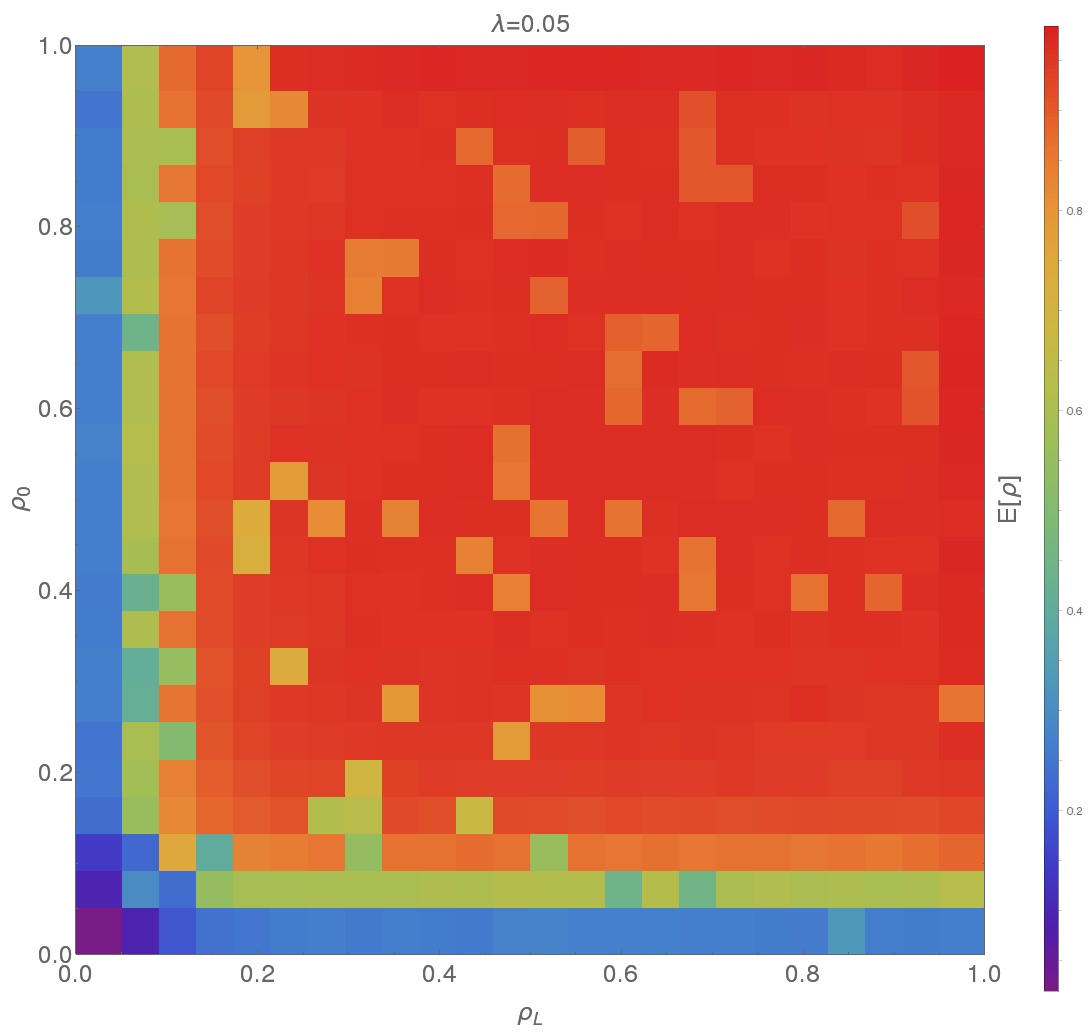
\includegraphics[width=0.45\linewidth]{numerics/images/concFrames/concDataDens0p05.png} &
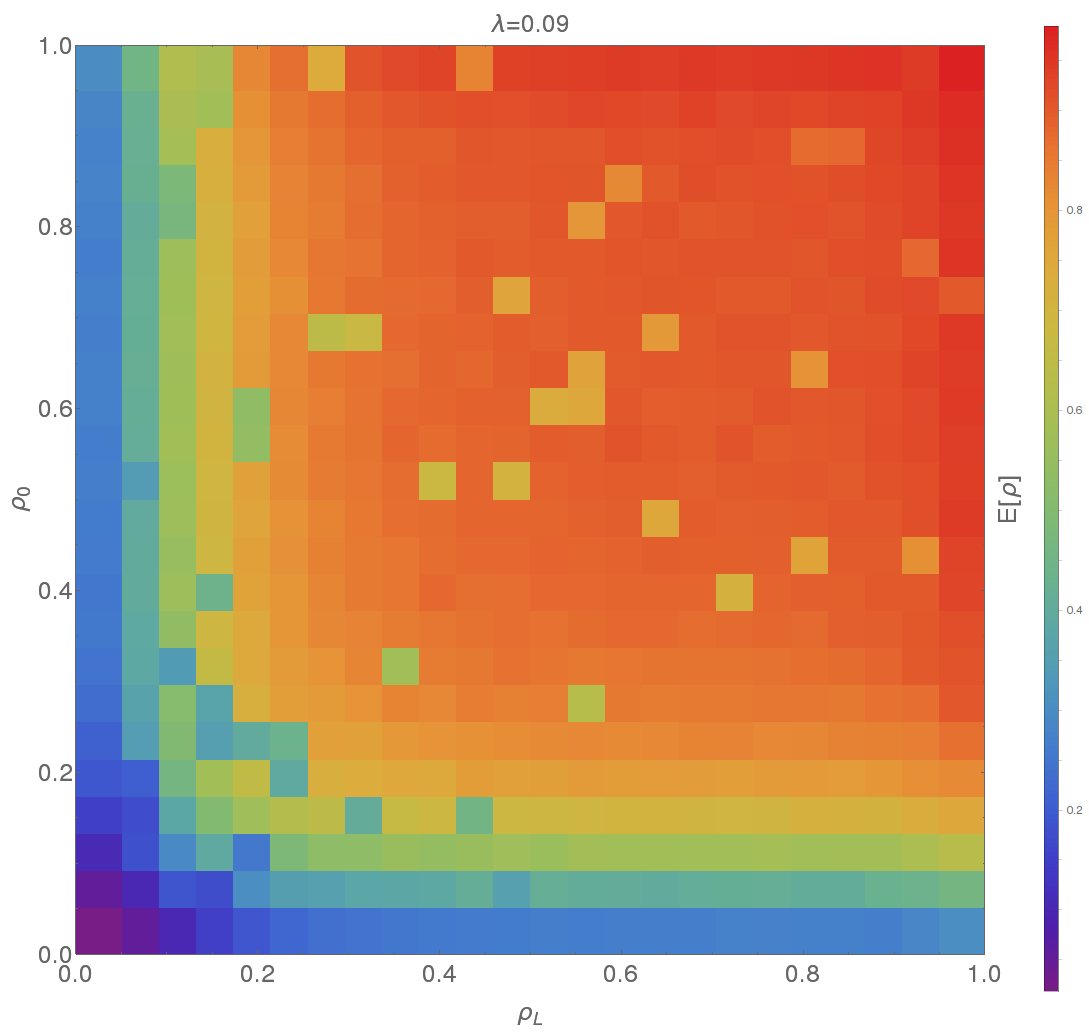
\includegraphics[width=0.45\linewidth]{numerics/images/concFrames/concDataDens0p09.png} \\
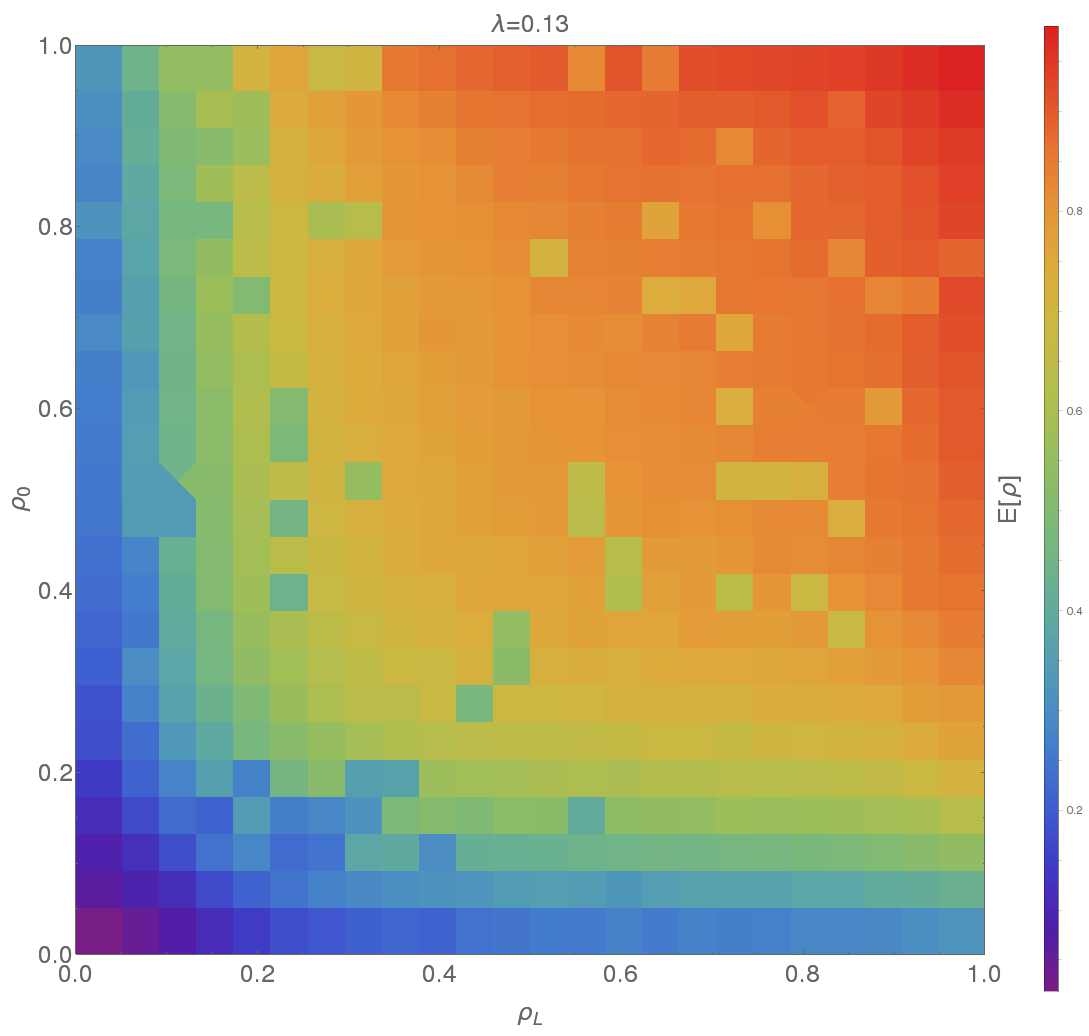
\includegraphics[width=0.45\linewidth]{numerics/images/concFrames/concDataDens0p13.png} & 
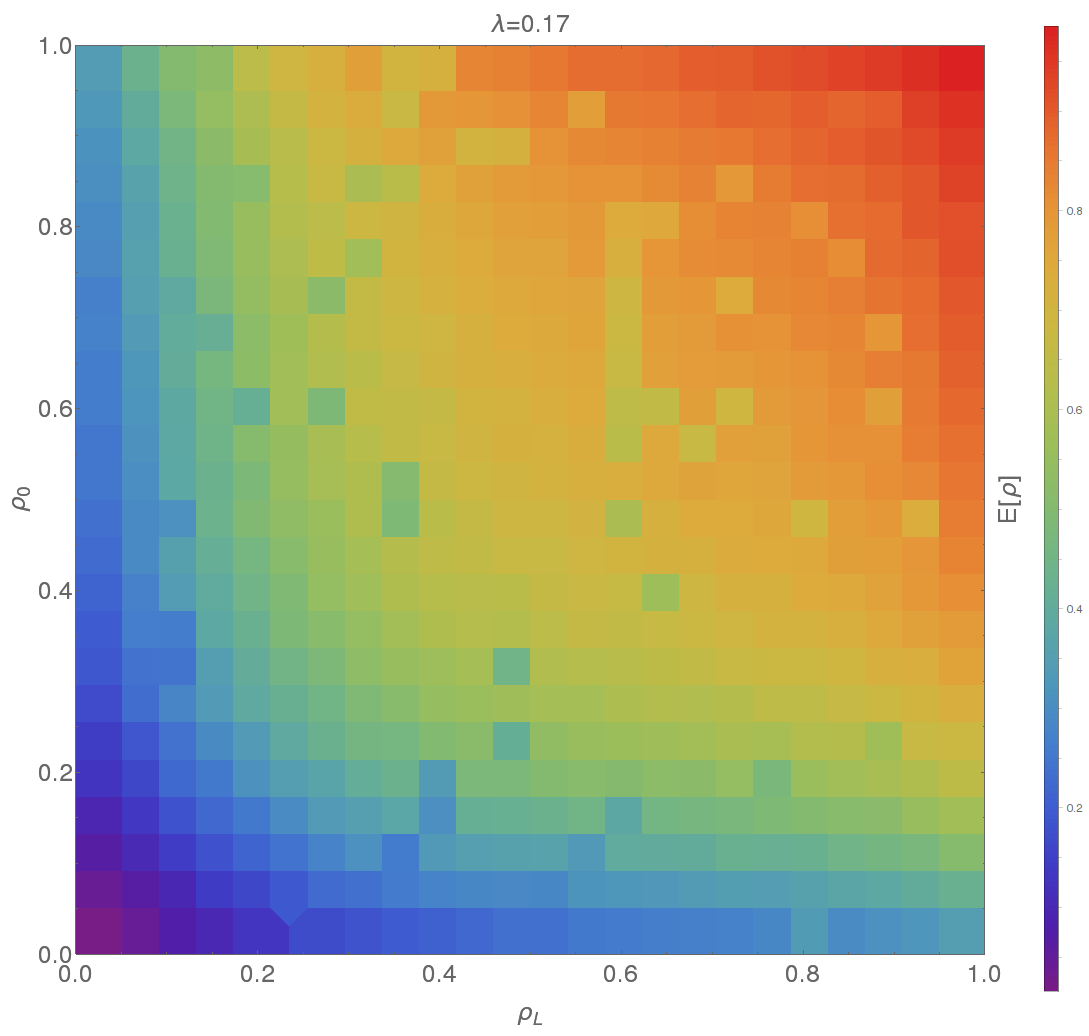
\includegraphics[width=0.45\linewidth]{numerics/images/concFrames/concDataDens0p17.png} \\
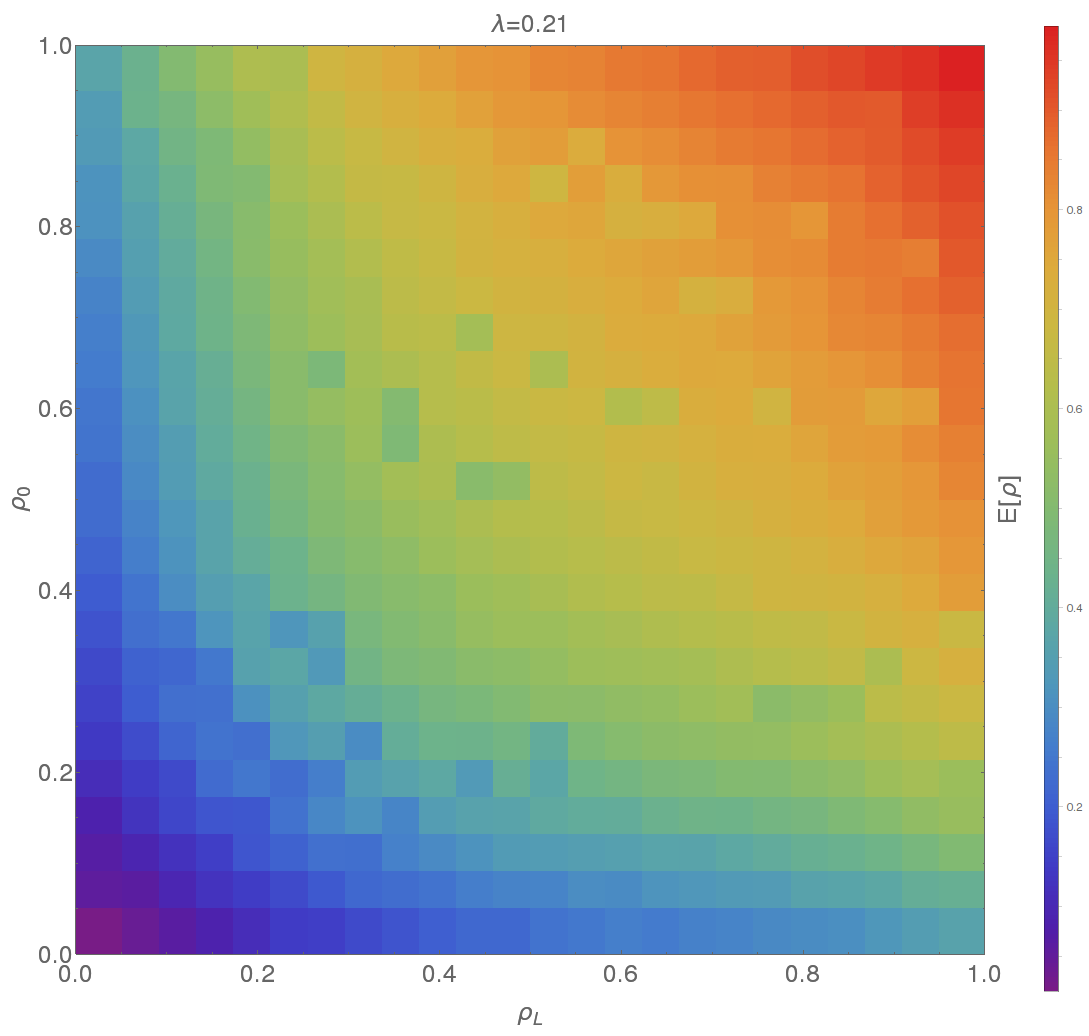
\includegraphics[width=0.45\linewidth]{numerics/images/concFrames/concDataDens0p21.png} &
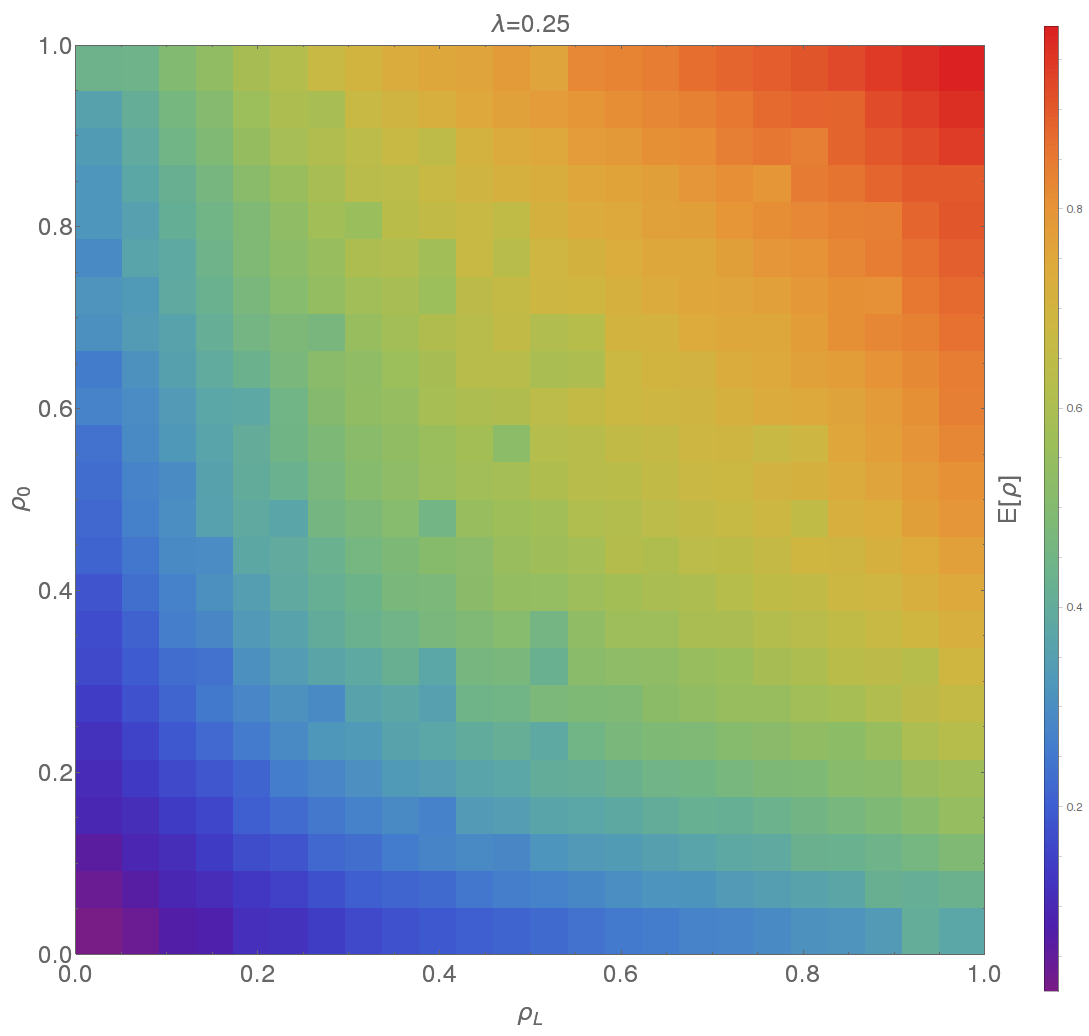
\includegraphics[width=0.45\linewidth]{numerics/images/concFrames/concDataDens0p25.png} \\
\end{tabular}
\end{center}
\end{figure}

We see a similar picture to the one we saw in Sec. \ref{sec:constDens}; the system naturally 
wishes to relax to a high-density, low-current regime at small $\lambda$ regardless of boundary 
conditions, (probably primarily due to attempts to minimise free energy), but this is suppressed by
large boundary density differences. It is also important to note that Fick's Law is violated in every case here,
as one can see by the fact that the colour gradients are not constant along lines of constant $\rho_0 + \rho_L$.

\subsection{Diffusion Coefficient}
Wrapping up our calculations in $1$D, we can compute the effective diffusion coefficient, which
can be compared with our existing calculation in Sec. \ref{sec:TRMDensityCurrent} (see 
Fig. \ref{fig:TRMDiffCoeff} specifically for graphical comparison). To do this, we perform
calculations with boundary densities $(\rho_0, \rho_L)=(\rho + \frac{1}{2} \delta \rho , \rho -
\frac{1}{2} \delta \rho)$, where we vary $\rho$, $\lambda$ and $\delta \rho$ simultaneously, and
we deliberately keep $\delta \rho$ small, in the hope that the dependency of the current upon $\delta
\rho$ is roughly linear in that regime, so that $J = \frac{\delta \rho}{L} D(\rho, \lambda)
+ \mathcal{O}(\delta \rho^2)$. Given that we have an error estimate for $J$ due to repeat runs,
we can use weighted least squares fitting to estimate the value of $D(\rho, \lambda)$, and also
its error. We did this, using $16$ values of $\delta \rho$ for each $(\rho, \lambda)$ pair we
computed (arranged in a $24 \times 12$ grid); each computation consisted of a $160000000$ KMC step
equilibration run, followed by $10$ alternating $80000000$ step measurement run and $16000000$ step
relaxation run pairs. The system size used in this case was $L=124$. Our estimates for $D$ and its
standard error are displayed in
Fig. \ref{fig:KMCDiffCoeff}. Additionally, we performed similar calculations with a wider range of 
$\lambda$ and different system sizes, which are displayed in Fig. \ref{fig:KMCDiffCoeffAltTake}.
\begin{figure} \caption[The variation of the KMC-calculated diffusion coefficient with $\rho$ and 
$\lambda$.]{The variation of the KMC-calculated diffusion coefficient with $\rho$ and 
$\lambda$. The top panel is the estimate of $D(\rho, \lambda)$, and the bottom panel is the associated
standard error.} 
\label{fig:KMCDiffCoeff}
\begin{center}
\begin{tabular}{c}
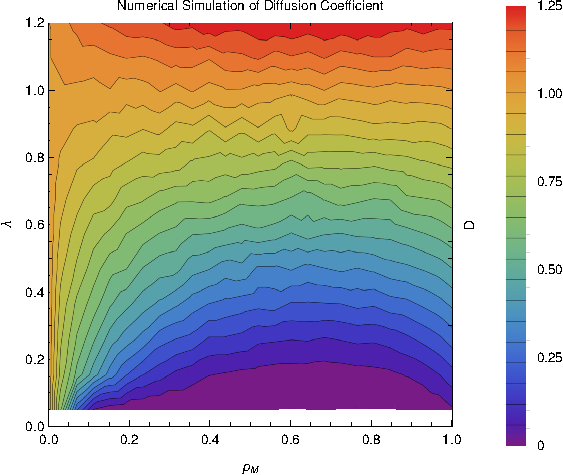
\includegraphics[width=0.9\textwidth]{numerics/images/diffCoeff/numDiffCoeff} \\
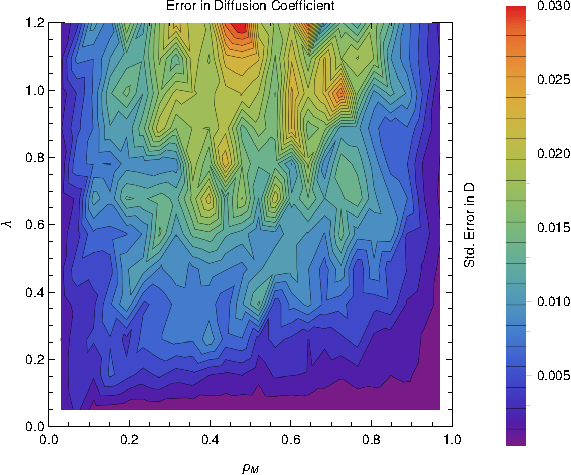
\includegraphics[width=0.9\textwidth]{numerics/images/diffCoeff/newFlowErr} \\
\end{tabular}
\end{center}
\end{figure}

\begin{figure} \caption[The variation of the KMC-calculated diffusion coefficient with $\rho$ and 
$\lambda$; alternate plots.]{Data computed using the same methodology as in Fig. \ref{fig:KMCDiffCoeff}, but this time we
have plotted the 
diffusion coefficient as a function of density with multiple coloured datasets indicating different values for 
$\lambda$. In addition, these results were made using different system sizes, with \textbf{circles}, \textbf{squares}
and \textbf{triangles} corresponding to systems of size $L=32$, $64$ and $128$ respectively.
The MFT prediction is also displayed for each $\lambda$ as a solid coloured curve. We have split the data
between low and high $\lambda$-values for ease of visualisation. } 
\label{fig:KMCDiffCoeffAltTake}
\begin{center}
\begin{tabular}{c}
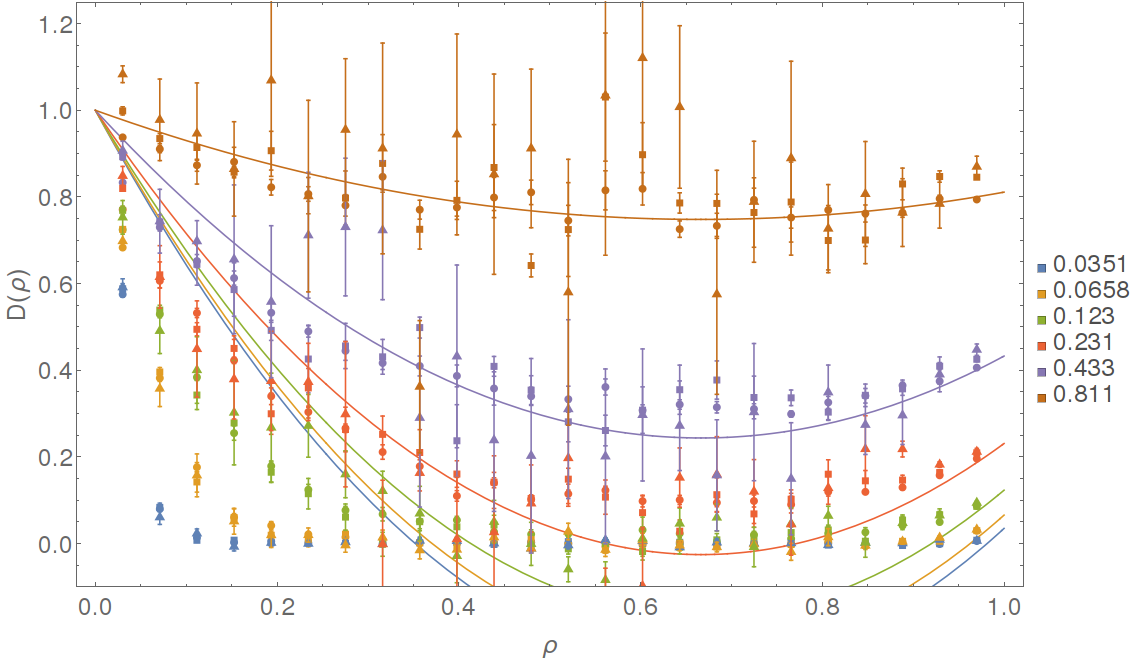
\includegraphics[width=0.95\textwidth]{numerics/images/diffCoeff/diffCoeffLow} \\
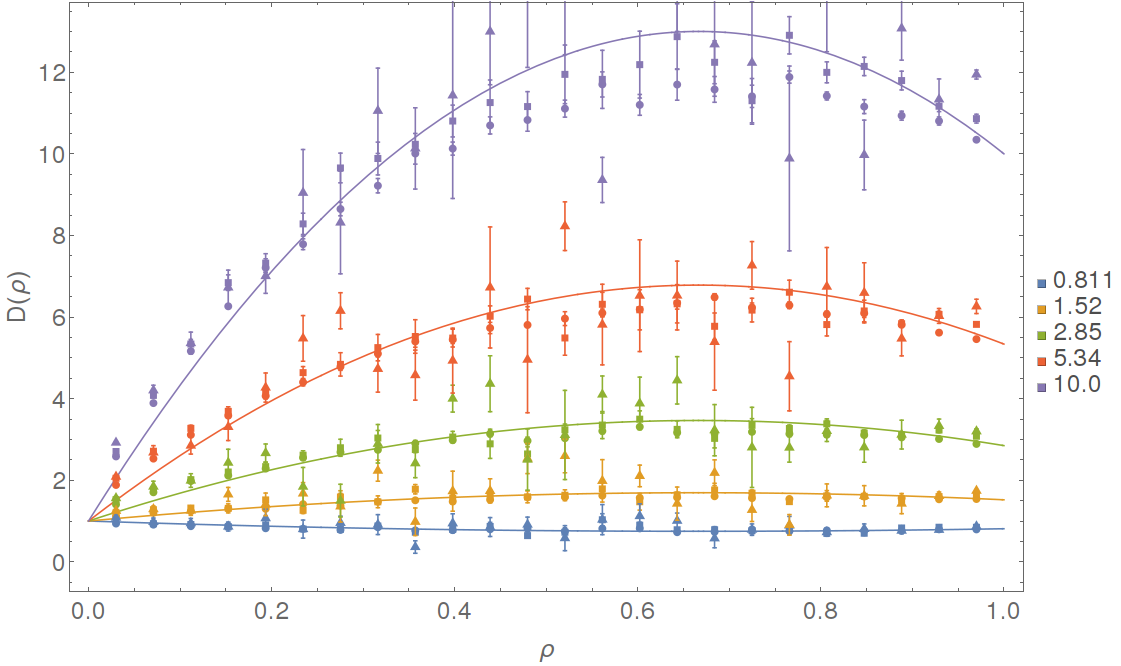
\includegraphics[width=0.95\textwidth]{numerics/images/diffCoeff/diffCoeffHigh} \\
\end{tabular}
\end{center}
\end{figure}

Please note that whilst this is probably the largest single calculation we have performed during the 
course of this research, it is also the earliest chronologically; thus, there are many issues
with it:
\begin{itemize}
 \item We probably used a system that was unnecessarily large. A size $64$ system proved to be quite adequate
 later on, and equilibrates much faster.
 \item We should have performed a larger number of shorter analysis runs; that way we would
 probably obtain a more robust estimate for $D$, which wouldn't be so susceptible to being
 kicked around by individual rogue measurements.
 \item We only hit upon the idea of scanning in $\log \lambda$ instead of $\lambda$ later on
 in the research; thus, the format here does not allow for easy direct comparison with our TRM
 results which do use $\log \lambda$. 
\end{itemize}
That said, these results do compare nicely with our MFT calculations, displayed in 
Fig. \ref{fig:diffCoeffDensityPlot}. The qualitative features are very similar, although the
MFT-predicted ``transition'' doesn't occur quite where it suggests, which we have seen  
more clearly in our scans in Sec. \ref{sec:lambdaScans}. Also, the diffusion coefficient does not seem to vary in a consistent way with system size.





\section{2D Calculation Results}
As we saw in Sec. \ref{sec:highDimSPM}, it is possible to define a logical extension of the SPM
to dimensions higher than $1$D. Whilst it is not viable to perform TRM calculations in higher 
dimensions (as the scaling with system size is already very bad), it is relatively easy to adapt
our $1$D KMC codes to perform SPM calculations in $2$D or $3$D. Such a KMC input script may be found
in \texttt{kmc/2d/2dSteadyFlow.py} in ~\cite{hellier2019a}.
One thing that does need considering in this case is that a 2-dimensional square
lattice-based domain would normally have $4$ boundaries instead of $2$, which would mean $2$ extra
boundary conditions which would need to be prescribed in addition to $\rho_0$ and $\rho_L$.
However, we have avoided this difficult by making one of the coordinates cyclic; therefore, in our
$2$D calculations we are really considering flow down a tube, with circumference $W$. We still
use the same double-layered boundary technique as in $1$D, thus for a system of length $L$
we have $W \times (L+4)$ lattice sites in play.

\subsection{Aspect Ratio Considerations} \label{sec:aspectRatio}
Given that we now have two system size variables to play with, a natural question to ask would be
how the system's behaviour changes as we adjust $W$ and $L$, and in particular their aspect ratio.
We would expect that total current with given boundary conditions would usually scale inversely with
$L$ and in proportion to $W$ (as more current can flow across a wider cyclic surface); thus, the
total current should scale as $\frac{W}{L}$, the aspect ratio of the system. We can test this, and
also check how system convergence scales with system size, by performing calculations of the current
with several different $(L, W)$ pairs. We have maintained the boundary conditions to be 
$(\rho_0, \rho_L) = (0.75, 0.25)$ throughout, and in each case used an initial equilibration run of
$1600000$
KMC steps followed by $4096$ runs consisting of alternating $16000$-step and $320000$-step
analysis and relaxation runs respectively; then, we have varied $\lambda$ and measured the mean
current. The results are displayed in Fig~\ref{fig:aspectRatios}.
\begin{figure} \caption[The variation of the current in a $2$D SPM system with $\lambda$,
for a variety of different system sizes and aspect ratios.]{The variation of the current in a $2$D SPM
system with $\lambda$, for a variety of different system sizes and aspect ratios. The dotted
line indicates the relevant MFT prediction. This was computed using KMC.} 
\label{fig:aspectRatios}
\begin{center}
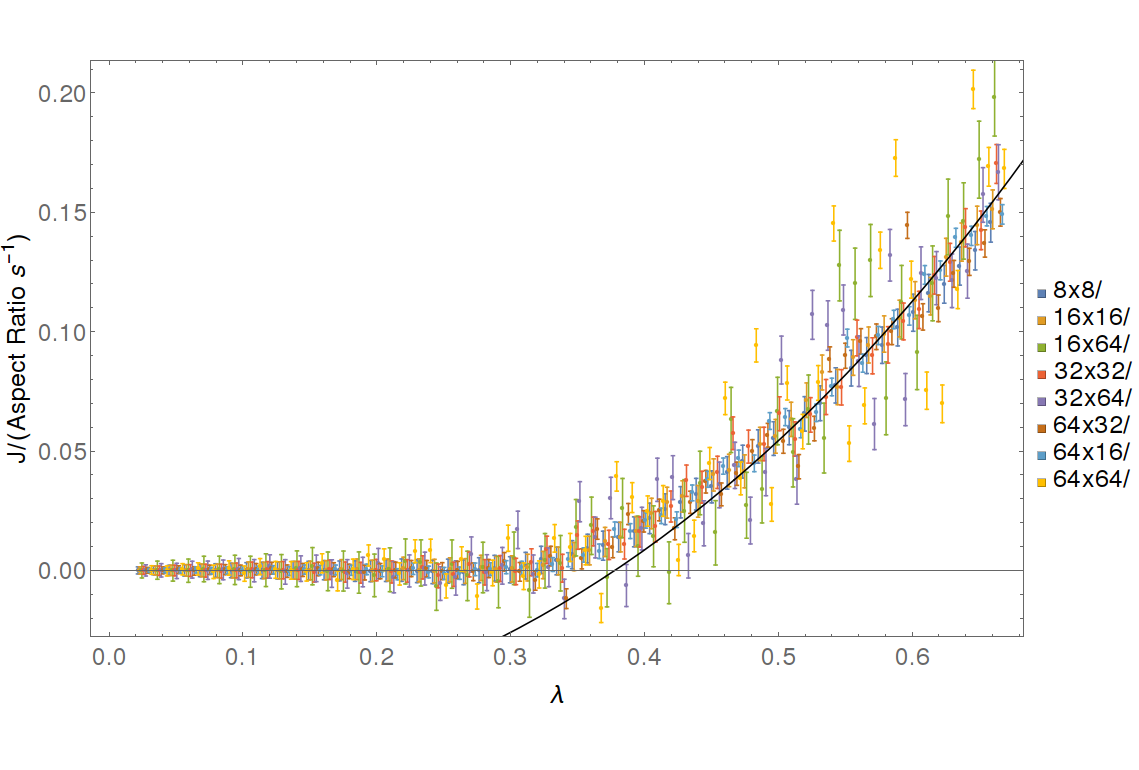
\includegraphics[width=0.95\textheight, angle=270]{numerics/images/2d/correctionFlowSizeComparison}
\end{center}
\end{figure}

Firstly, note that our supposition about the aspect ratio does appear to be true; the
data points for which the aspect ratio is $1$ line up quite nicely, and the situations
where it is $\frac{1}{2}$ or $2$ yield currents which are halved or doubled accordingly.
Notice also that the MFT prediction, whilst overestimating the actual $\lambda$ for 
which the transition occurs, is actually much better reproduced here than in $1$D, as here the
currents do indeed decrease to zero much more clearly, in line with the idea that there should be a 
hard transition. It is also worth noting that the spread of the data, generally indicative
of both convergence quality as well as the actual current fluctuation, is very large for the 
larger system sizes. Thus, we can conclude that it is probably pointless trying to measure with
system sizes of $32\times 32$ or higher, as we just cannot achieve the calculational stability
required to say anything of consequence. On the other hand, whilst the system of size $8 \times 8$
gives nicely grouped data, it is also conceptually probably too small to be useful
to us (after all, in $1$D we can perform TRM calculations with length $8$). Thus, in our
next batch of calculations we decided to use systems of size $16 \times 16$.

\subsection{Varying $\lambda$ with Constant Boundary Conditions} \label{sec:2dLambdaScans}
We intended to perform a systematic battery of calculations in $2$D just as we have done in $1$D.
However, due to the bigger issues with equilibration and overall computational time which occur in $2$D we found that performing decent calculations was much more difficult than we anticipated; thus, due to time constraints, we only managed to perform one high-quality calculation.
This is a scan through values of $\lambda$ with fixed boundary conditions, similar to our work
in Sec. \ref{sec:lambdaScans}. Here we used $L \times W = 16 \times 16$, allowed $16000000$ KMC
steps for equilibration time, and then did $4096$ measurement cycles of alternating $16000$-step
and $320000$-step analysis and relaxation runs, just like in Sec.\ref{sec:aspectRatio}. We repeated these calculations
with the same parameters with $L \times W = 32 \times 32$.
Our results for the overall system density are displayed in Fig.\ref{fig:2dSysDens}, and
our measurements of current and its variance are shown in Fig.\ref{fig:2dSysCurr}.
\begin{figure} \caption[The variation of the overall density in a $2$D SPM system with 
$\lambda$.]{The variation of the overall density in a $2$D SPM system with $\lambda$, with
$3$ sets of boundary conditions as indicated. Here diamonds indicate results taken with $L\times W=16 \times 16$,
whilst crosses indicate results with $L\times W=32\times 32$.} 
\label{fig:2dSysDens}
\begin{center}
\includegraphics[width=0.9\textheight, angle=270]{numerics/images/2d/correctionsDensBoth}
\end{center}
\end{figure}
\begin{figure} \caption[The variation of the mean current and its variance in a $2$D SPM system
with $\lambda$.]{The variation of the mean current and its variance in a $2$D SPM system
with $\lambda$, with boundary conditions as indicated. Diamonds indicate results taken with $L\times W=16 \times 16$,
crosses $L\times W=32\times 32$.} 
\label{fig:2dSysCurr}
\begin{center}
\begin{tabular}{c}
\includegraphics[width=0.95\textheight, angle=270]{numerics/images/2d/corrections2dMeans}
\end{tabular}
\end{center}
\end{figure}

Let us discuss the density results first, as without those the current results don't make as
much sense. The density changes with $\lambda$ are similar to our $1$D results in the sense
that the density attempts to converge to $1$ for extremely small values of $\lambda$ regardless
of the actual boundary conditions used, and the density has an inflection or minimum in each case for some
$\lambda$ a little below $1$.

However, there are some big differences:
\begin{itemize}
 \item The density does \textbf{not} appear to be converging to some common value regardless of
 boundaries in the large-$\lambda$ regime like it did in $1$D. A possible explanation for this
 is that there is not a straightforward family of bulk maximal-flow configurations which are
 inherently more stable than their rivals like there seems to be in $1$D; instead, due to the
 larger space of possible configurations available in $2$D, it may be the case that there are many
 different ways of realising fast rapid flow, which have different densities. An easy way to test
 this would be to perform similar calculations to these, but with a greater variety of boundary
 conditions; then, one should be able to observe whether the spectrum of densities in
 the large-$\lambda$ (repulsive) limit is continuous or discrete.
 \item For our low-density choice of boundary conditions $(\rho_0, \rho_L) = (0.3, 0.1)$,
 it would appear that the mean overall system density splits into two separate branches for the 
 $L\times W=16\times 16$ system,
 forming a curve reminiscent of the hysteresis curves exhibited by
 ferromagnets~\cite{chikazumi1997}. However, this does not seem to happen in the larger $L\times W=32\times 32$
 system. Thus, we may be probing a scenario in which the small system size allows multiple different stable
 dynamical modes to form, whilst the larger system does not support this.
\end{itemize}
So far as the current is concerned, we see broadly the same behaviour as in our (linear) plot
in Fig~\ref{fig:aspectRatios}; the current has roughly power-law dependence on $\lambda$ for
large $\lambda$, partially agreeing with the MFT prediction, before dissolving into noise
below a threshold in $\lambda$. The mean current for our low density boundary choice exhibits branching just
like
the density does, suggesting that the effective diffusion coefficients of the competing 
configurations are different. The current variance is broadly power-law with $\lambda$,
with kinks around the transitions and again some exhibition of the ``hysteresis''-like branching in the
$L\times W=16\times 16$ case.

Another way to look at this branching is to consider the fact that researchers have observed 
``stripes'' in the KLS model~\cite{Zia2010}. In that particular context the model contains asymmetric
bulk dynamics, and stripes of low and high density spontaneously form and spiral around the 
system, transmitting current as they do so. It could be the case that our $16 \times 16$ system
tries to generate such stripes, but is too small to support more than one stripe; thus, instead
different stripes are realised in different simulations. Of course, as this system is ergodic, we
should in the long-term limit see both stripe types manifest in any given simulation; however,
the switching time, if both stripe types are quite stable, might be so long that we would never
actually observe this happening. As we see no such effect in the larger system, this hypothesis seems likely.

\section{Conclusions}
The primary conclusions from our work with Monte-Carlo methods is as follows:
\begin{itemize}
 \item Our Monte-Carlo work with $1$D systems yields results very similar to those we 
 have already observed using our Transition-Rate Matrix method; thus, our fears that the small
 systems we investigated using TRM were too small to properly portray the properties of larger
 systems seem to have gone unrealised.
 \item These results appear to confirm our observation that a \textit{power law 
 switching} phenomenon does indeed occur in $1$D. Likewise they support our hypothesis that
 $1$D systems with large $\lambda$ self-organise to yield similar system configurations
 regarless of boundary conditions, in an effort to maximise flow (or more directly, system
 stability).
 \item Our foray in $2$D has been brief, but suggests that there is much more interesting material to study there, in particular the limiting behaviours with extreme $\lambda$
 and the hysteresis-curve effect we see in the density for low-density boundary configurations in small systems.
\end{itemize}




